% mnras_template.tex 
%
% LaTeX template for creating an MNRAS paper
%
% v3.0 released 14 May 2015
% (version numbers match those of mnras.cls)
%
% Copyright (C) Royal Astronomical Society 2015
% Authors:
% Keith T. Smith (Royal Astronomical Society)

% Change log
%
% v3.0 May 2015
%    Renamed to match the new package name
%    Version number matches mnras.cls
%    A few minor tweaks to wording
% v1.0 September 2013
%    Beta testing only - never publicly released
%    First version: a simple (ish) template for creating an MNRAS paper

%%%%%%%%%%%%%%%%%%%%%%%%%%%%%%%%%%%%%%%%%%%%%%%%%%
% Basic setup. Most papers should leave these options alone.
\documentclass[fleqn,usenatbib]{mnras}

% MNRAS is set in Times font. If you don't have this installed (most LaTeX
% installations will be fine) or prefer the old Computer Modern fonts, comment
% out the following line
%\usepackage{newtxtext,newtxmath}
% Depending on your LaTeX fonts installation, you might get better results with one of these:
\usepackage{mathptmx}
%\usepackage{txfonts}

% Use vector fonts, so it zooms properly in on-screen viewing software
% Don't change these lines unless you know what you are doing
\usepackage[T1]{fontenc}

% Allow "Thomas van Noord" and "Simon de Laguarde" and alike to be sorted by "N" and "L" etc. in the bibliography.
% Write the name in the bibliography as "\VAN{Noord}{Van}{van} Noord, Thomas"
\DeclareRobustCommand{\VAN}[3]{#2}
\let\VANthebibliography\thebibliography
\def\thebibliography{\DeclareRobustCommand{\VAN}[3]{##3}\VANthebibliography}


%%%%% AUTHORS - PLACE YOUR OWN PACKAGES HERE %%%%%

% Only include extra packages if you really need them. Common packages are:
\usepackage{graphicx}	% Including figure files
\usepackage{amsmath}	% Advanced maths commands
\usepackage{amssymb}	% Extra maths symbols


%%%%%%%%%%%%%%%%%%%%%%%%%%%%%%%%%%%%%%%%%%%%%%%%%%

%%%%% AUTHORS - PLACE YOUR OWN COMMANDS HERE %%%%%

% Please keep new commands to a minimum, and use \newcommand not \def to avoid
% overwriting existing commands. Example:
%\newcommand{\pcm}{\,cm$^{-2}$}	% per cm-squared

%%%%%%%%%%%%%%%%%%%%%%%%%%%%%%%%%%%%%%%%%%%%%%%%%%

%%%%%%%%%%%%%%%%%%% TITLE PAGE %%%%%%%%%%%%%%%%%%%

% Title of the paper, and the short title which is used in the headers.
% Keep the title short and informative.
\title[S-PLUS: Emission line objects]{S-PLUS: Emission line objects in the southern photometric local Universe survey}

% The list of authors, and the short list which is used in the headers.
% If you need two or more lines of authors, add an extra line using \newauthor
\author[Guti\'{e}rrez-Soto et al.]{
L. A. Guti\'{e}rrez-Soto,$^{1}$\thanks{E-mail: gsoto.angel@gmail.com}
Second  Author,$^{2}$
Third Author$^{2,3}$
and Fourth Author$^{3}$
\\
% List of institutions
$^{1}$Departamento de Astronomia, IAG, Universidade de S\~{o}a Paulo, Rua do Mata\~{o}, 1226, 05509-900, S\~{o}a Paulo, Brazil\\
$^{2}$Department, Institution, Street Address, City Postal Code, Country\\
$^{3}$Another Department, Different Institution, Street Address, City Postal Code, Country
}

% These dates will be filled out by the publisher
\date{Accepted XXX. Received YYY; in original form ZZZ}

% Enter the current year, for the copyright statements etc.
\pubyear{2021}

% Don't change these lines
\begin{document}
\label{firstpage}
\pagerange{\pageref{firstpage}--\pageref{lastpage}}
\maketitle

% Abstract of the paper
\begin{abstract}
The emission line objects are very important objects in astronomy because 
\end{abstract}

% Select between one and six entries from the list of approved keywords.
% Don't make up new ones.
\begin{keywords}
keyword1 -- keyword2 -- keyword3
\end{keywords}

%%%%%%%%%%%%%%%%%%%%%%%%%%%%%%%%%%%%%%%%%%%%%%%%%%

%%%%%%%%%%%%%%%%% BODY OF PAPER %%%%%%%%%%%%%%%%%%

\section{Introduction}

The existence of an ionizing radiation field can lead to Balmer hydrogen emission lines. From the presence  of the H Balmer lines in the optical spectra of some sources it is well known the possible presence of ionized gas. Many important astronomical objects involve the physics of photo-ionized gases and the interpretation of the emission-line spectra. Emission line objects as the H II regions allow us to study the star formation history of the far reaches of our Galaxy and of distant galaxies. Planetary nebulae let us to see the remaining envelope of dying stars. Star-burst galaxies and QSOs are one the most luminous objects and hence the most distant that can be observed. Their spectra can reveal details about of the first generation of star and the formation of heavy elements in the young universe. On the other hand, emission lines can also infer the presence or lack the accretion discs \citep{Schwope:2000, Ratti:2012}, the properties of single or double picked line can allow us to infer geometrical characteristics \citep{Horne:1986}, the nature of  donor stars in binary system \citep{Steeghs:2002, Spaandonk:2010, Casares:2015} and the compact objects as black holes \citep{Casares:2016}. 

Emission lines are also associated with stars in very early-type and/or very late evolutionary stage which are short phase. As already mentioned are also associated with binaries that experiencing mass transfer. These group of emission line stars includes young stellar (YSOs) and Herbig-Haro (HH) objects, post-asymptotic and some asymptotic giant branch (AGB), some red giant stars (RGB), Wolf-Rayet (WR) stars, supernova remnants, classical Be stars, active late-type dwarfs, interacting binary system like symbiotic stars (SySt) and cataclysmic variables (CV). Most of these class of object are in-homogeneous and some contains many few identified members, for instance at the moment around 323 symbiotic system have been identified from which 257 belong to the Galaxy and  $\sim$66 are extra-galactic objects (Akras et al. 2019). The same occurs with PNe from witch around 3500 of them are been cataloged, this current number of PNe represents only about 15-30\% of the estimated total of Galactic PNe (Frew, 2008; Jacoby et al., 2010) showing that a small fraction of the PNe have been cataloged (Frew, 2017). Many galaxies, in addition to harbor Planetary nebulae and H II regions, show characteristic nebular in their spectra. In most of these objects, the gas is photoionized by hot stars in the nucleus, which is thus much like giant H II region, or perhaps many H II regions. The galactic nucleus with very strongest  emission lines of this type are often called blue compact galaxies, extragaltic H II regions, star forming or starburst galaxies (Osterbrock 2006).

In the past H$\lpha$ surveys with modest spatial resolutions have been used to identified extended nebular emission to study supernova remnants, galaxy groups and star forming regions (Davies, Elliott & Meaburn 1976). More recently,  







% \texttt{mnras\_sample.tex} for a more complex example, and \texttt{mnras\_guide.tex}

% \citet{Fournier1901},
% \citep[e.g.][]{vanDijk1902}.
% \citet{deLaguarde1903, delaGuarde1904}.


\section{Observations}
\label{sec:obser}

The S-PLUS survey is a multi-band photometric survey...

\begin{figure}
	% To include a figure from a file named example.*
	% Allowable file formats are eps or ps if compiling using latex
	% or pdf, png, jpg if compiling using pdflatex
	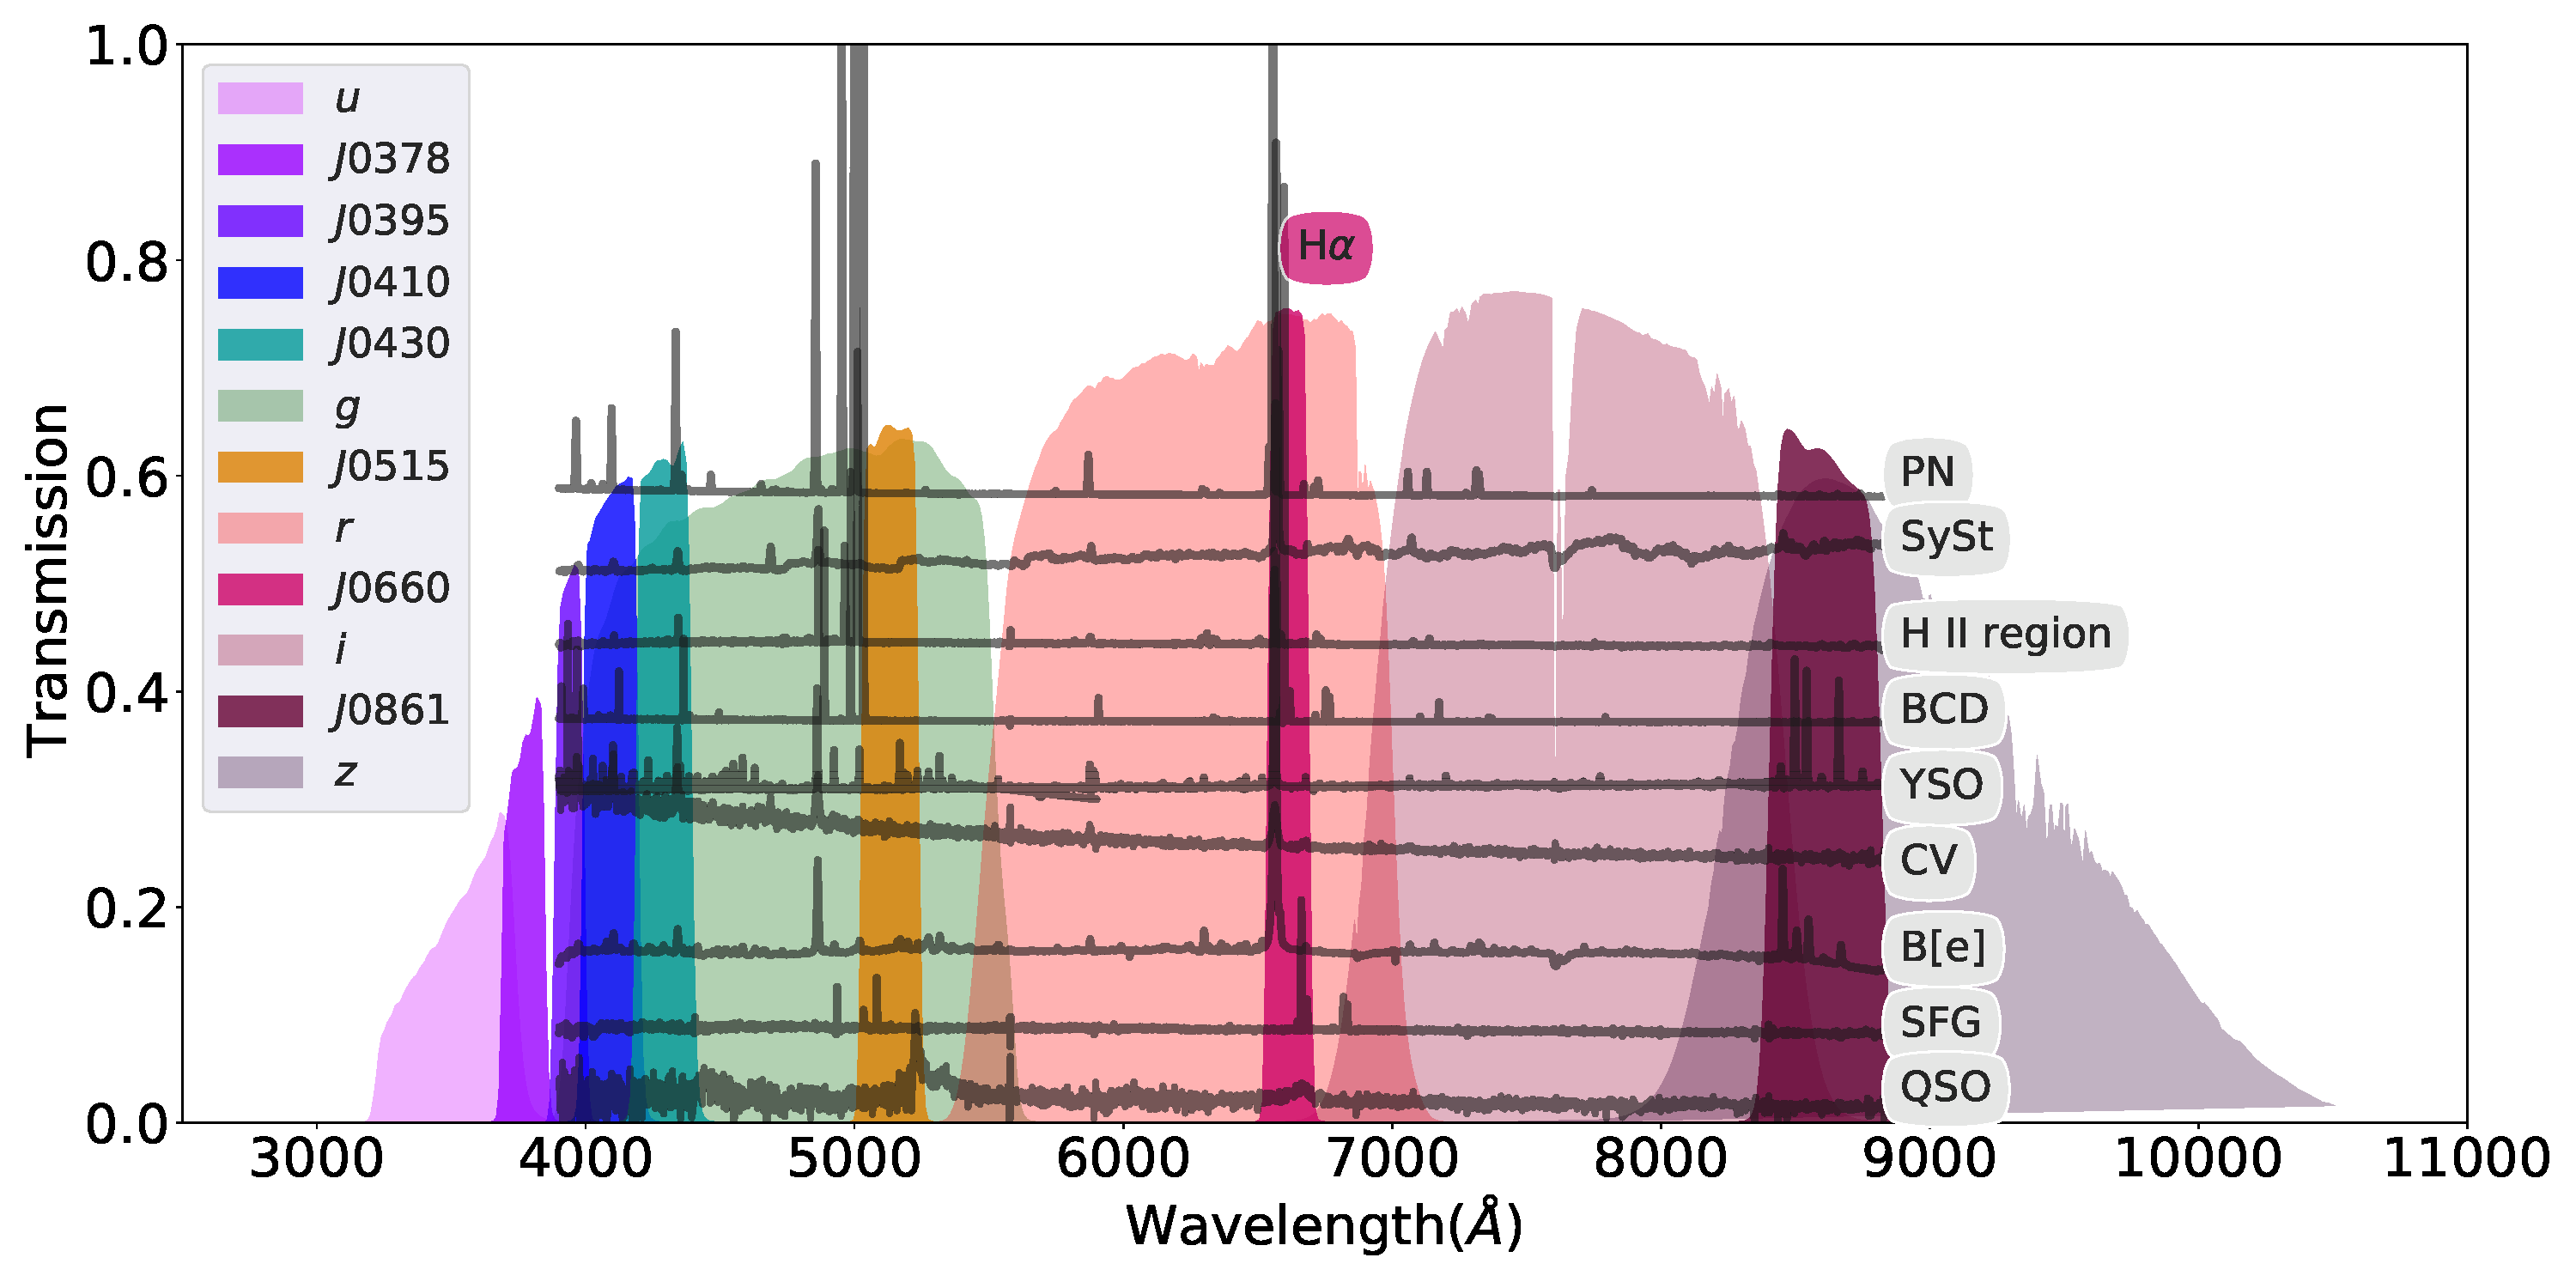
\includegraphics[width=0.9\linewidth]{Figs/splus-filter.pdf}
    \caption{Transmission curves...}
    \label{fig:curves}
\end{figure}


\section{Methodology}
\label{sec:meth}

\citet{Witham:2008} presented a catalogue of point-sources H{$\alpha$} emission objects identified in IPHAS. 

Appliyng the selection criteria to selecting H$\alpha$ emitters. We used the same procedure in Wevers et al. (2017). The objects with H$\alpha$ excess meet the condition:

 $(r - J0660)_{obs} - (r - J0660)_{fit} \geq C \times \sqrt{\sigma^2_s - \sigma^2_{phot}}$ 
 
where $\sigma_s$ is the root mean squared value of the residuals around
the fit and $\sigma_{phot}$ is the error on the observed $(r - J0660)$ colour

Firts see an aproximation of the  4$\sigma$ cut away from the ariginal fit.

\begin{figure*}
  \setlength\tabcolsep{0pt}
  \setkeys{Gin}{width=0.5\linewidth}
  \begin{tabular}{ll}
    (a) & (b) \\
    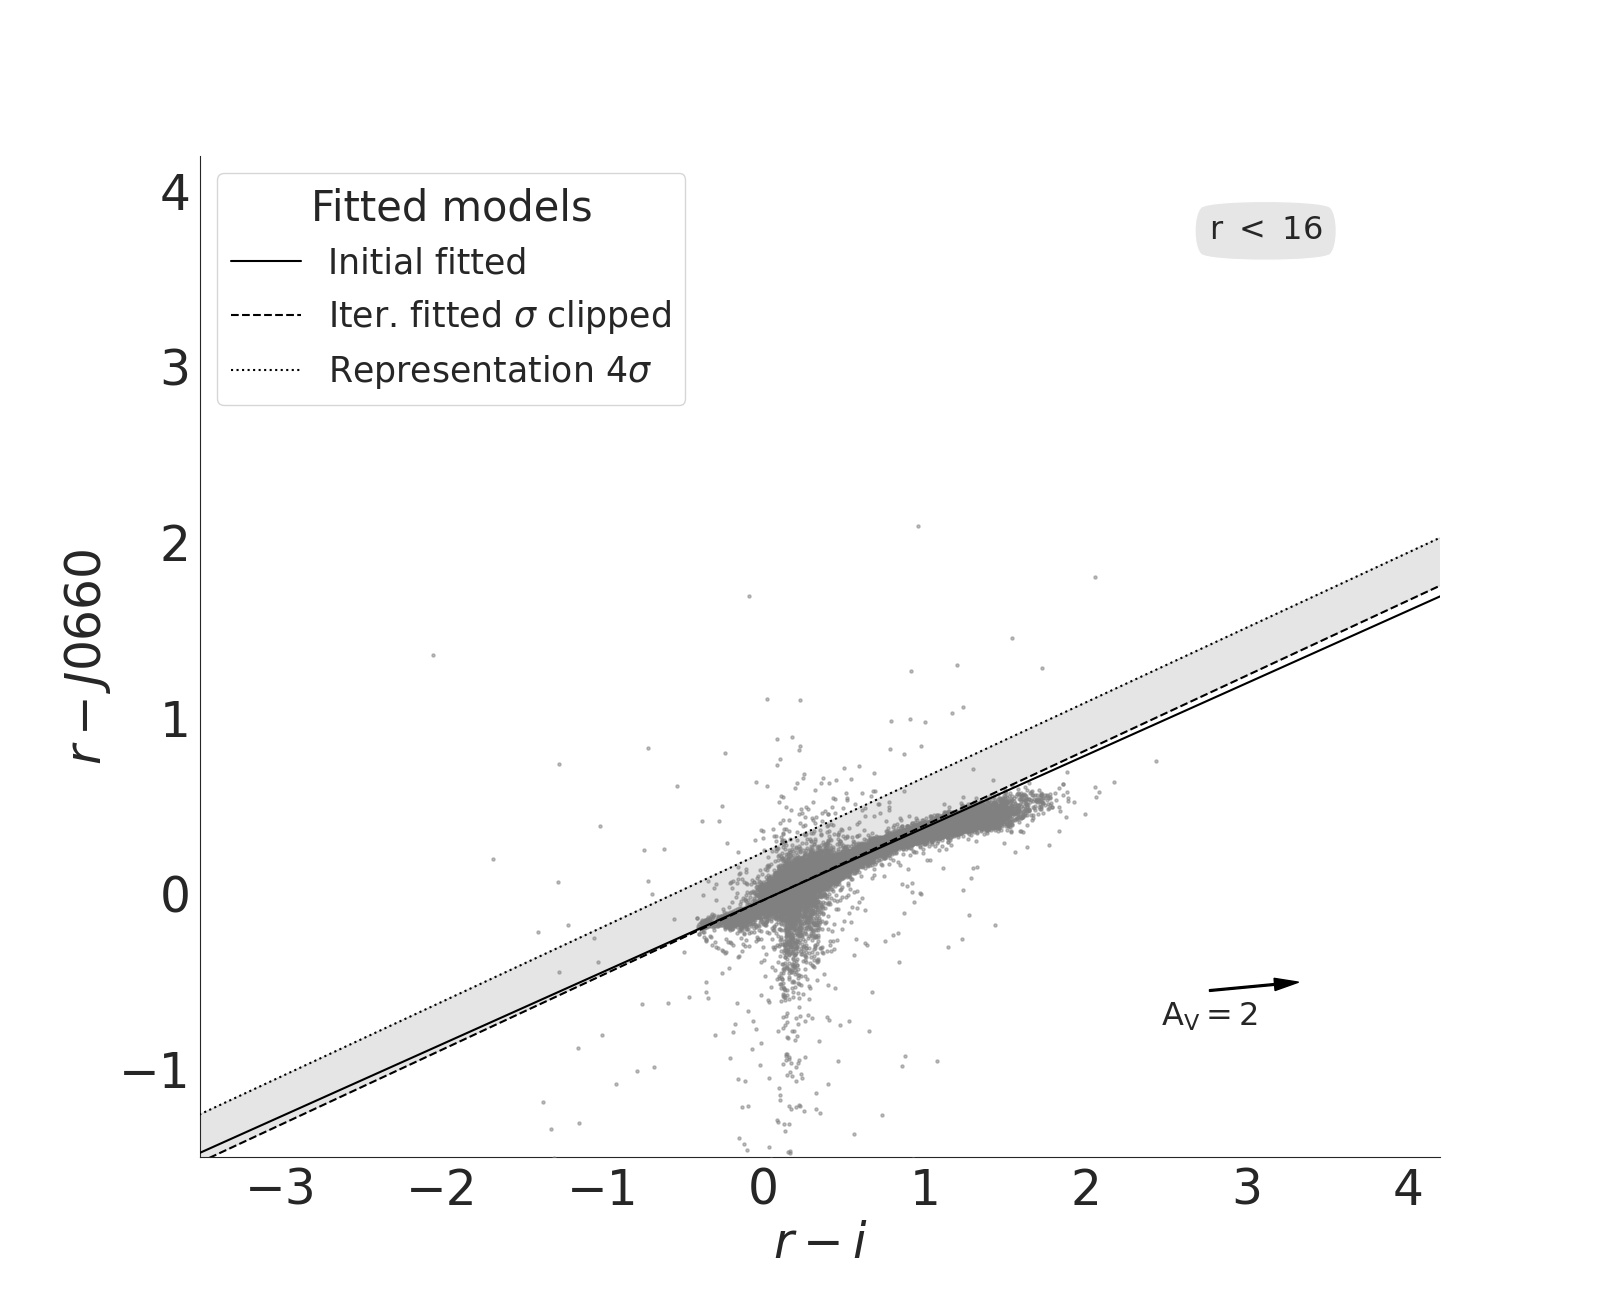
\includegraphics[trim=10 0 65 20, clip]{Figs/diagram-DR3-errorFlag0-3f-16r}
    & 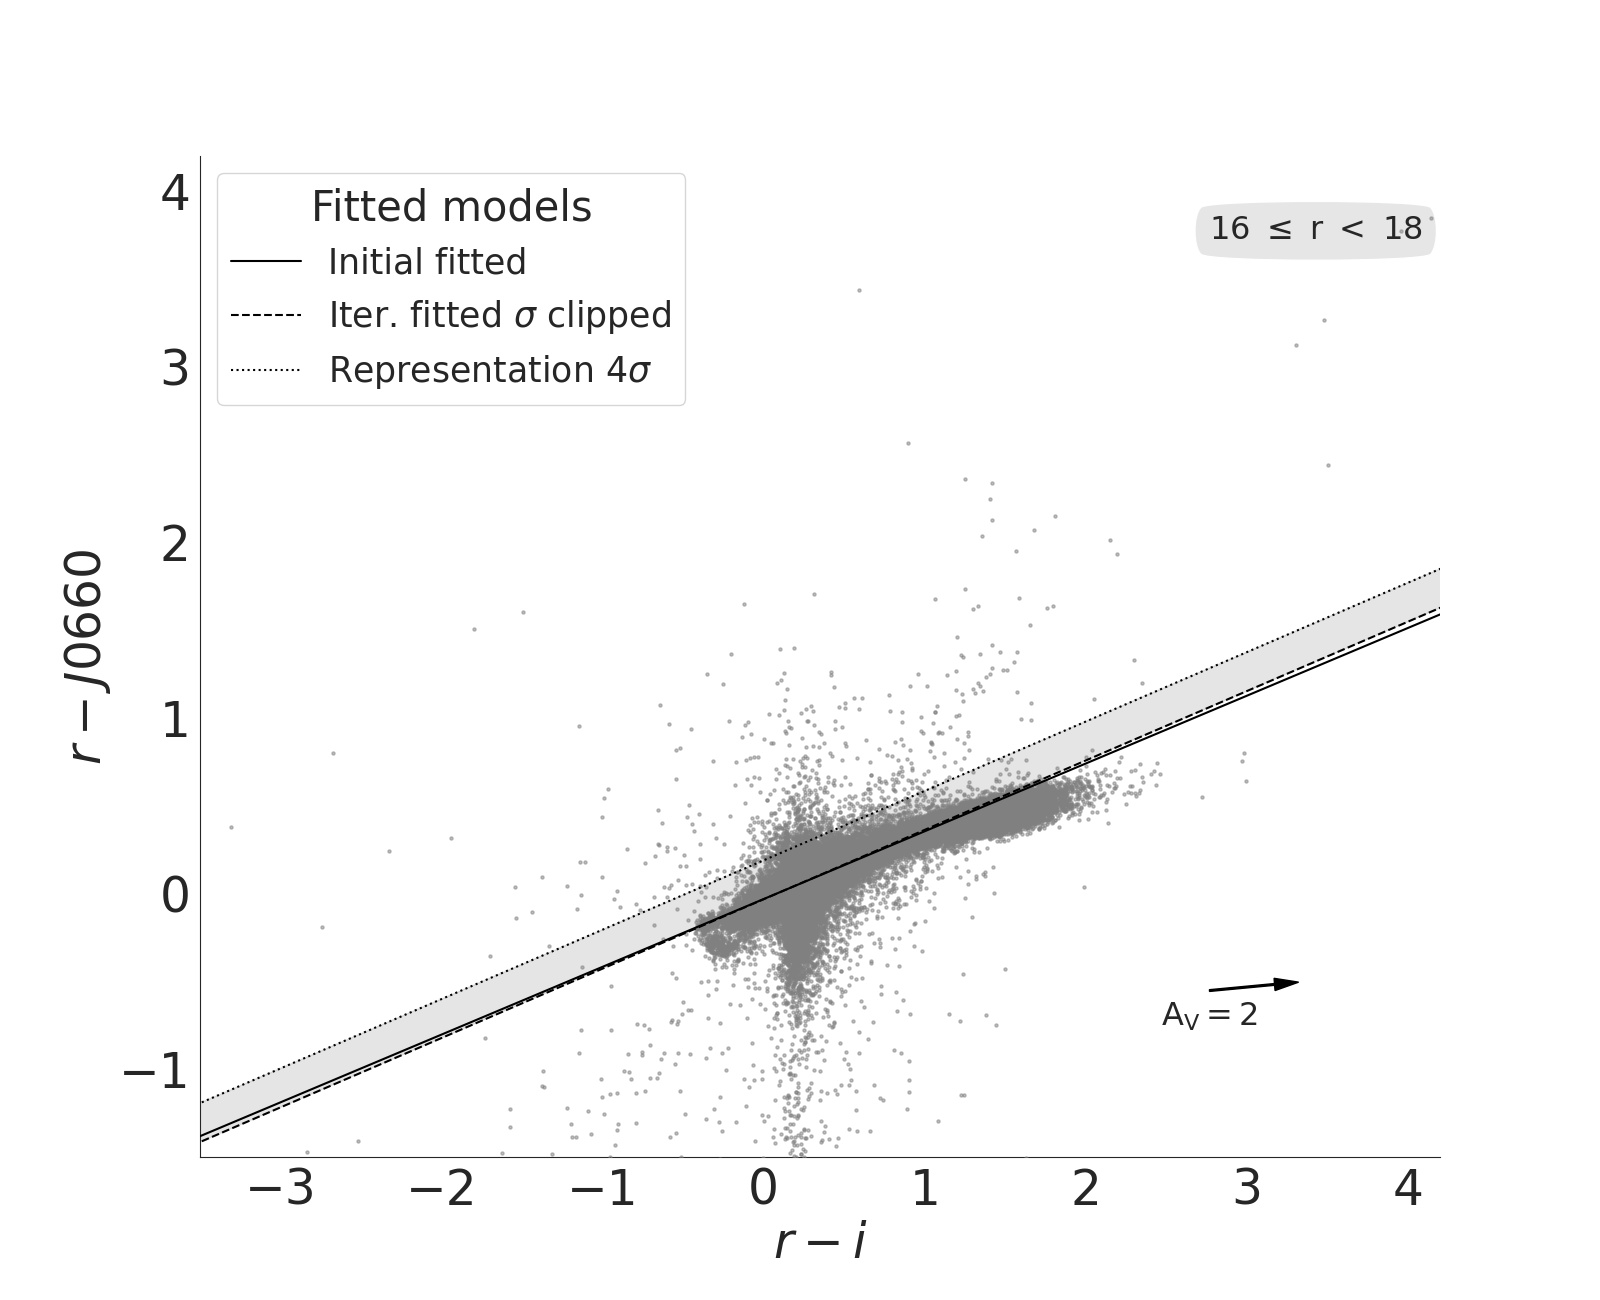
\includegraphics[trim=10 0 65 20, clip]{Figs/diagram-DR3-errorFlag0-3f-16r18}\\
    (c) & (d) \\
    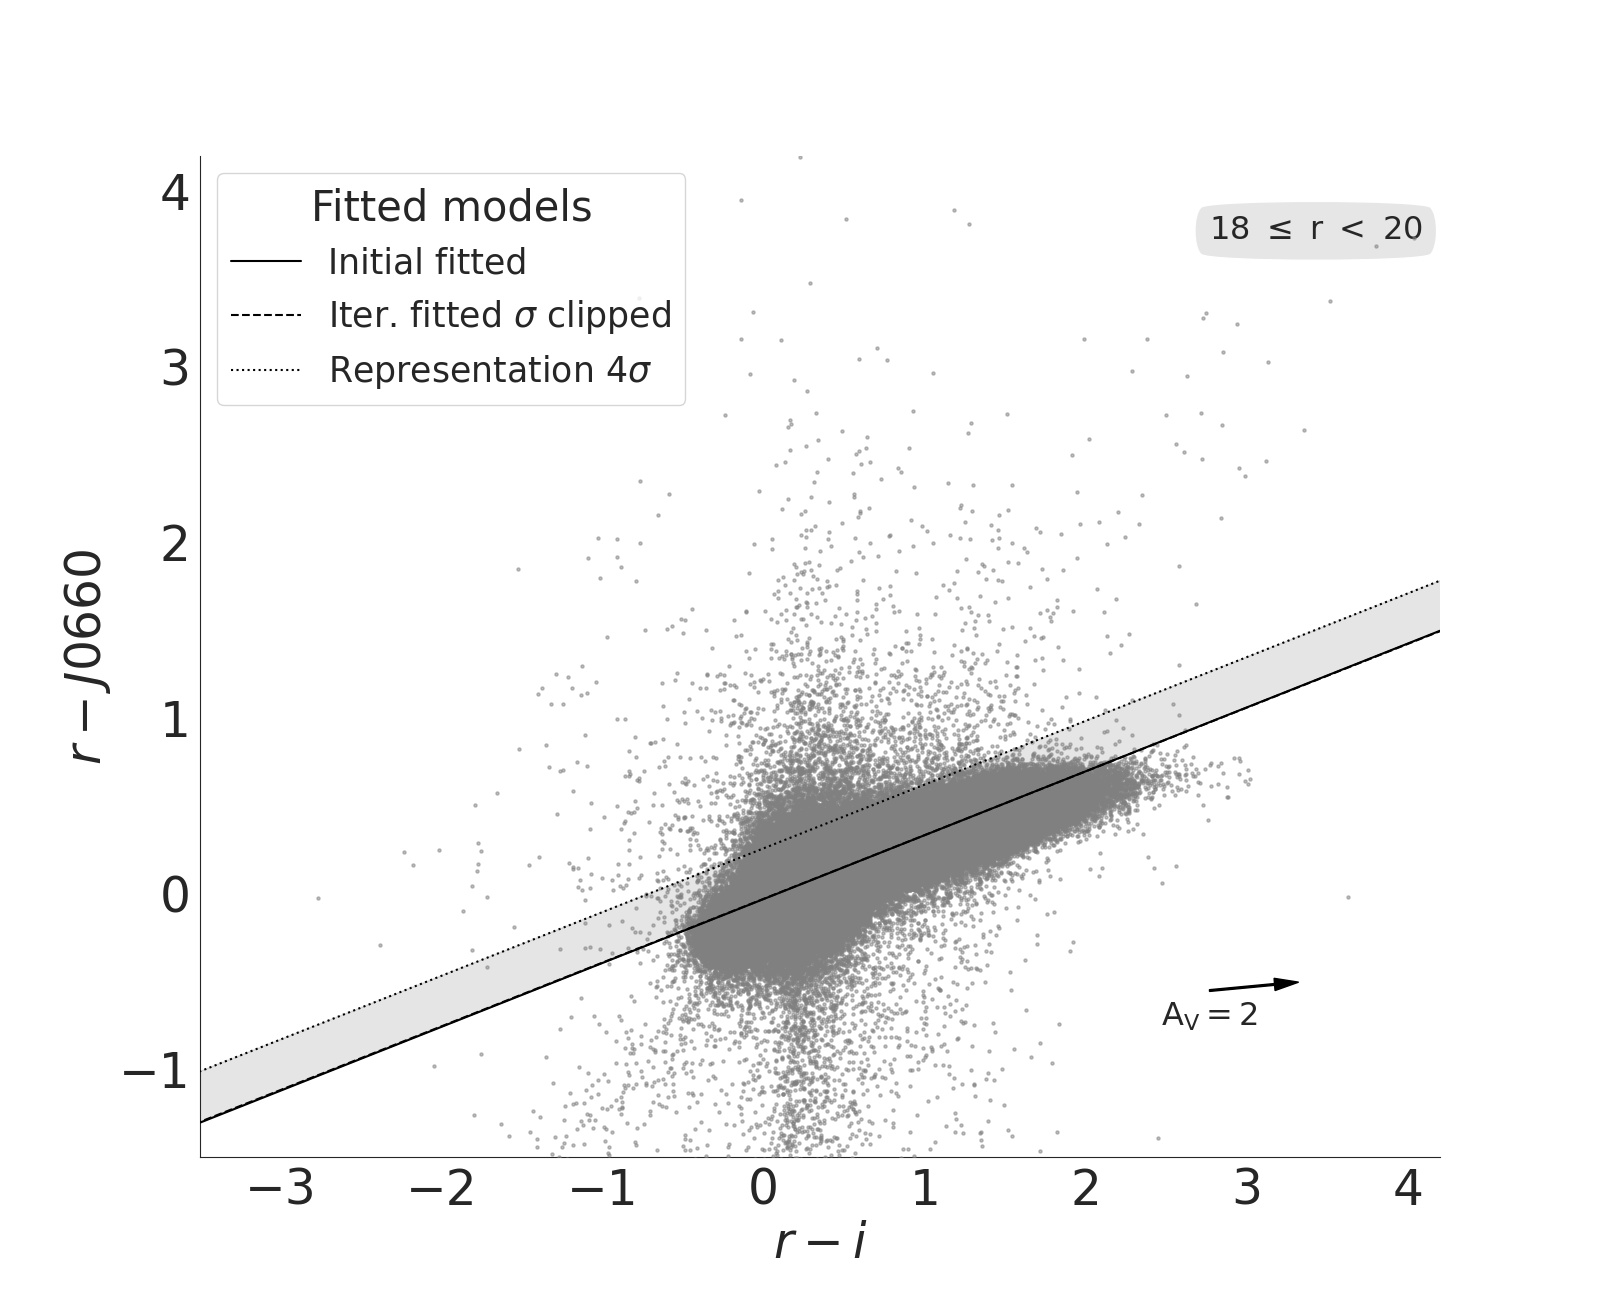
\includegraphics[trim=10 0 65 20, clip]{Figs/diagram-DR3-errorFlag0-3f-18r20}
    & 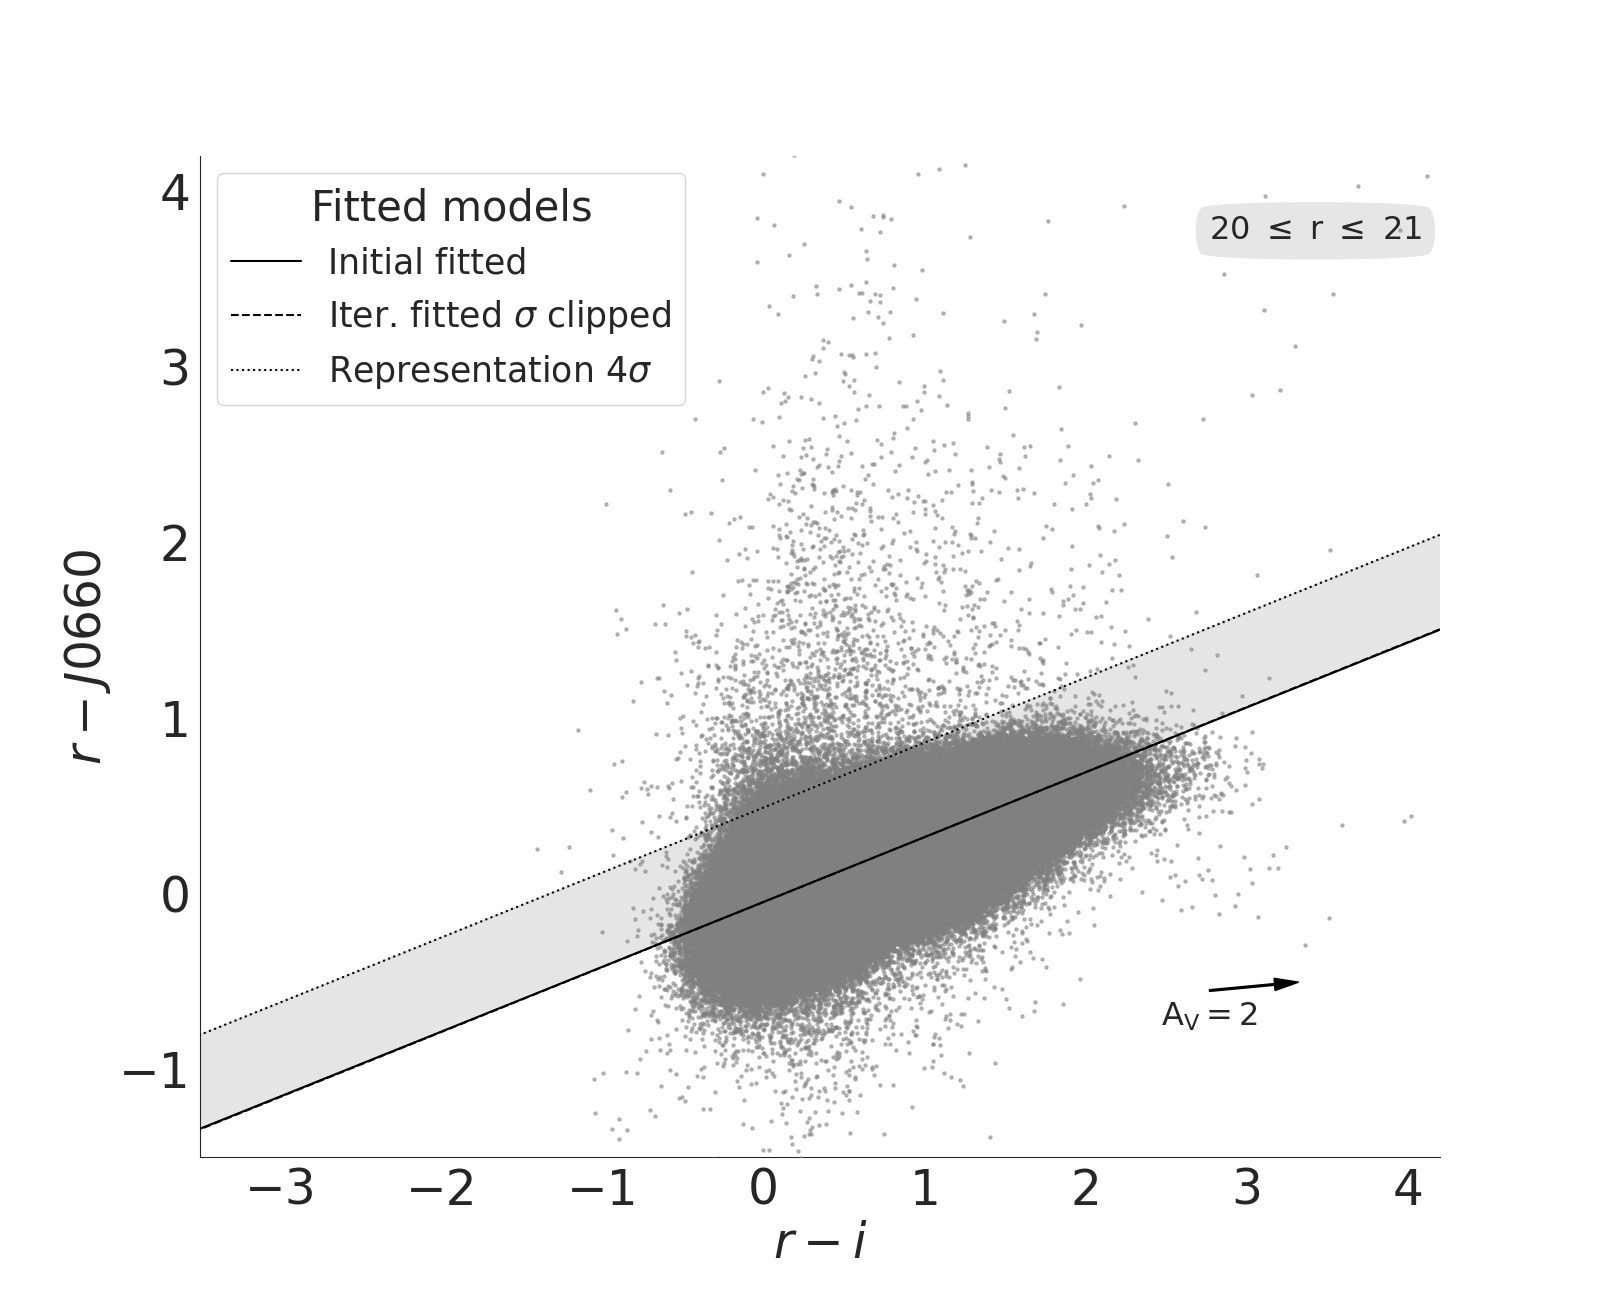
\includegraphics[trim=10 0 65 20, clip]{Figs/diagram-DR3-errorFlag0-3f-20r21}\\
  \end{tabular}
  \caption{Color-color diagrams with all objects...}
  \label{fig:color-diagram}
\end{figure*}


%It is frequently split into subsections, such as Section~\ref{sec:maths} below.

\subsection{Maths}
\label{sec:maths} % used for referring to this section from elsewhere

 %% e.g. $2\times3=6$
%% or $v=220$\,km\,s$^{-1}$, but more complicated expressions should be entered


\begin{equation}

    x=\frac{-b\pm\sqrt{b^2-4ac}}{2a}.
	\label{eq:quadratic}
\end{equation}

%Refer back to them as e.g. equation~(\ref{eq:quadratic}).

\subsection{Figures and tables}

\section{Results}
\label{sec:results}

\begin{figure*}
	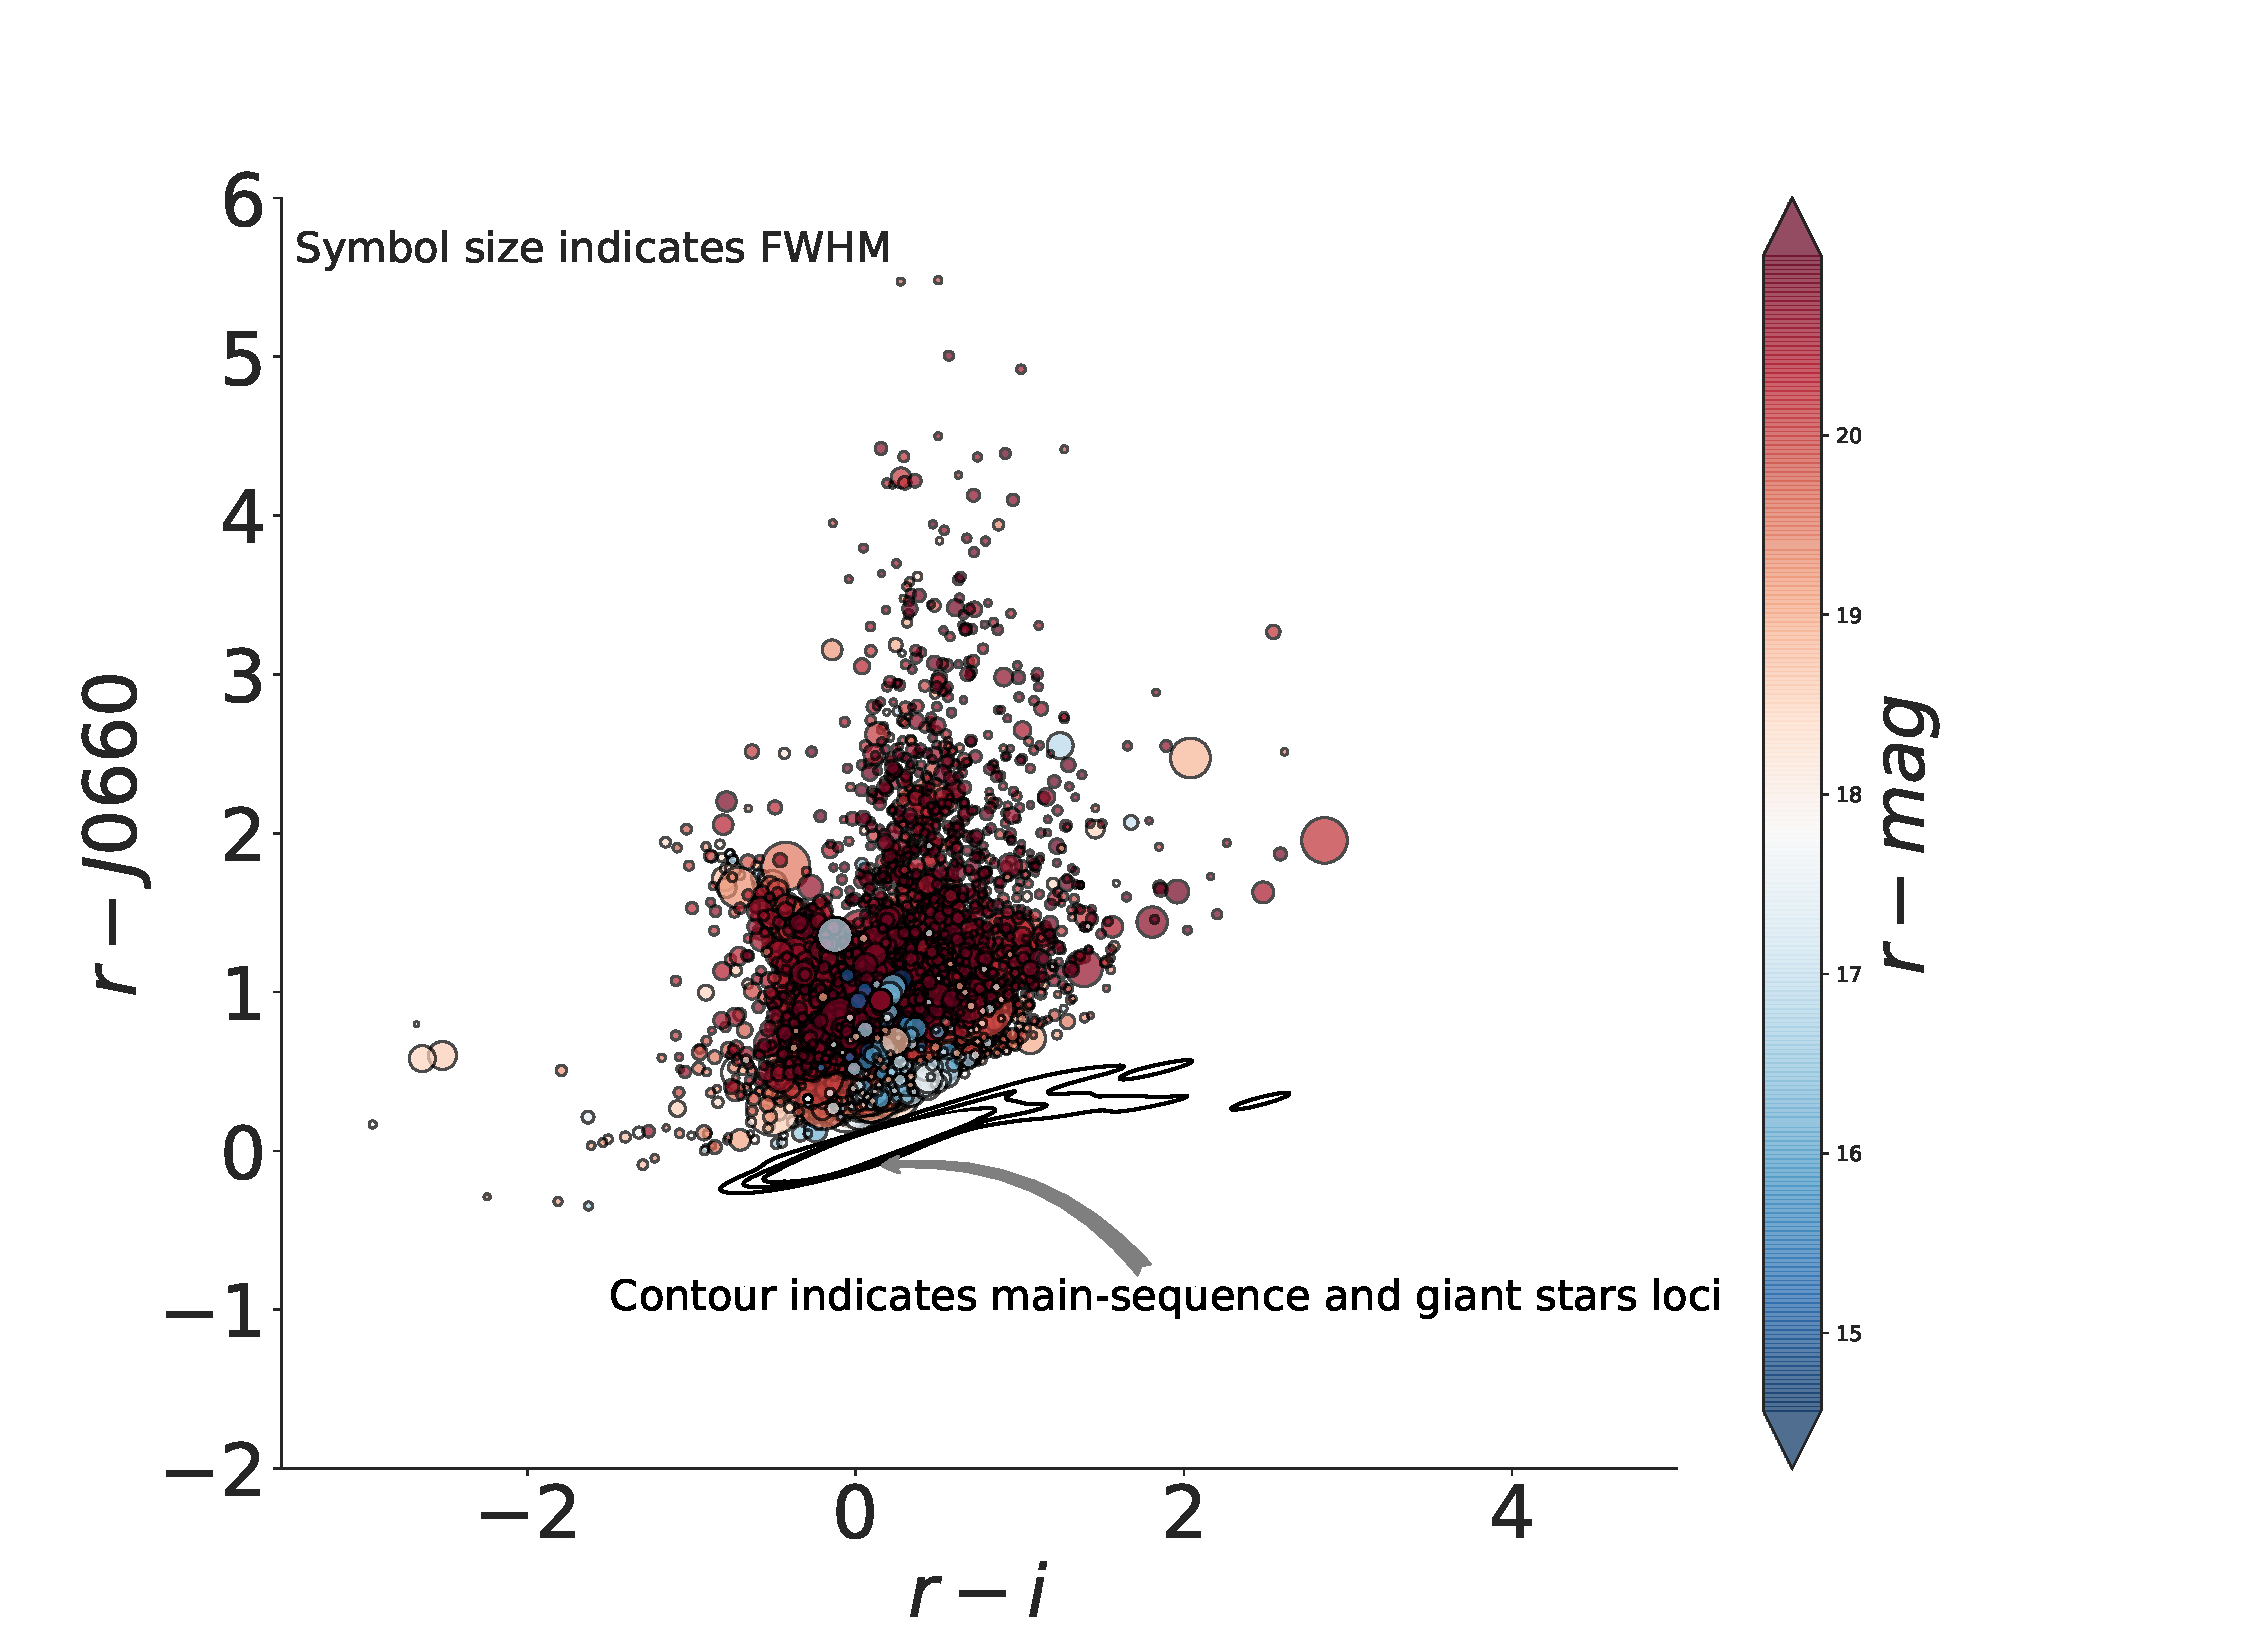
\includegraphics[width=0.9\linewidth]{Figs/final-emitters.pdf}
    \caption{Emission lines selected...}
    \label{fig:emission}
\end{figure*}

\begin{figure*}
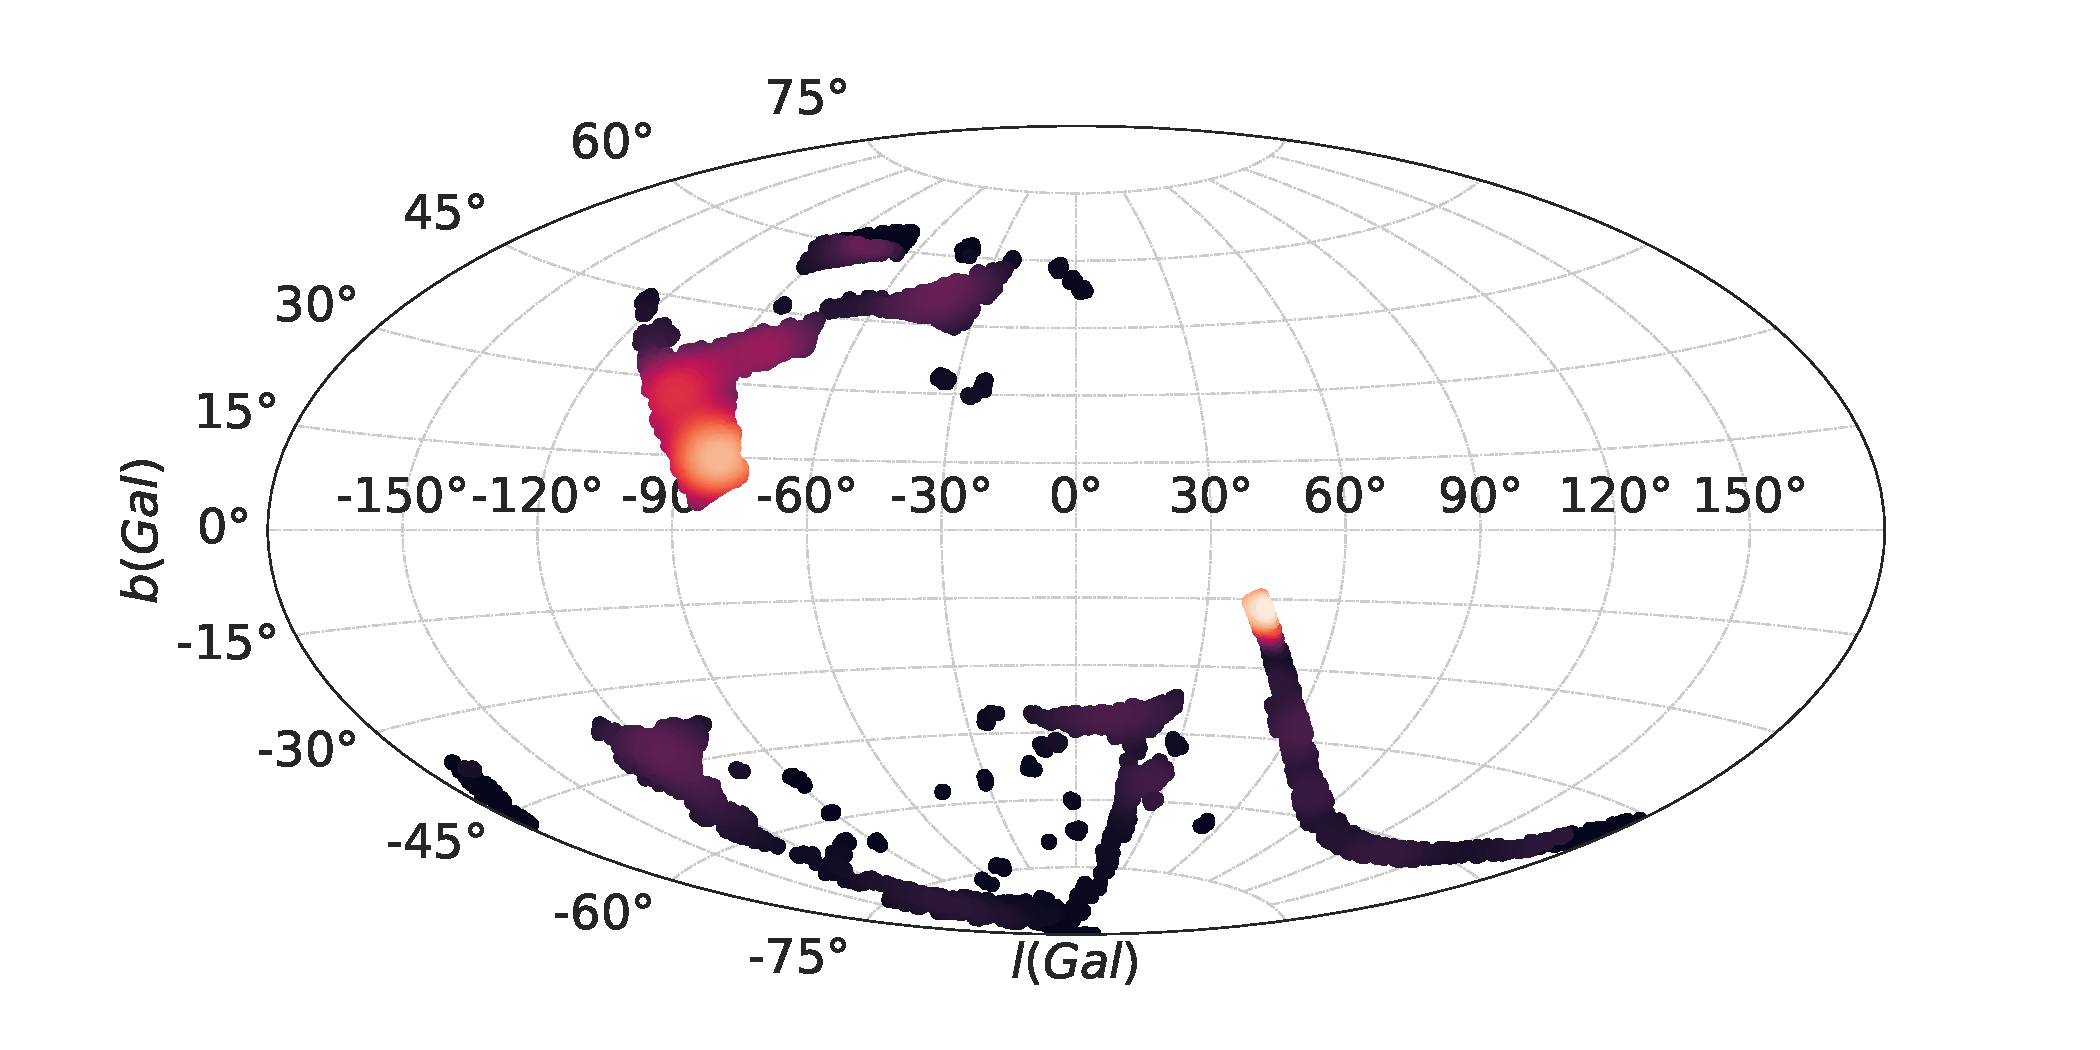
\includegraphics[width=0.9\linewidth]{Figs/halpha-emitters-galactic-aitoff.pdf}
\centering
\llap{\shortstack{%
        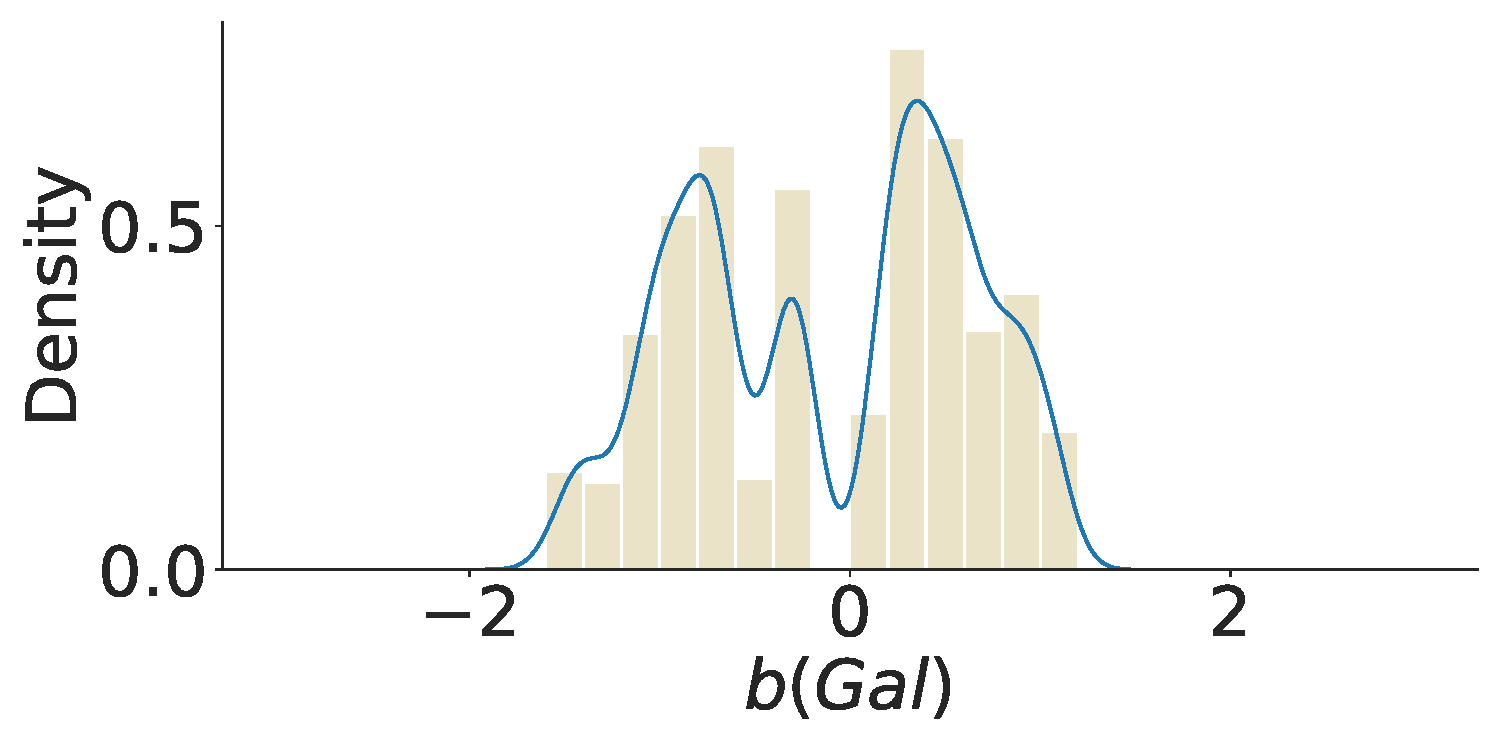
\includegraphics[width=0.25\linewidth, trim=10 10 -40 0]{Figs/distribution-bgalactic.pdf}\\
        \rule{0ex}{1.8in}%
      }
  \rule{1.0in}{0ex}}
\caption{This is my embedded figure}
\end{figure*}


\begin{figure*}
  \begin{tabular}{l l l}
  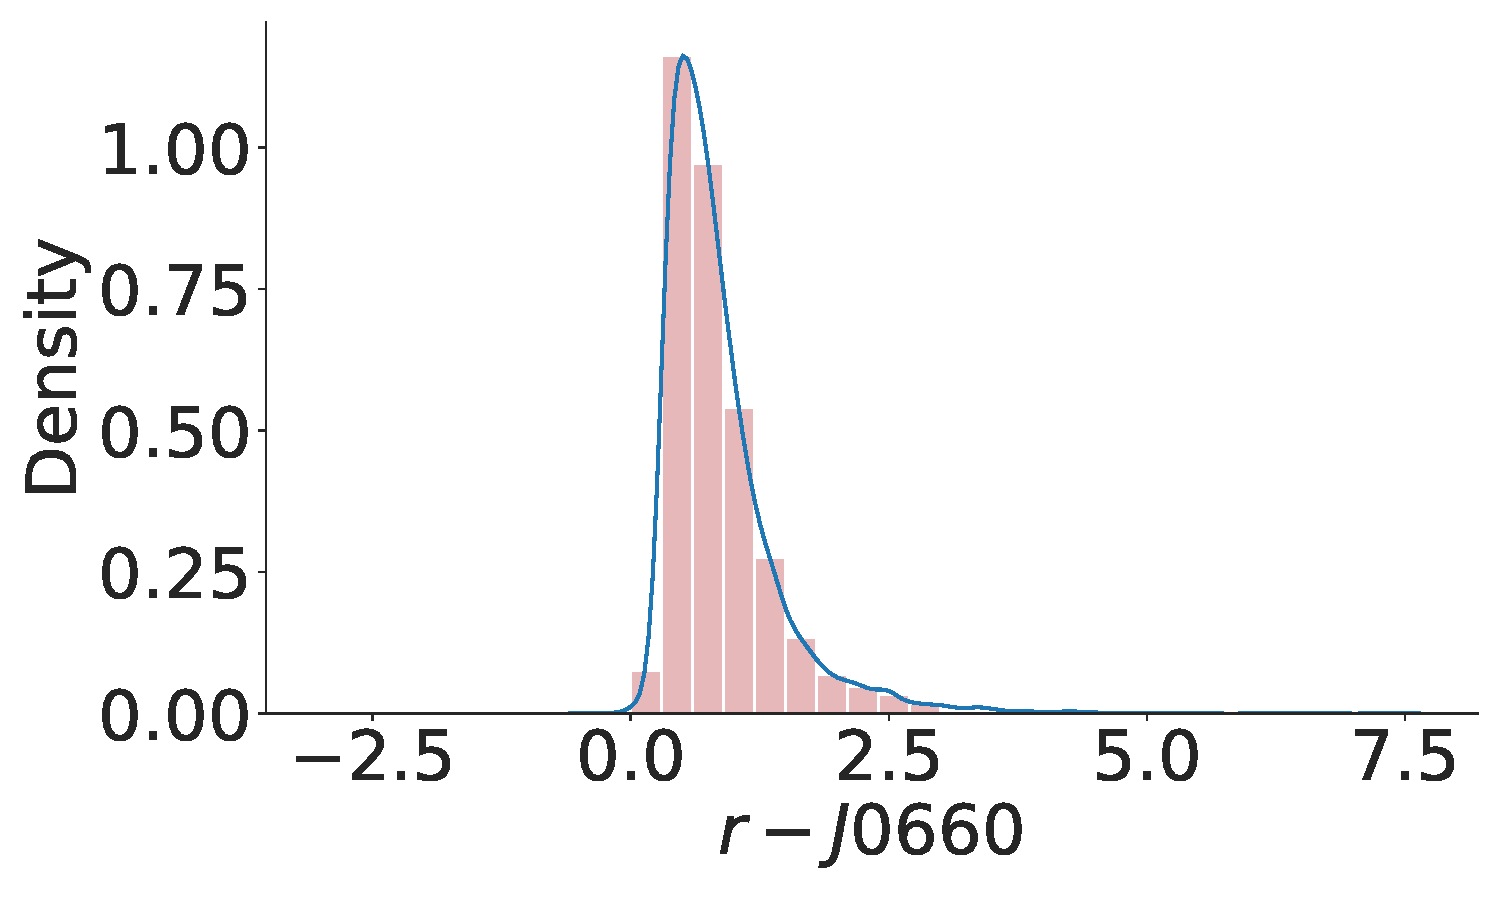
\includegraphics[width=0.7\columnwidth]{Figs/distribution-Halpha.pdf} 
    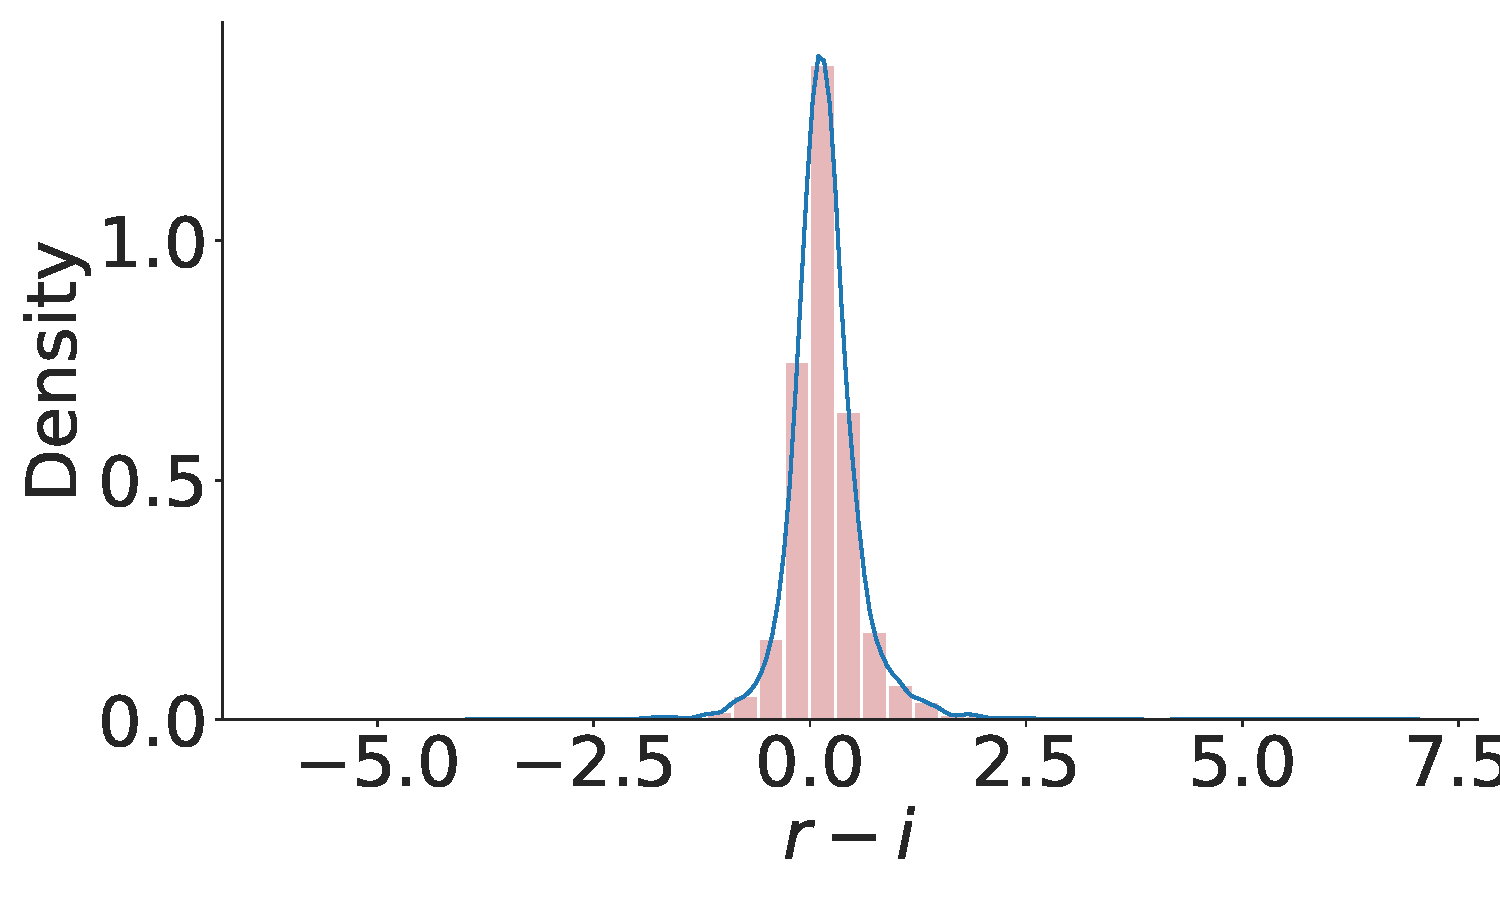
\includegraphics[width=0.7\columnwidth]{Figs/distribution-ri.pdf}
    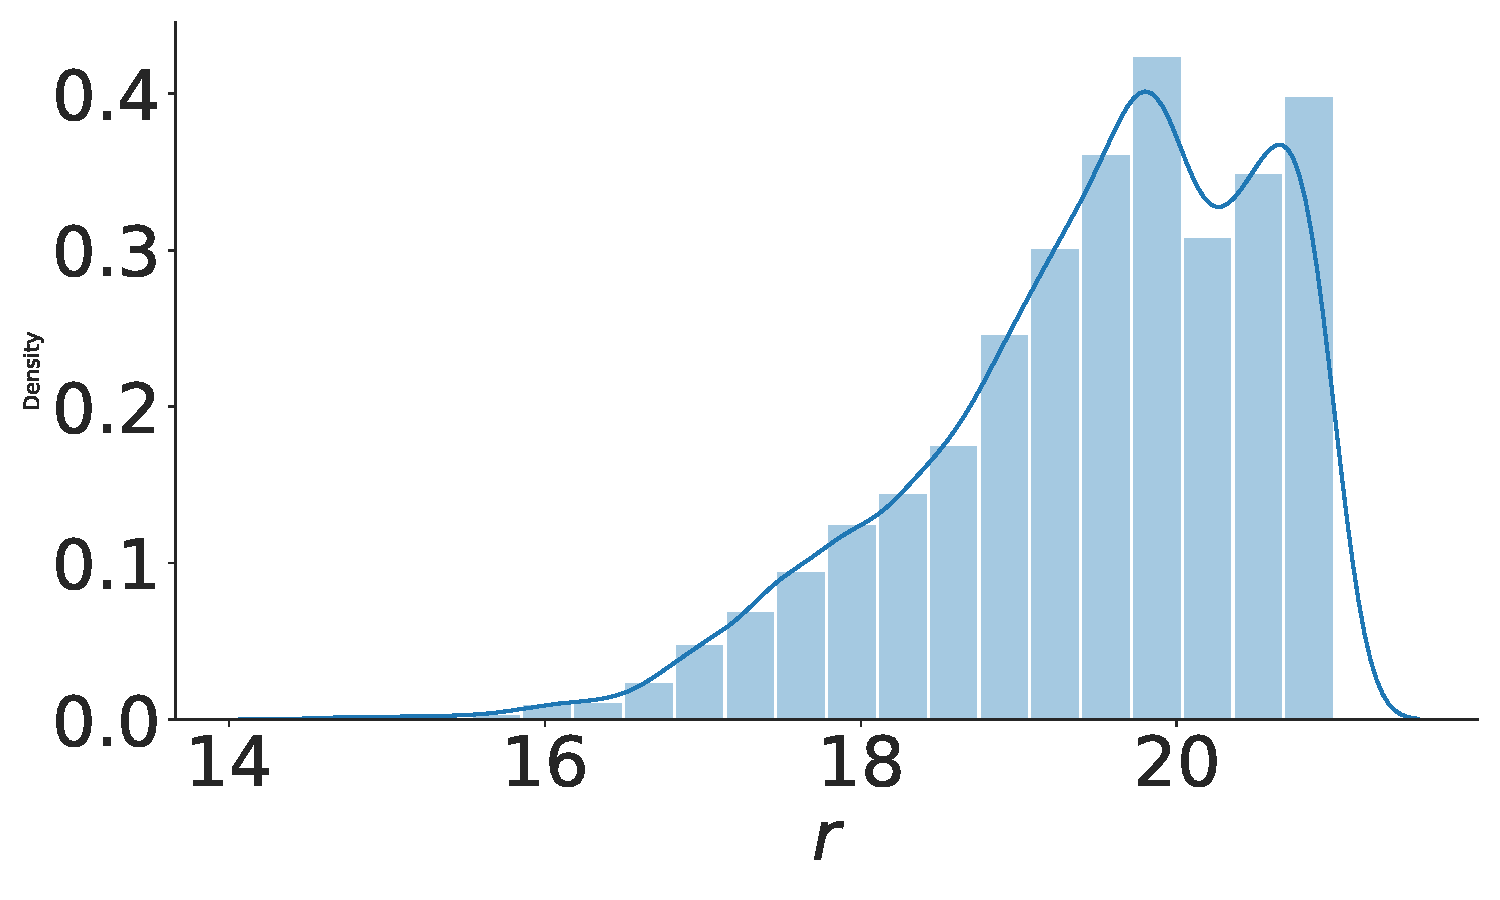
\includegraphics[width=0.7\columnwidth]{Figs/distribution_r.pdf}
  \end{tabular}
    \caption{Emission lines selected...}
    \label{fig:diagram-distri}
\end{figure*}

\begin{figure}
	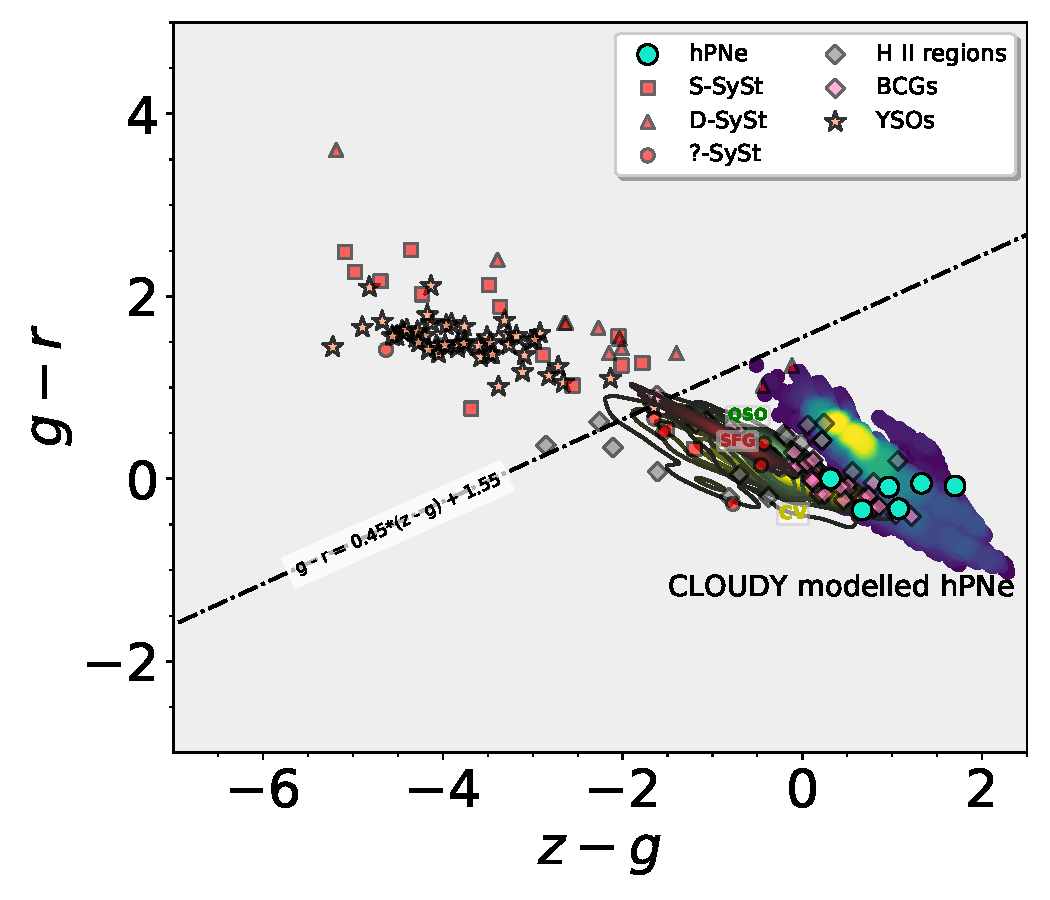
\includegraphics[width=0.9\linewidth]{Figs/Fig-SPLUS-gr-zg.pdf}
    \caption{Classifying...}
    \label{fig:cluster}
\end{figure}

\begin{figure*}
\centering
\begin{tabular}{l l}
  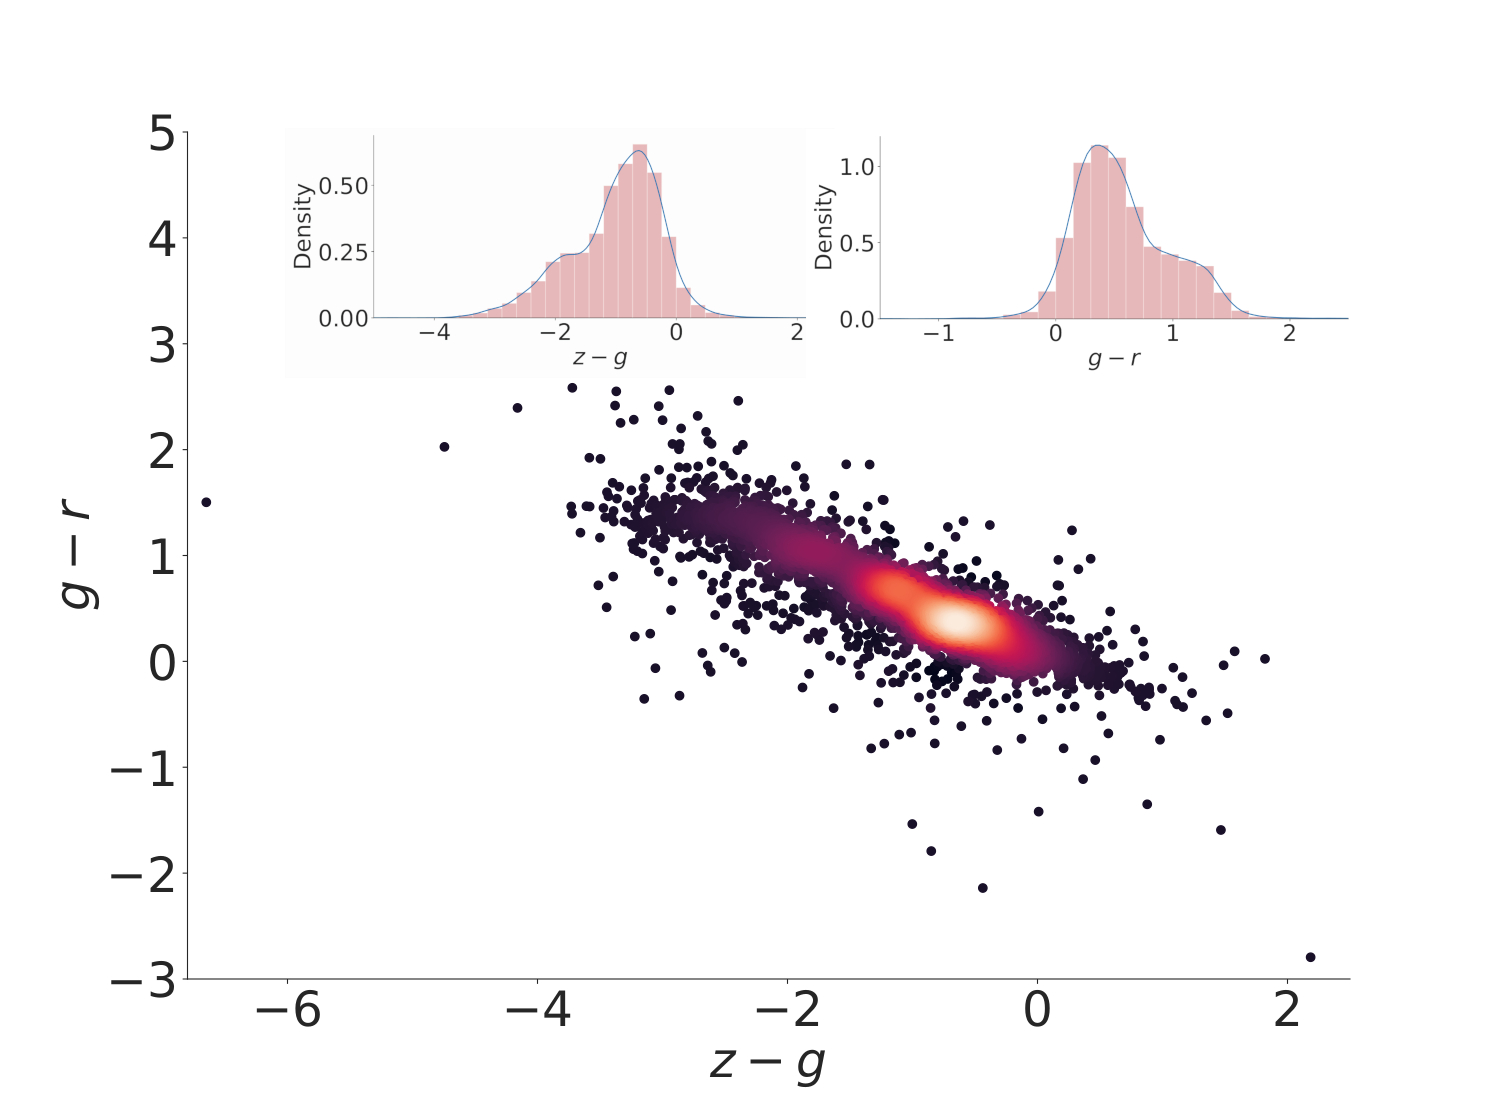
\includegraphics[width=0.6\linewidth, trim=10 10 5 8, clip]{Figs/red-blue-colorObjects-gr-edit.jpg}
   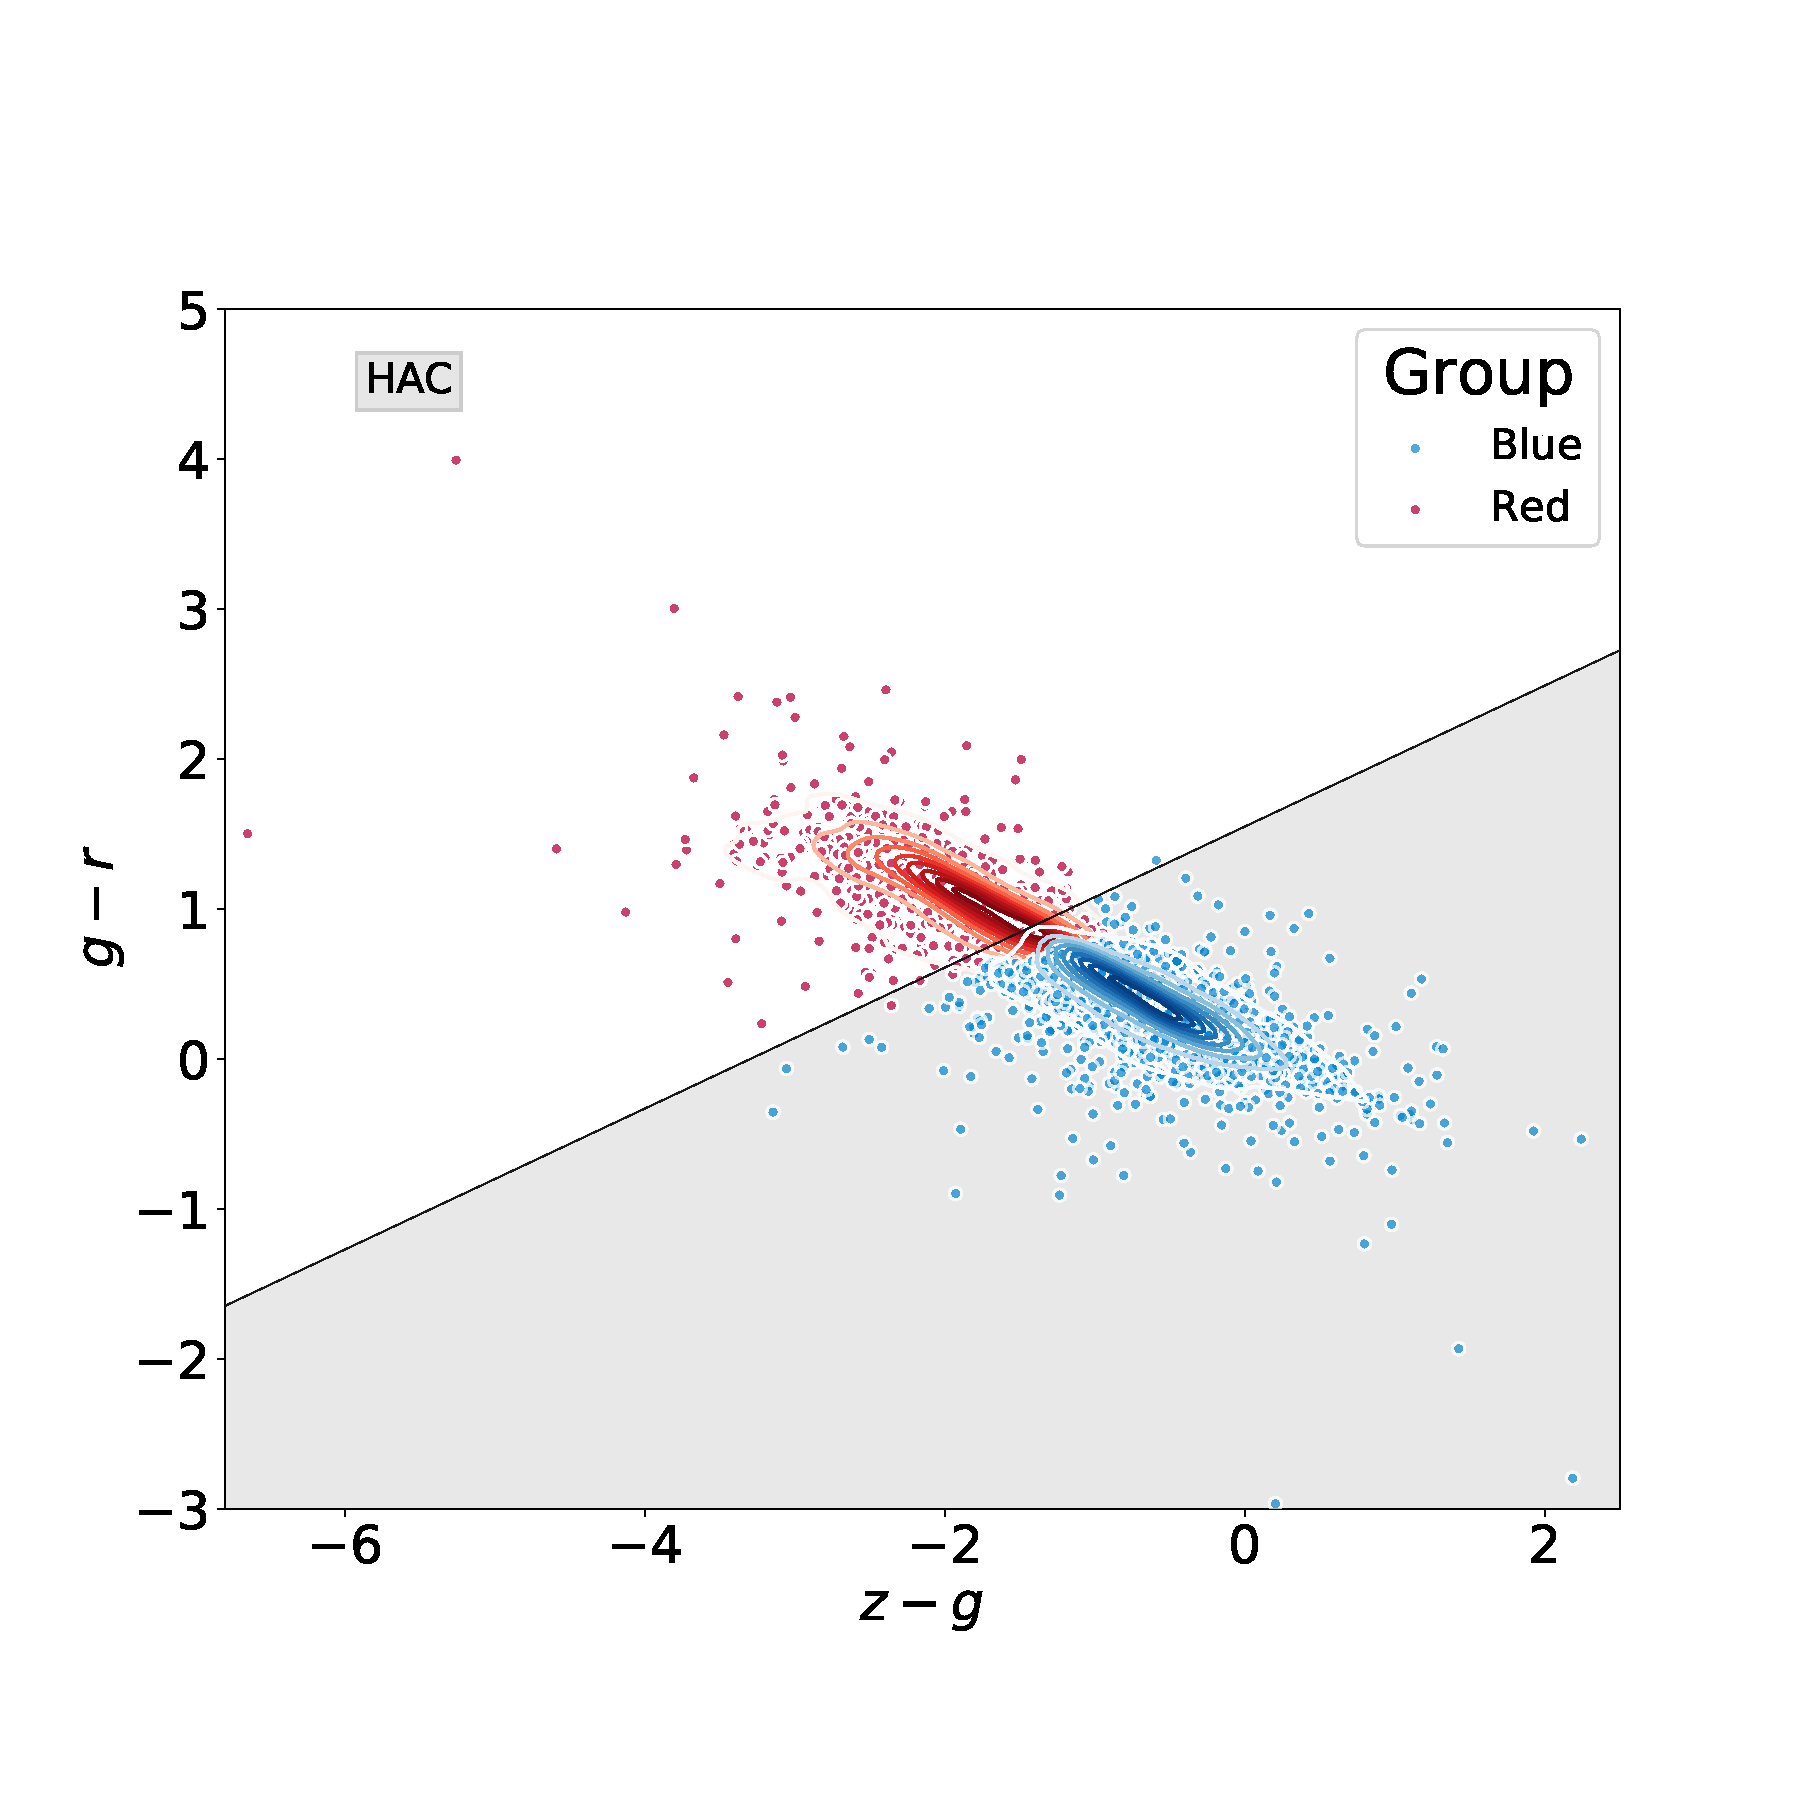
\includegraphics[width=0.5\linewidth, trim=10 10 5 8. clip]{Figs/blued-red-hierarchical.pdf}
  \end{tabular}  
  \caption{New color-color diagram to separate the blue objects from the red ones.}
\label{fig:new-color}
\end{figure*}


\begin{figure*}
  \setlength\tabcolsep{0pt}
  \setkeys{Gin}{width=0.5\linewidth}
  \begin{tabular}{ll}
    (a) & (b) \\
    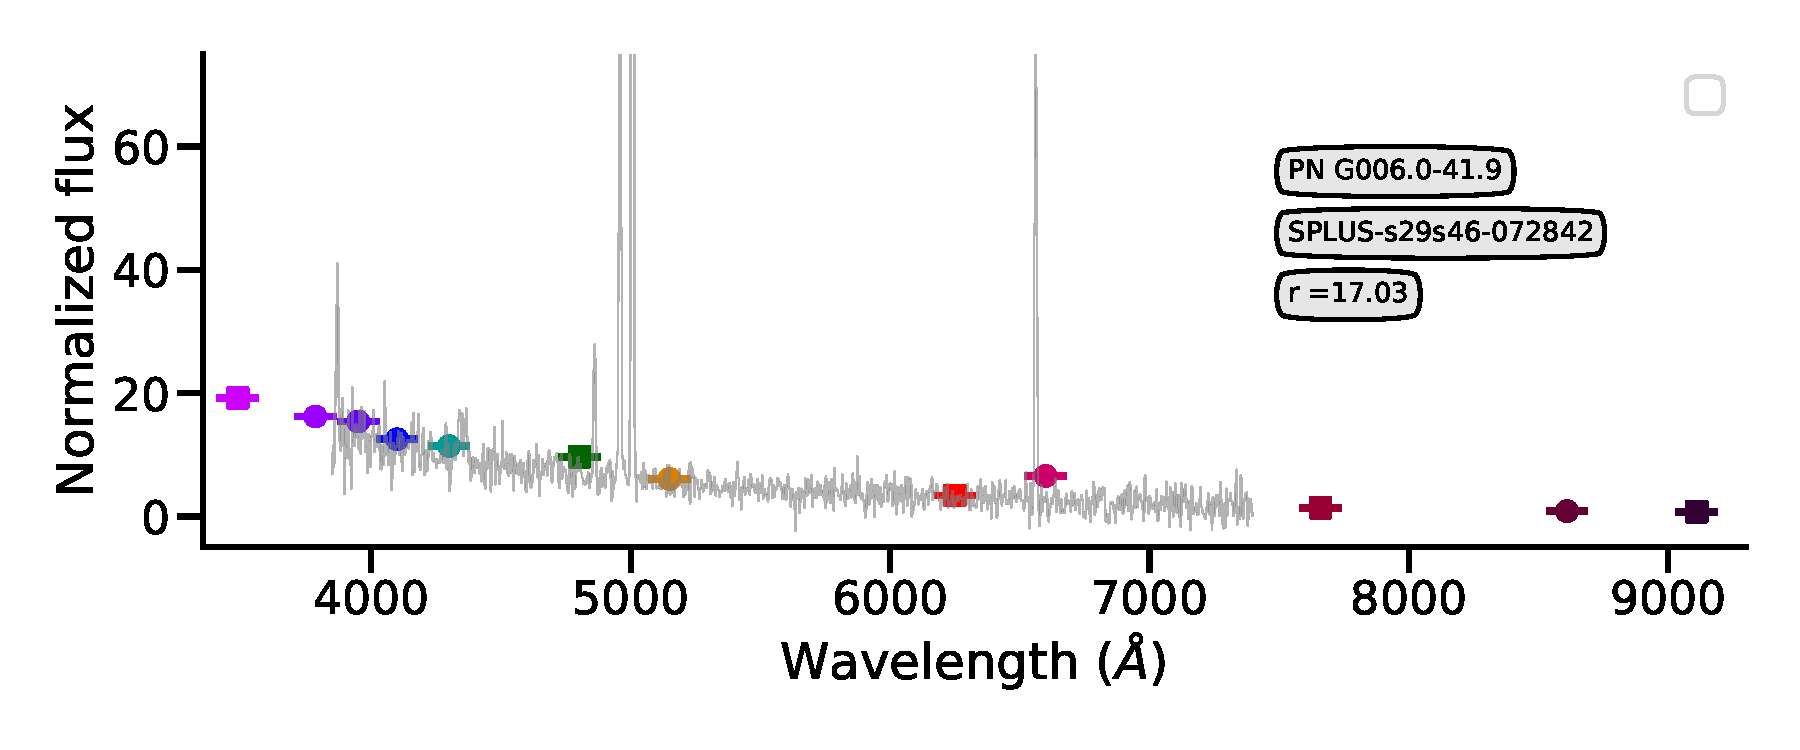
\includegraphics[trim=10 0 10 20, clip]{Figs/StenholmAcker_pn_g006_0-41_9_id176-SPLUS-s29s46-072842.pdf} & 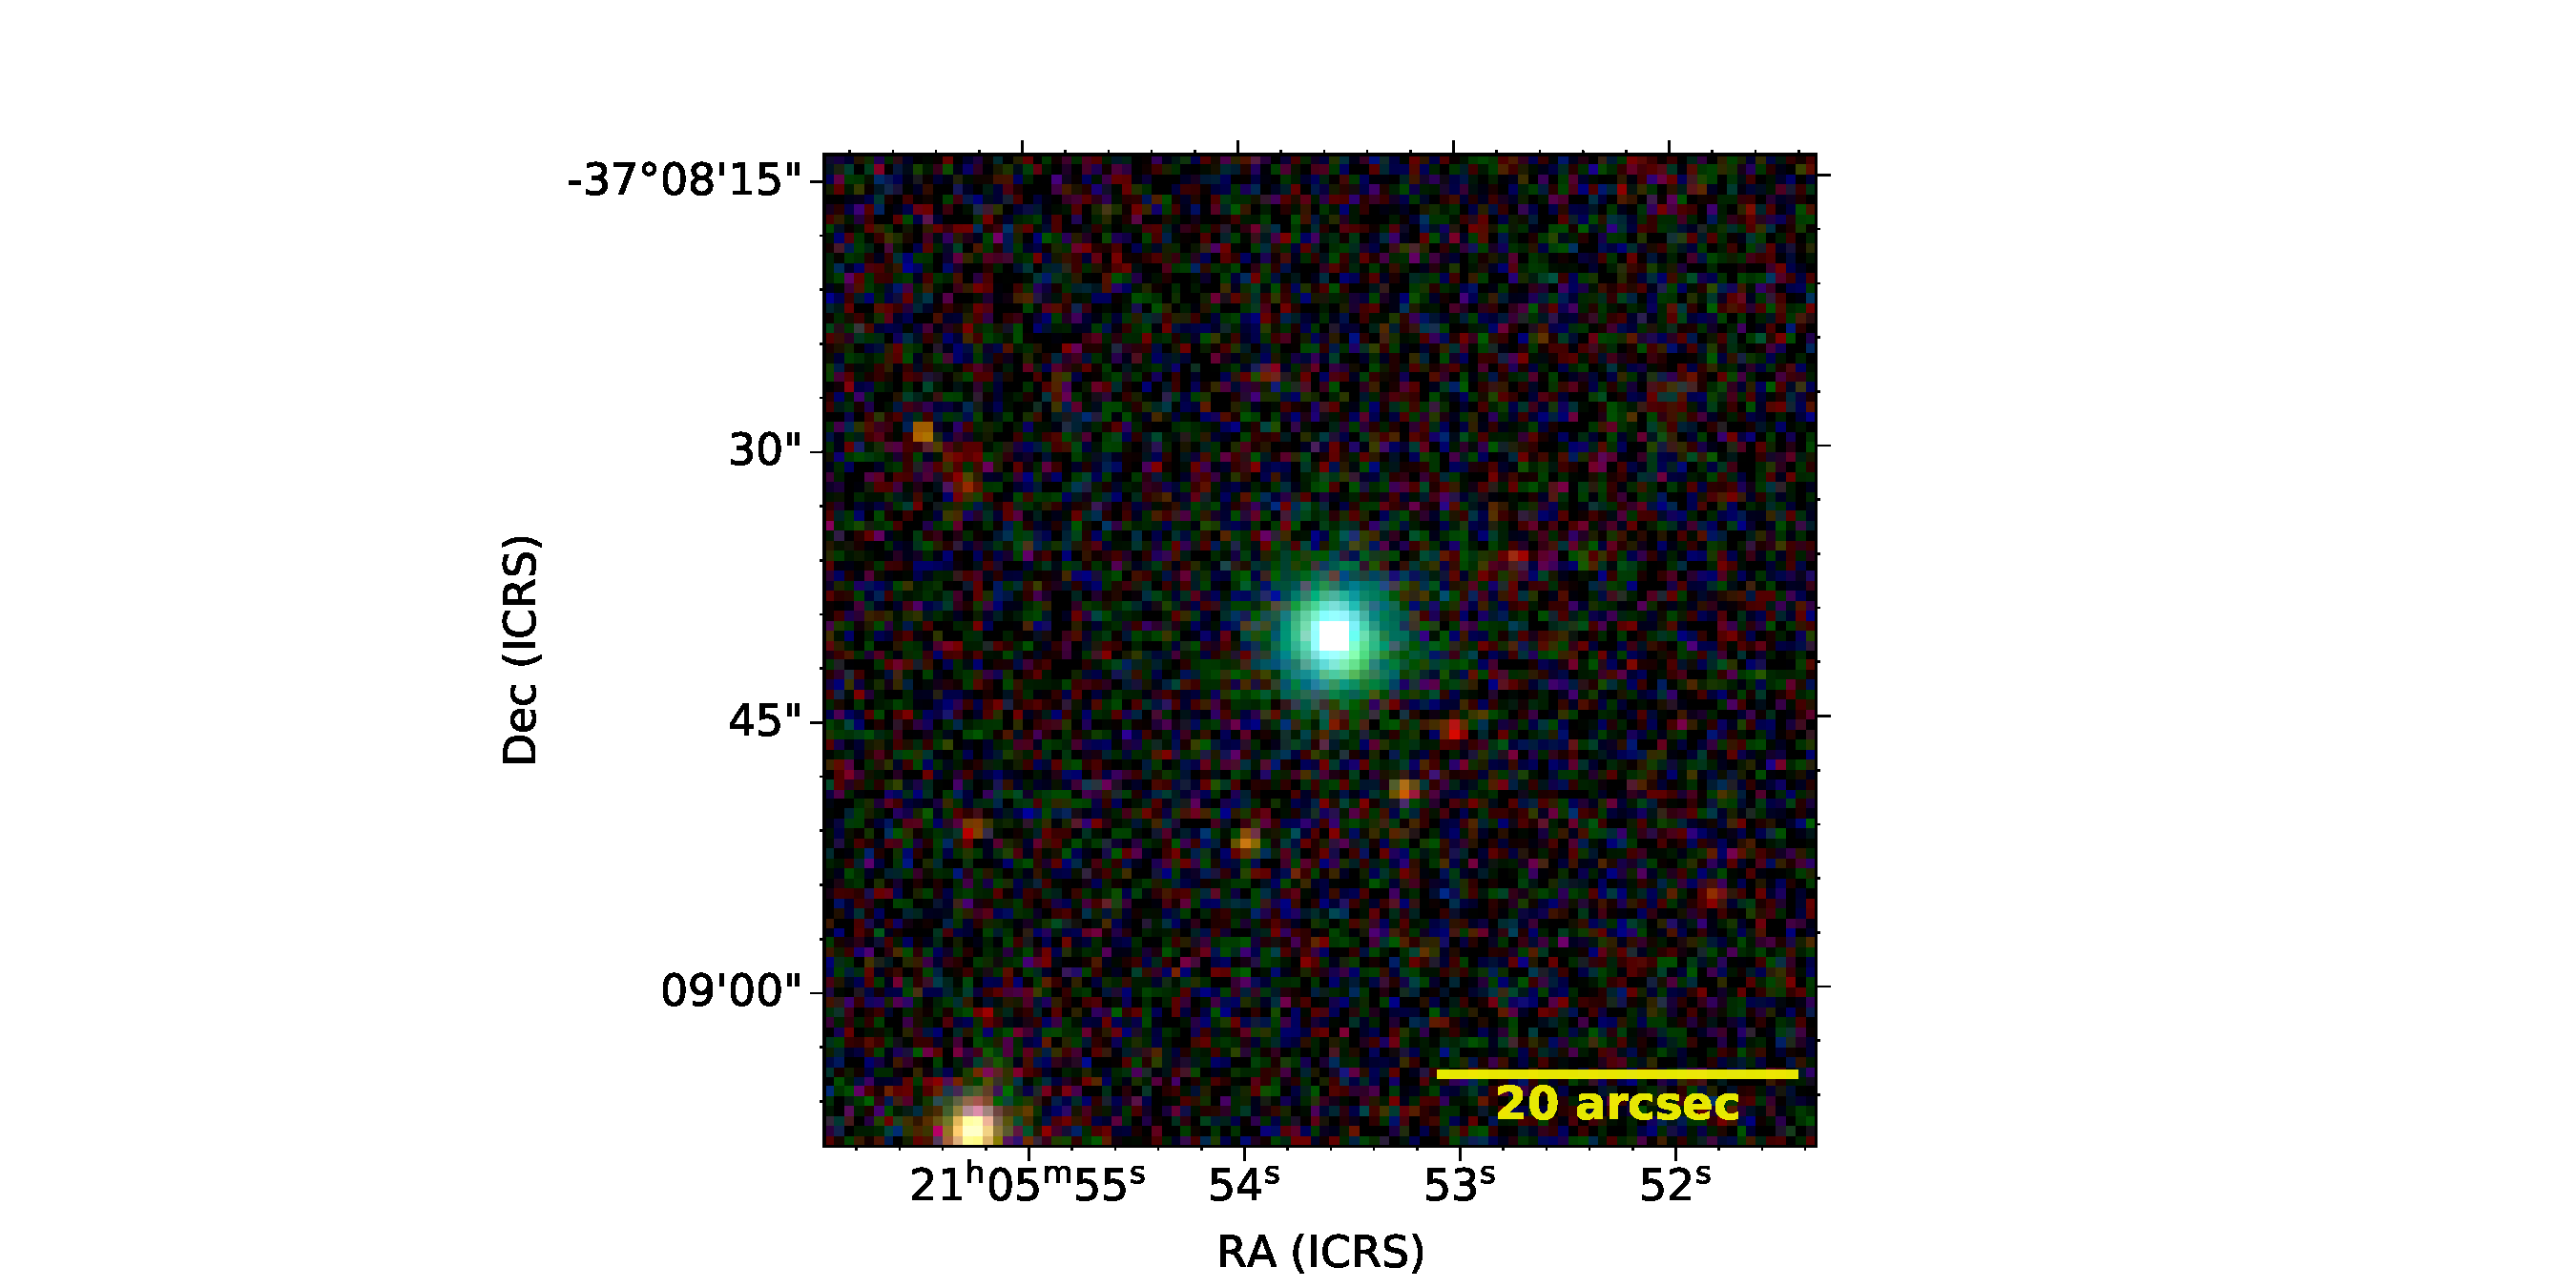
\includegraphics[width=0.3\linewidth, trim=10 0 65 20, clip]{Figs/PNG006_316-37_100_r.pdf} \\
     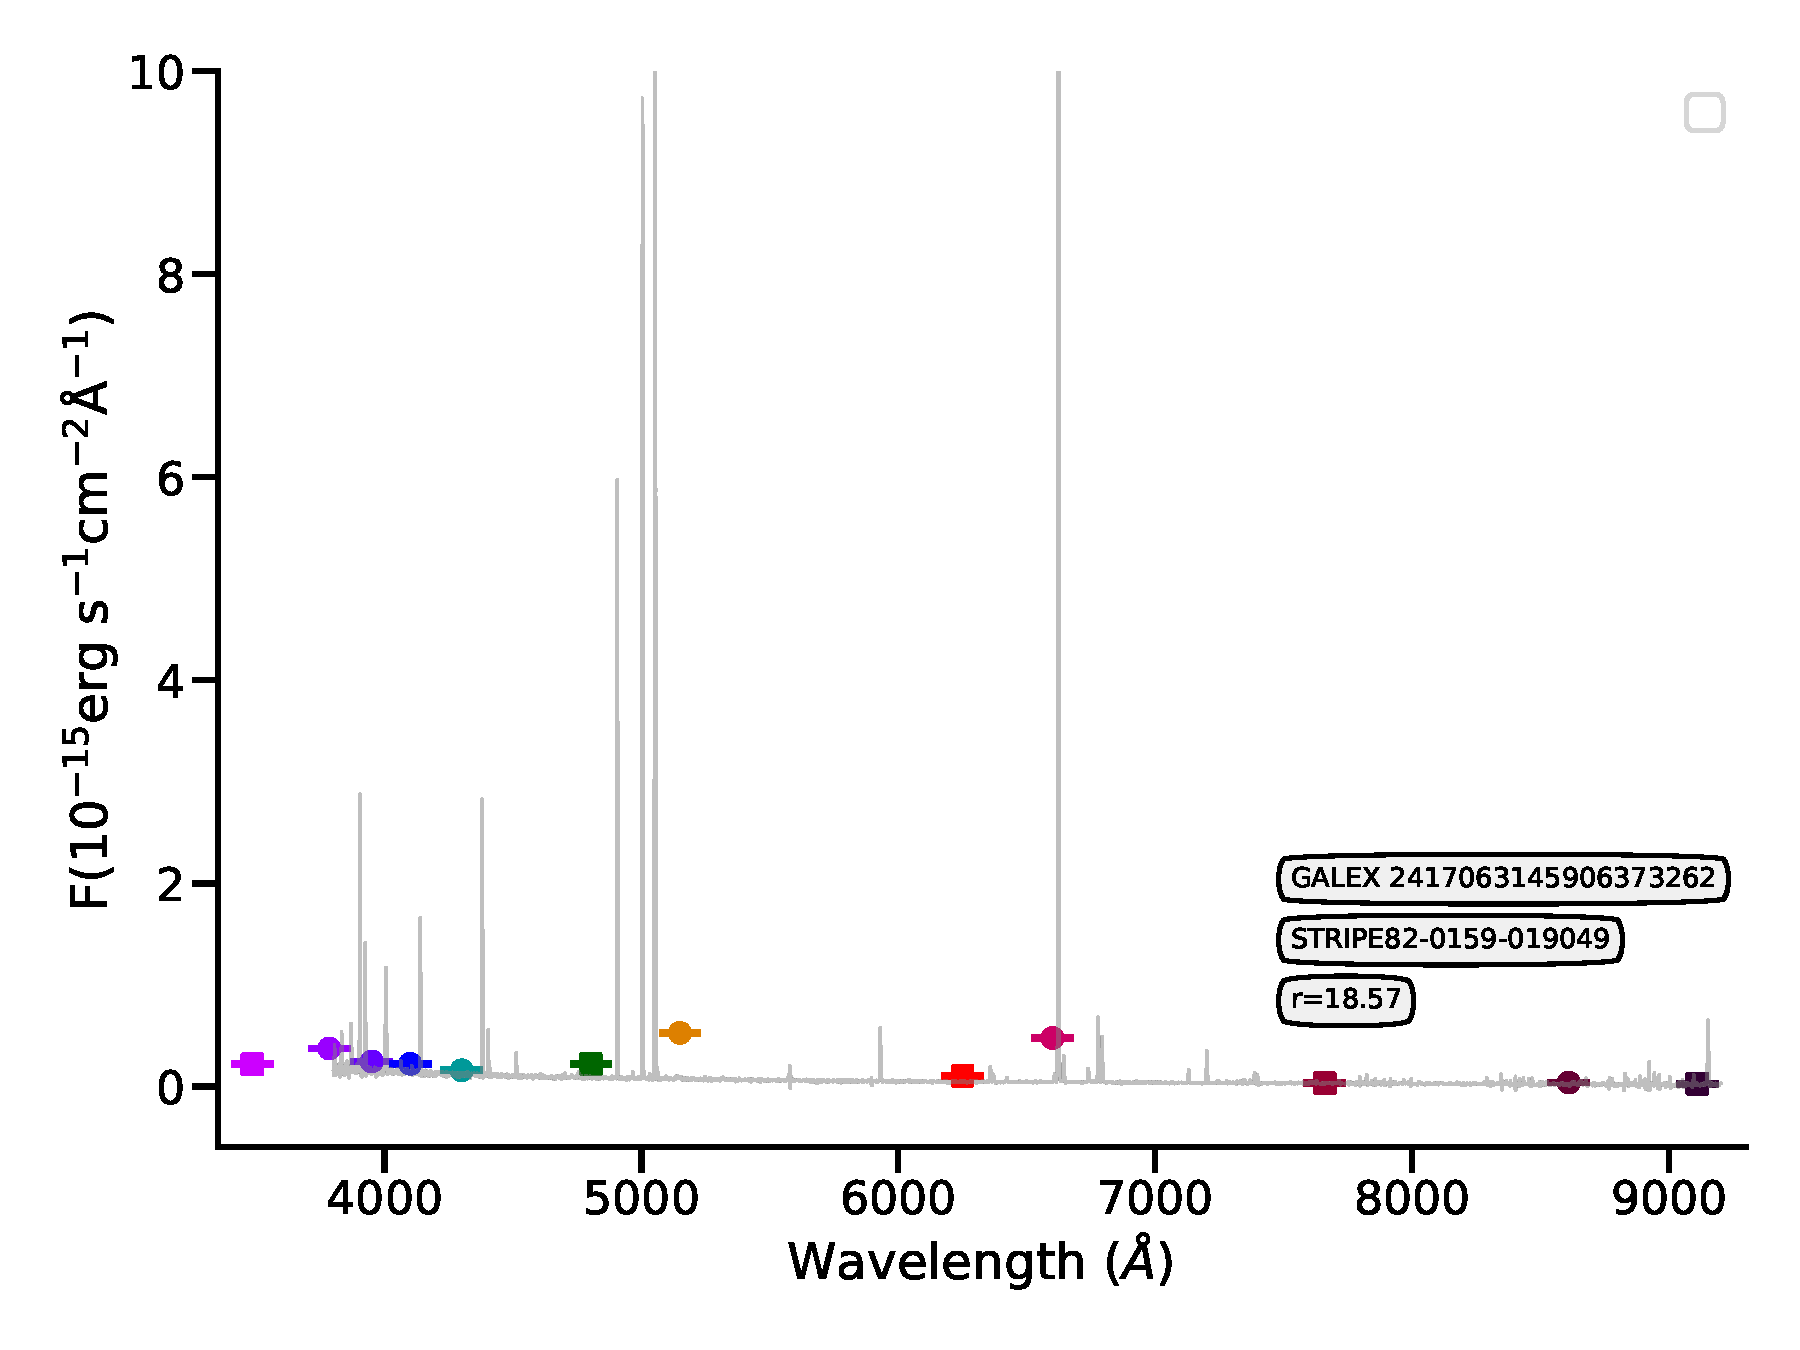
\includegraphics[trim=10 0 10 20, clip]{Figs/spec-0680-52200-0153-STRIPE82-0159-019049.pdf} & 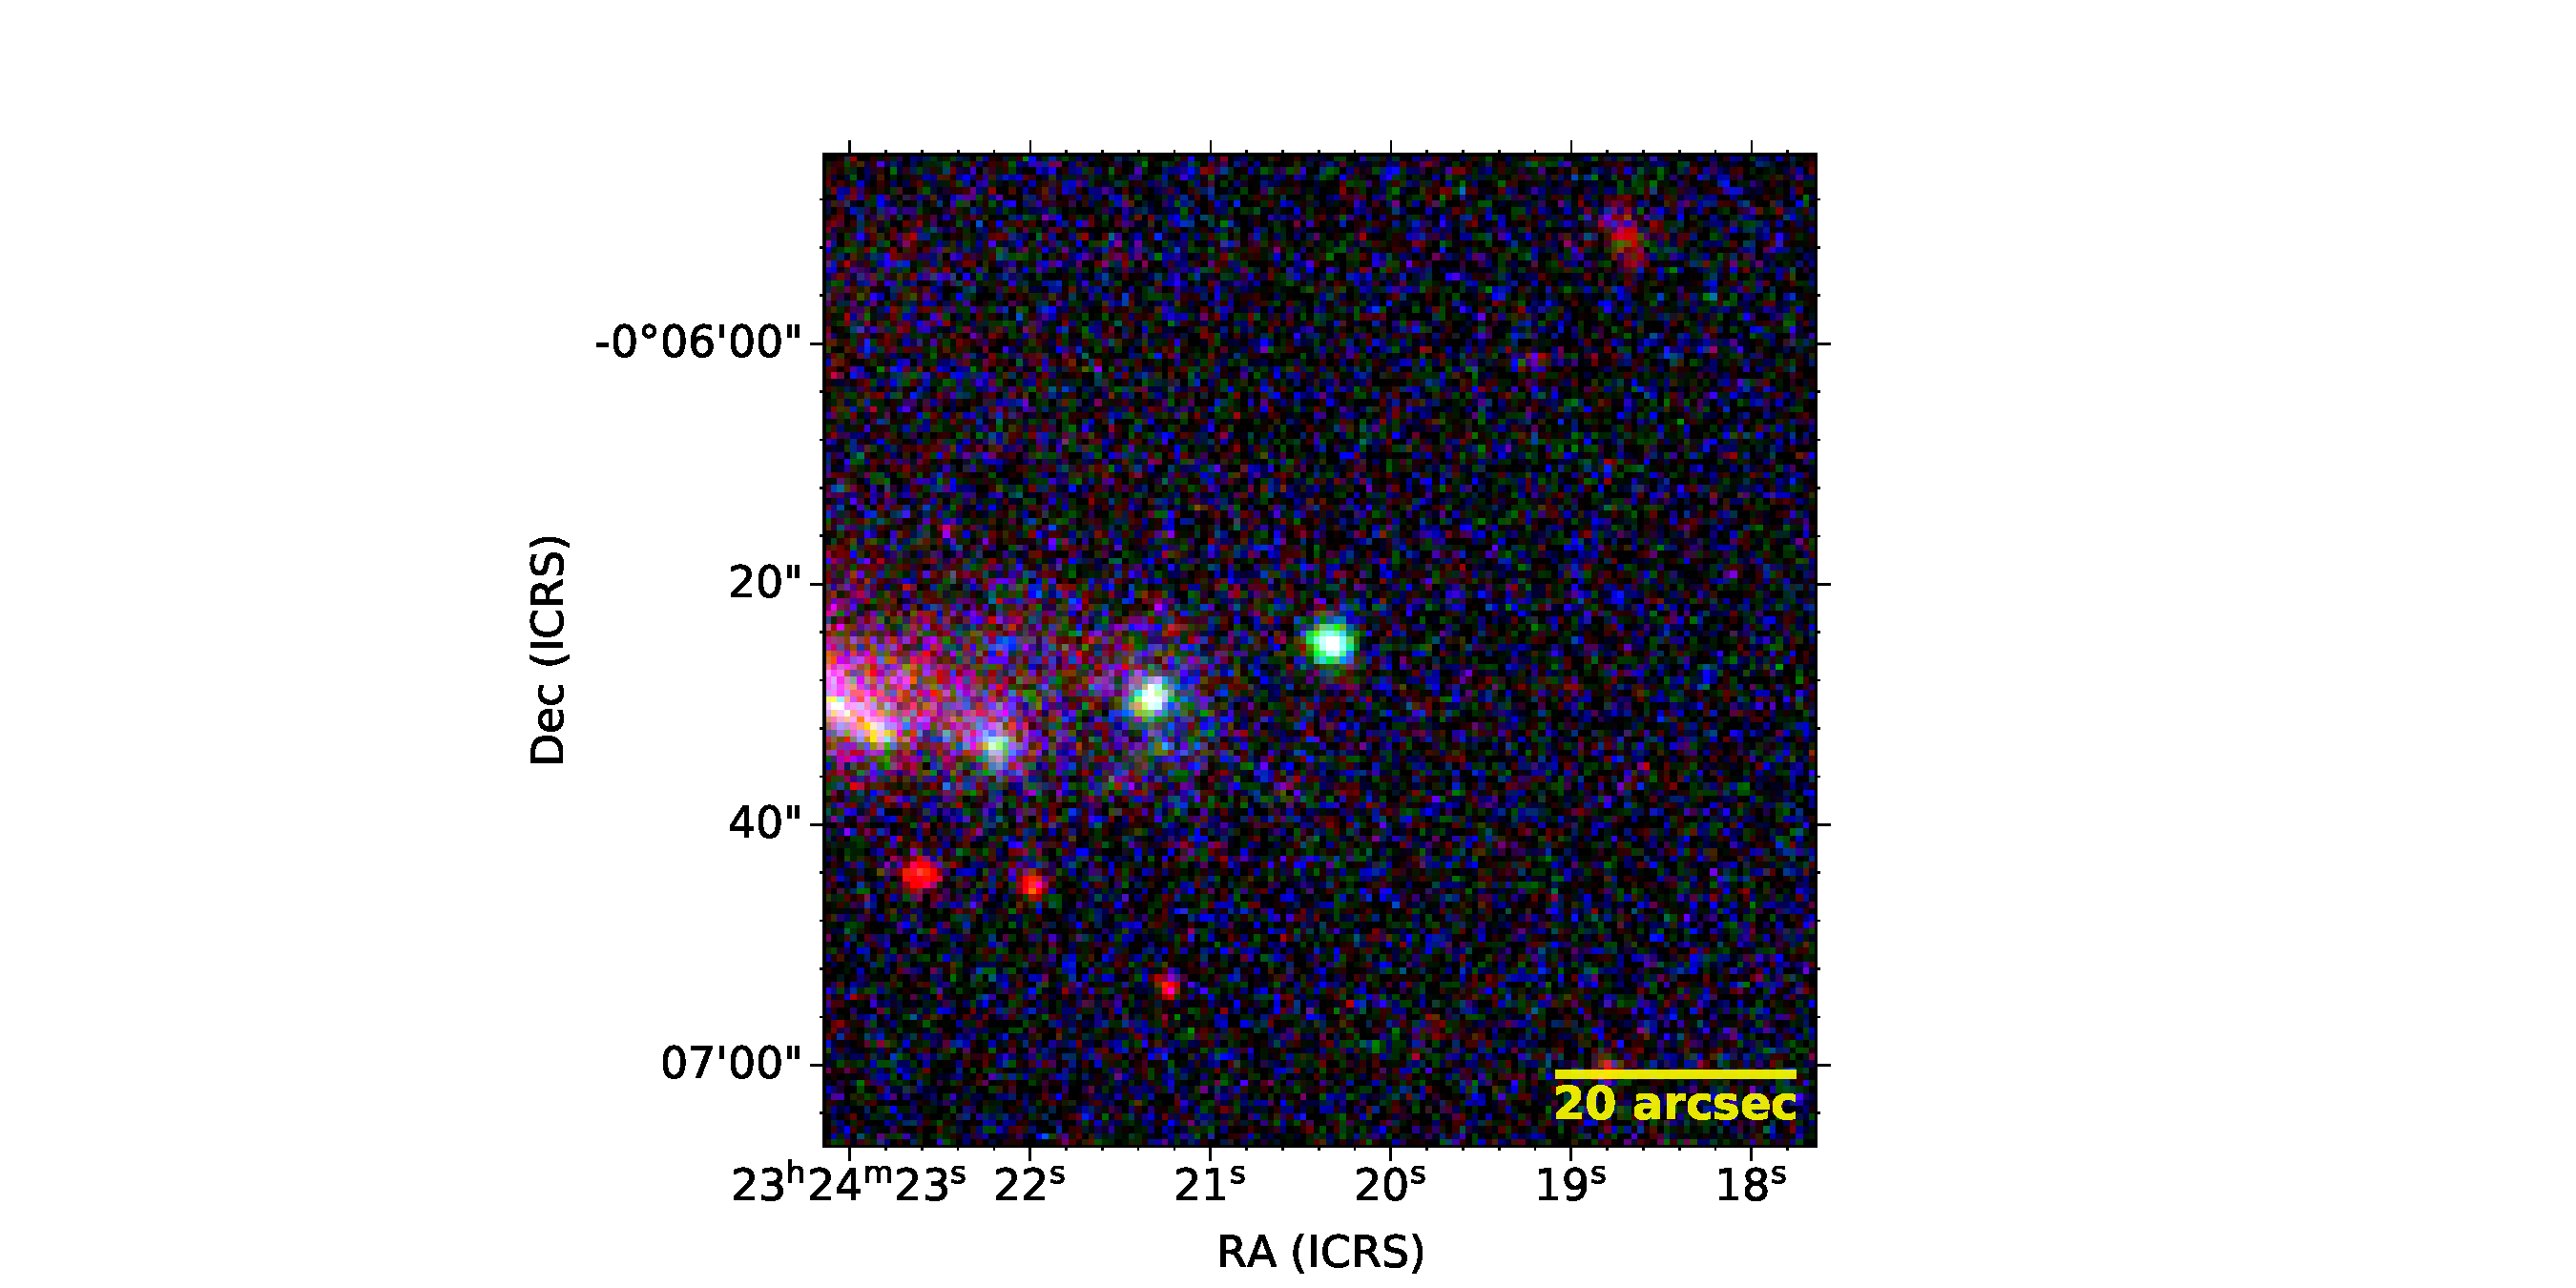
\includegraphics[width=0.3\linewidth, trim=10 0 65 20, clip]{Figs/GALEX24170_351-0_150_r.pdf} \\
    (c) & (d) \\
    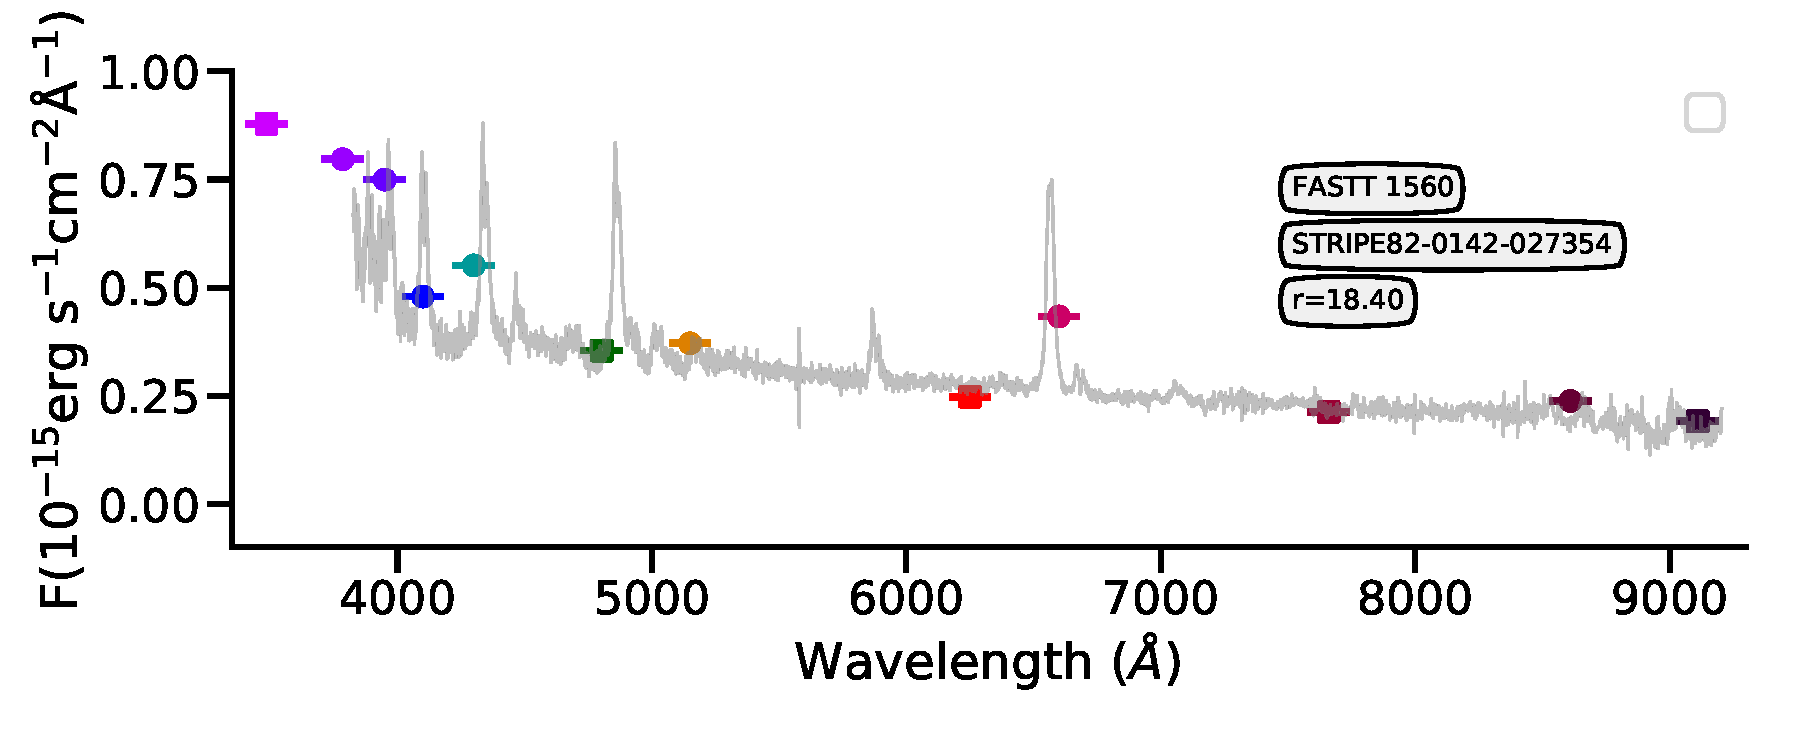
\includegraphics[trim=10 0 10 20, clip]{Figs/spec-0376-52143-0631-STRIPE82-0142-027354.pdf} & 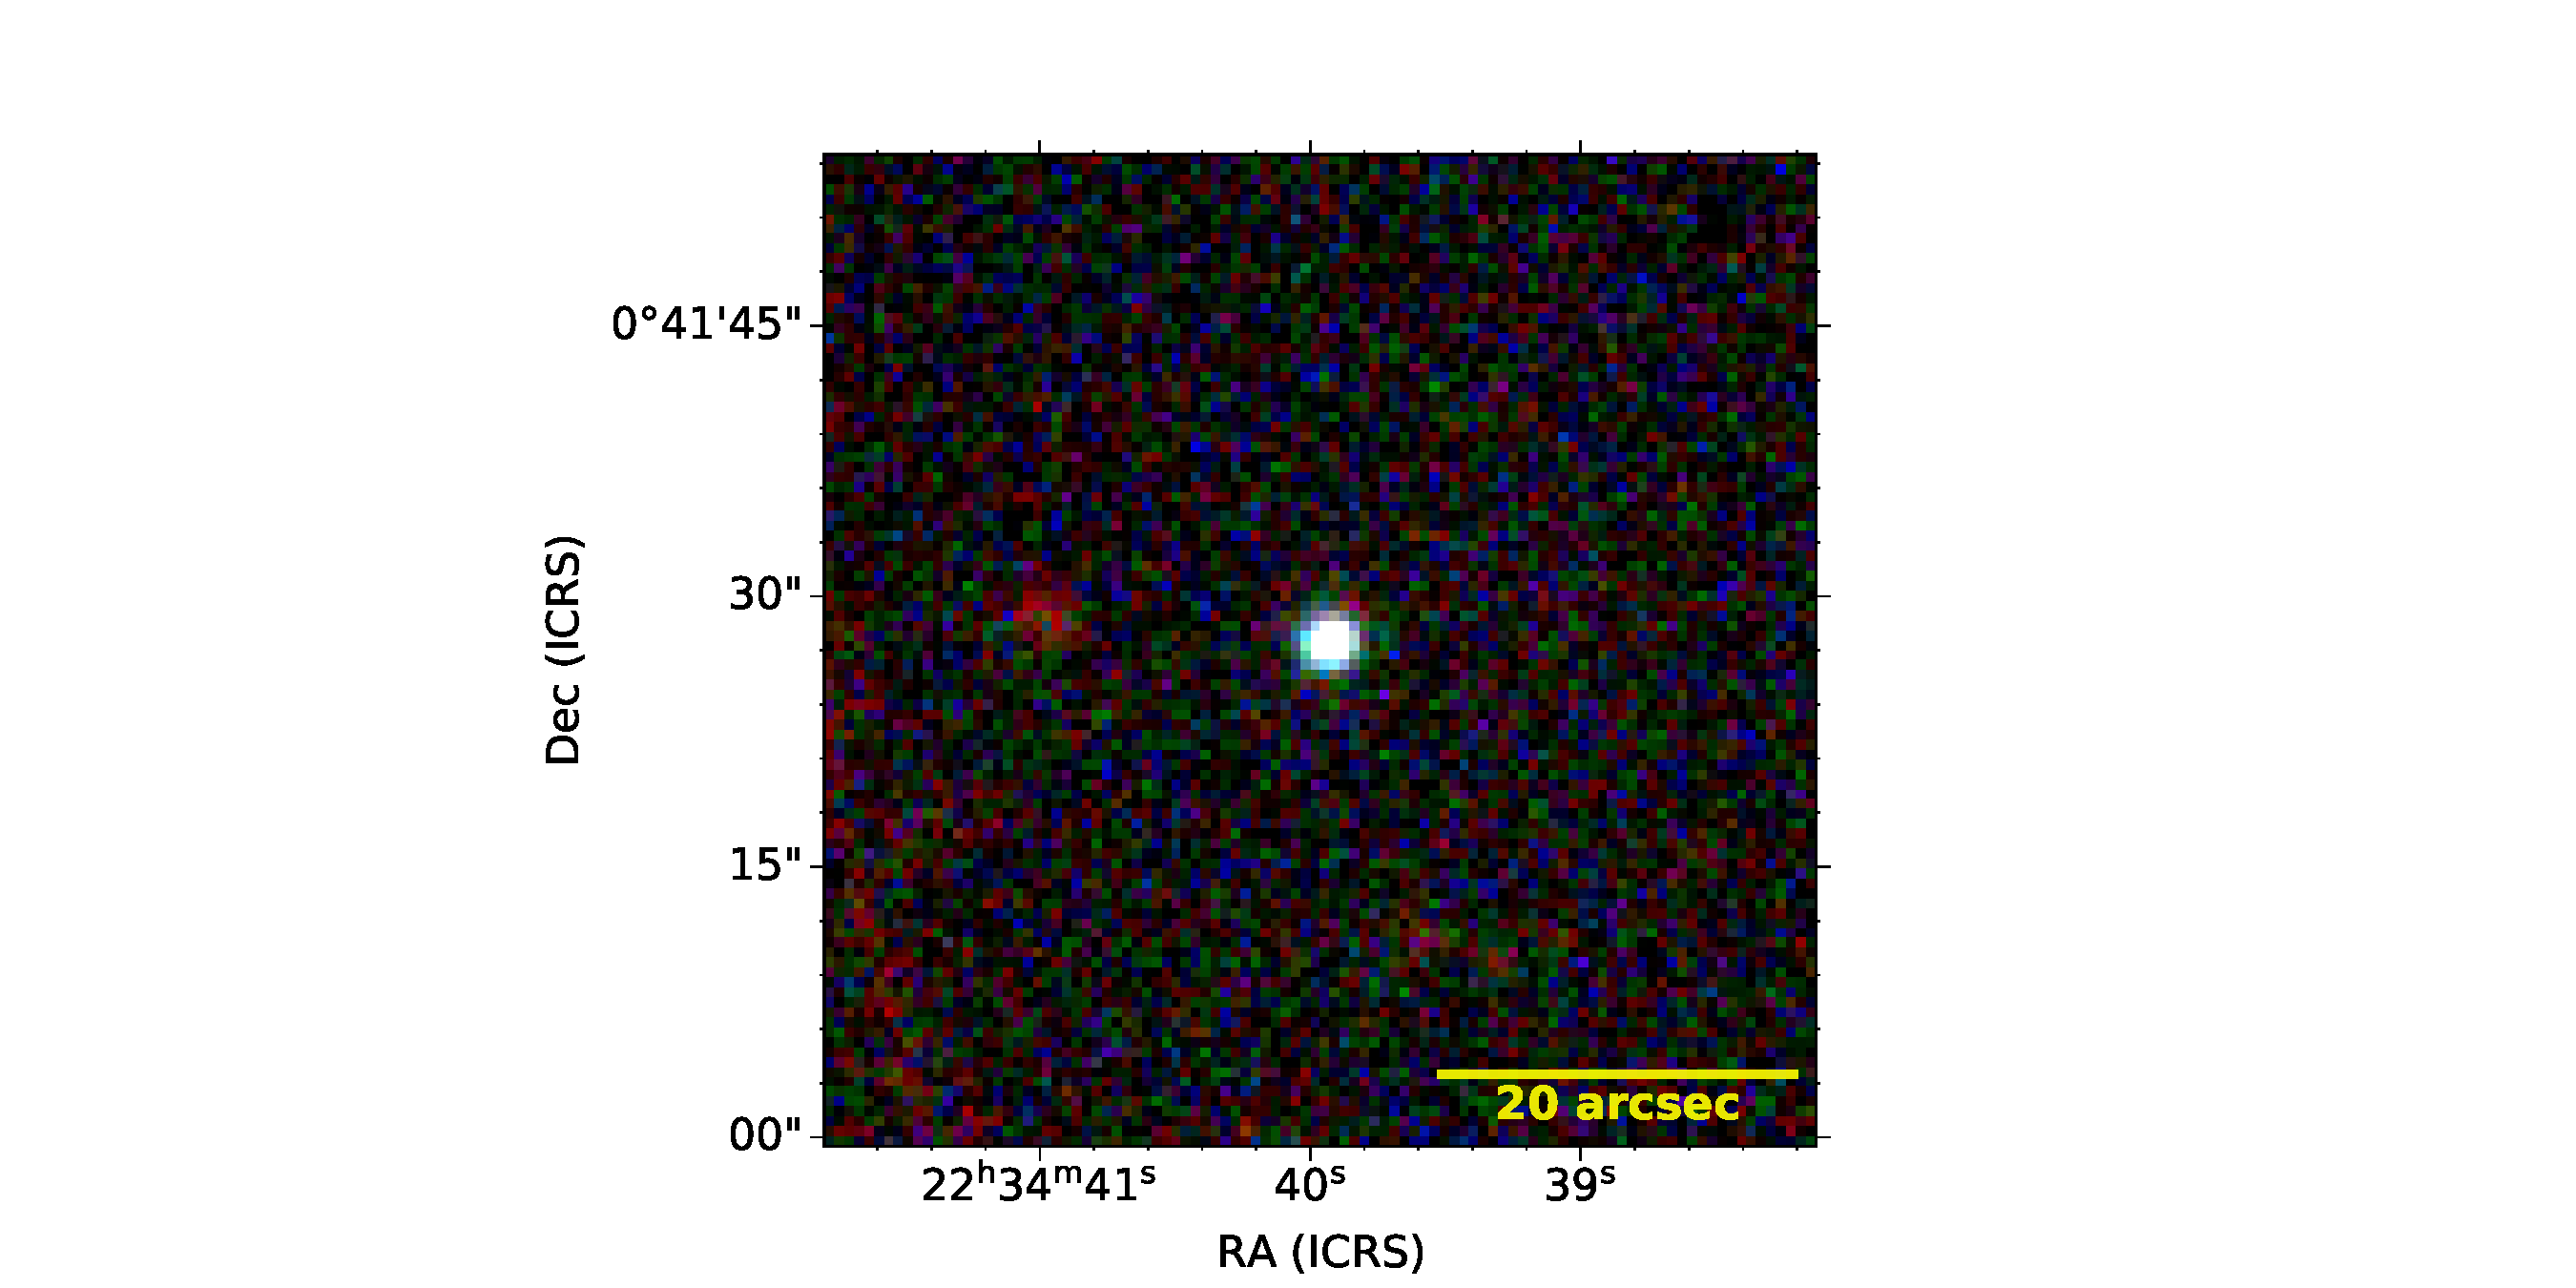
\includegraphics[width=0.3\linewidth, trim=10 0 65 20, clip]{Figs/FASTT1560_338-0_100_r.pdf} \\
     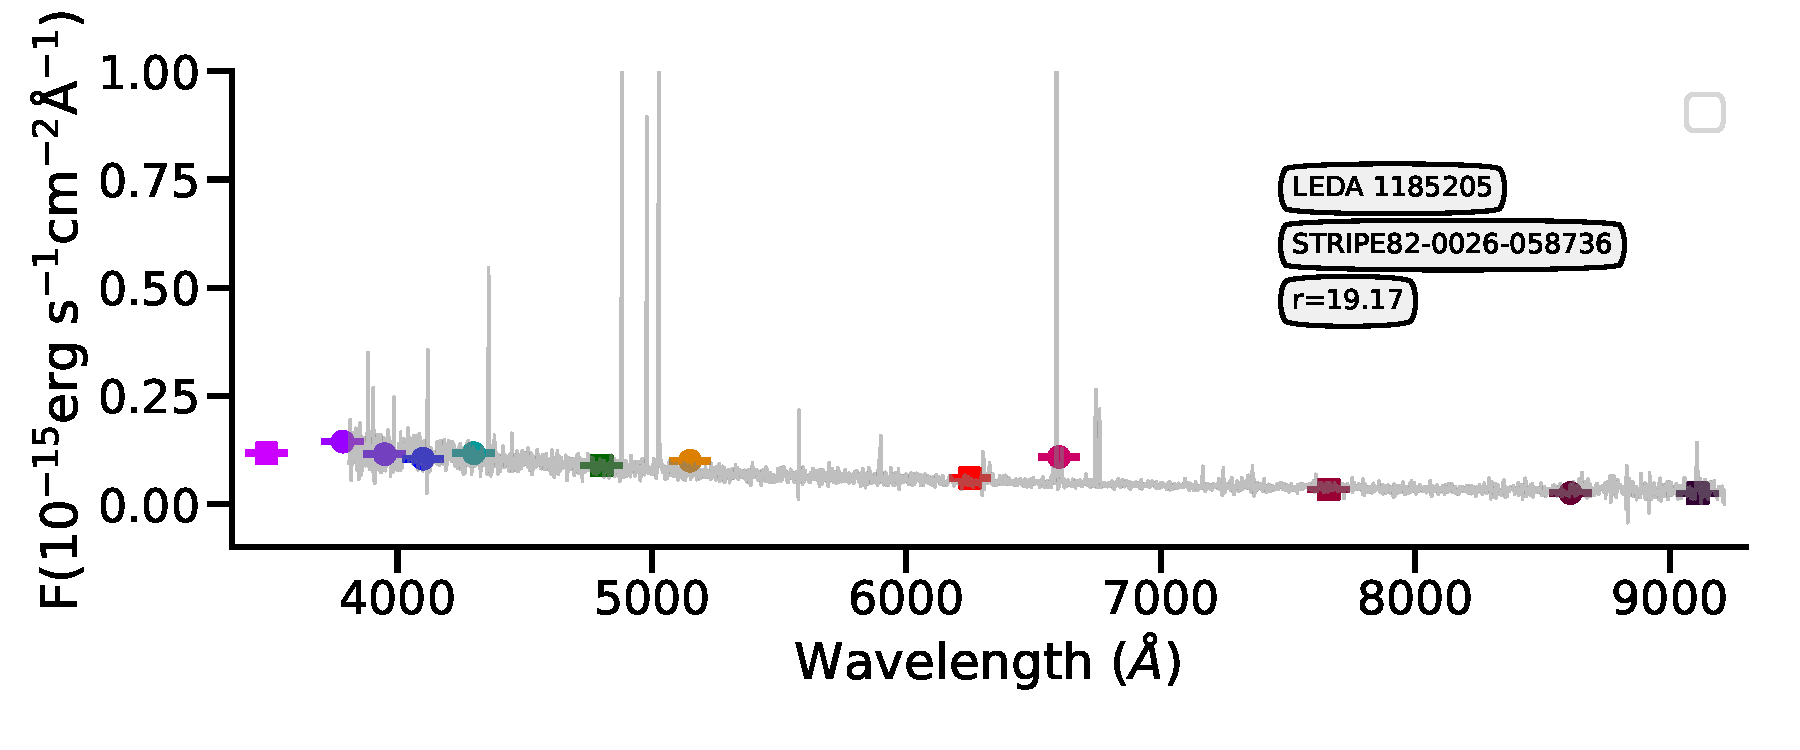
\includegraphics[trim=10 0 10 20, clip]{Figs/spec-0397-51794-0336-STRIPE82-0026-058736.pdf} & 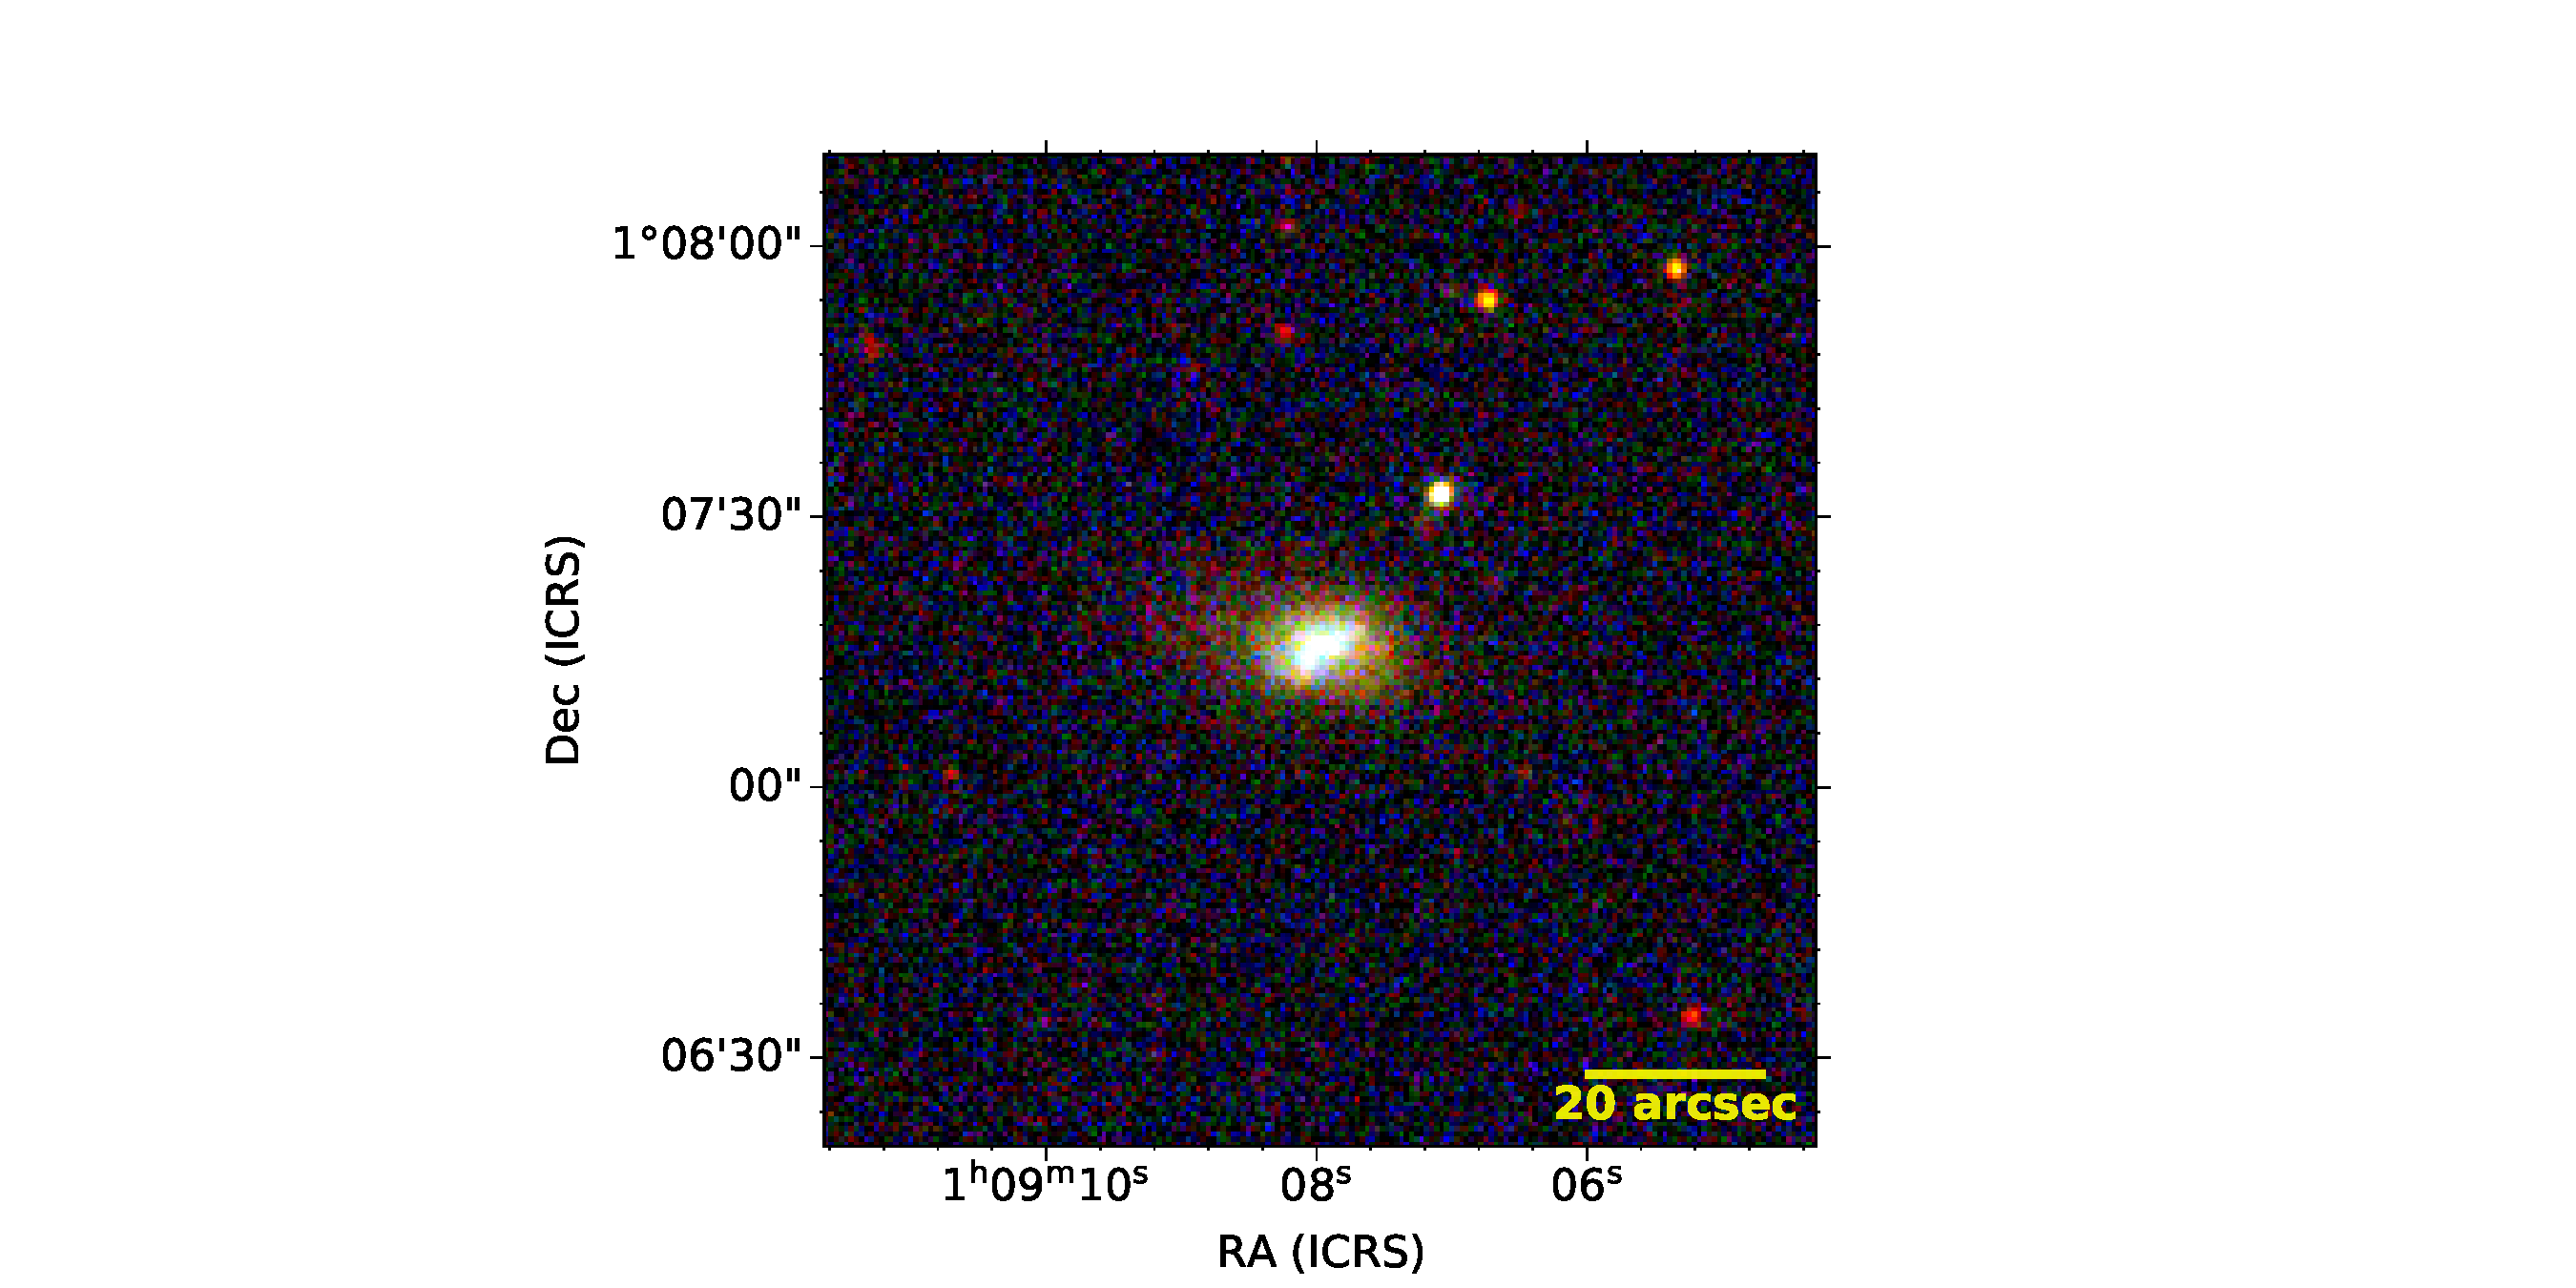
\includegraphics[width=0.3\linewidth, trim=10 0 65 20, clip]{Figs/LEDA1185205_17-1_200_r.pdf} \\
     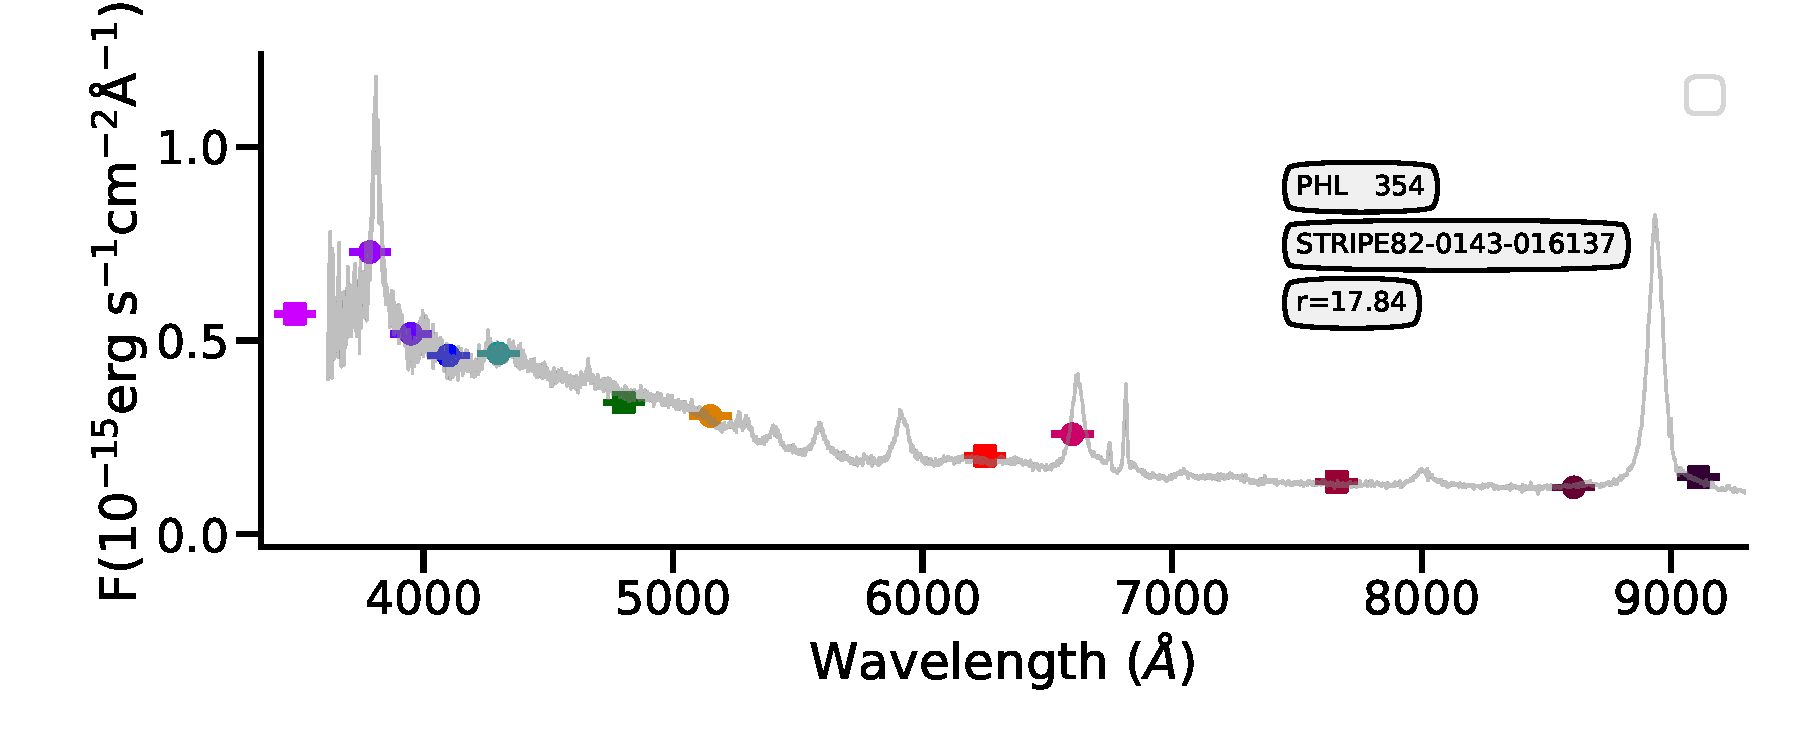
\includegraphics[trim=10 0 10 20, clip]{Figs/spec-9217-57934-0839-STRIPE82-0143-016137.pdf} & 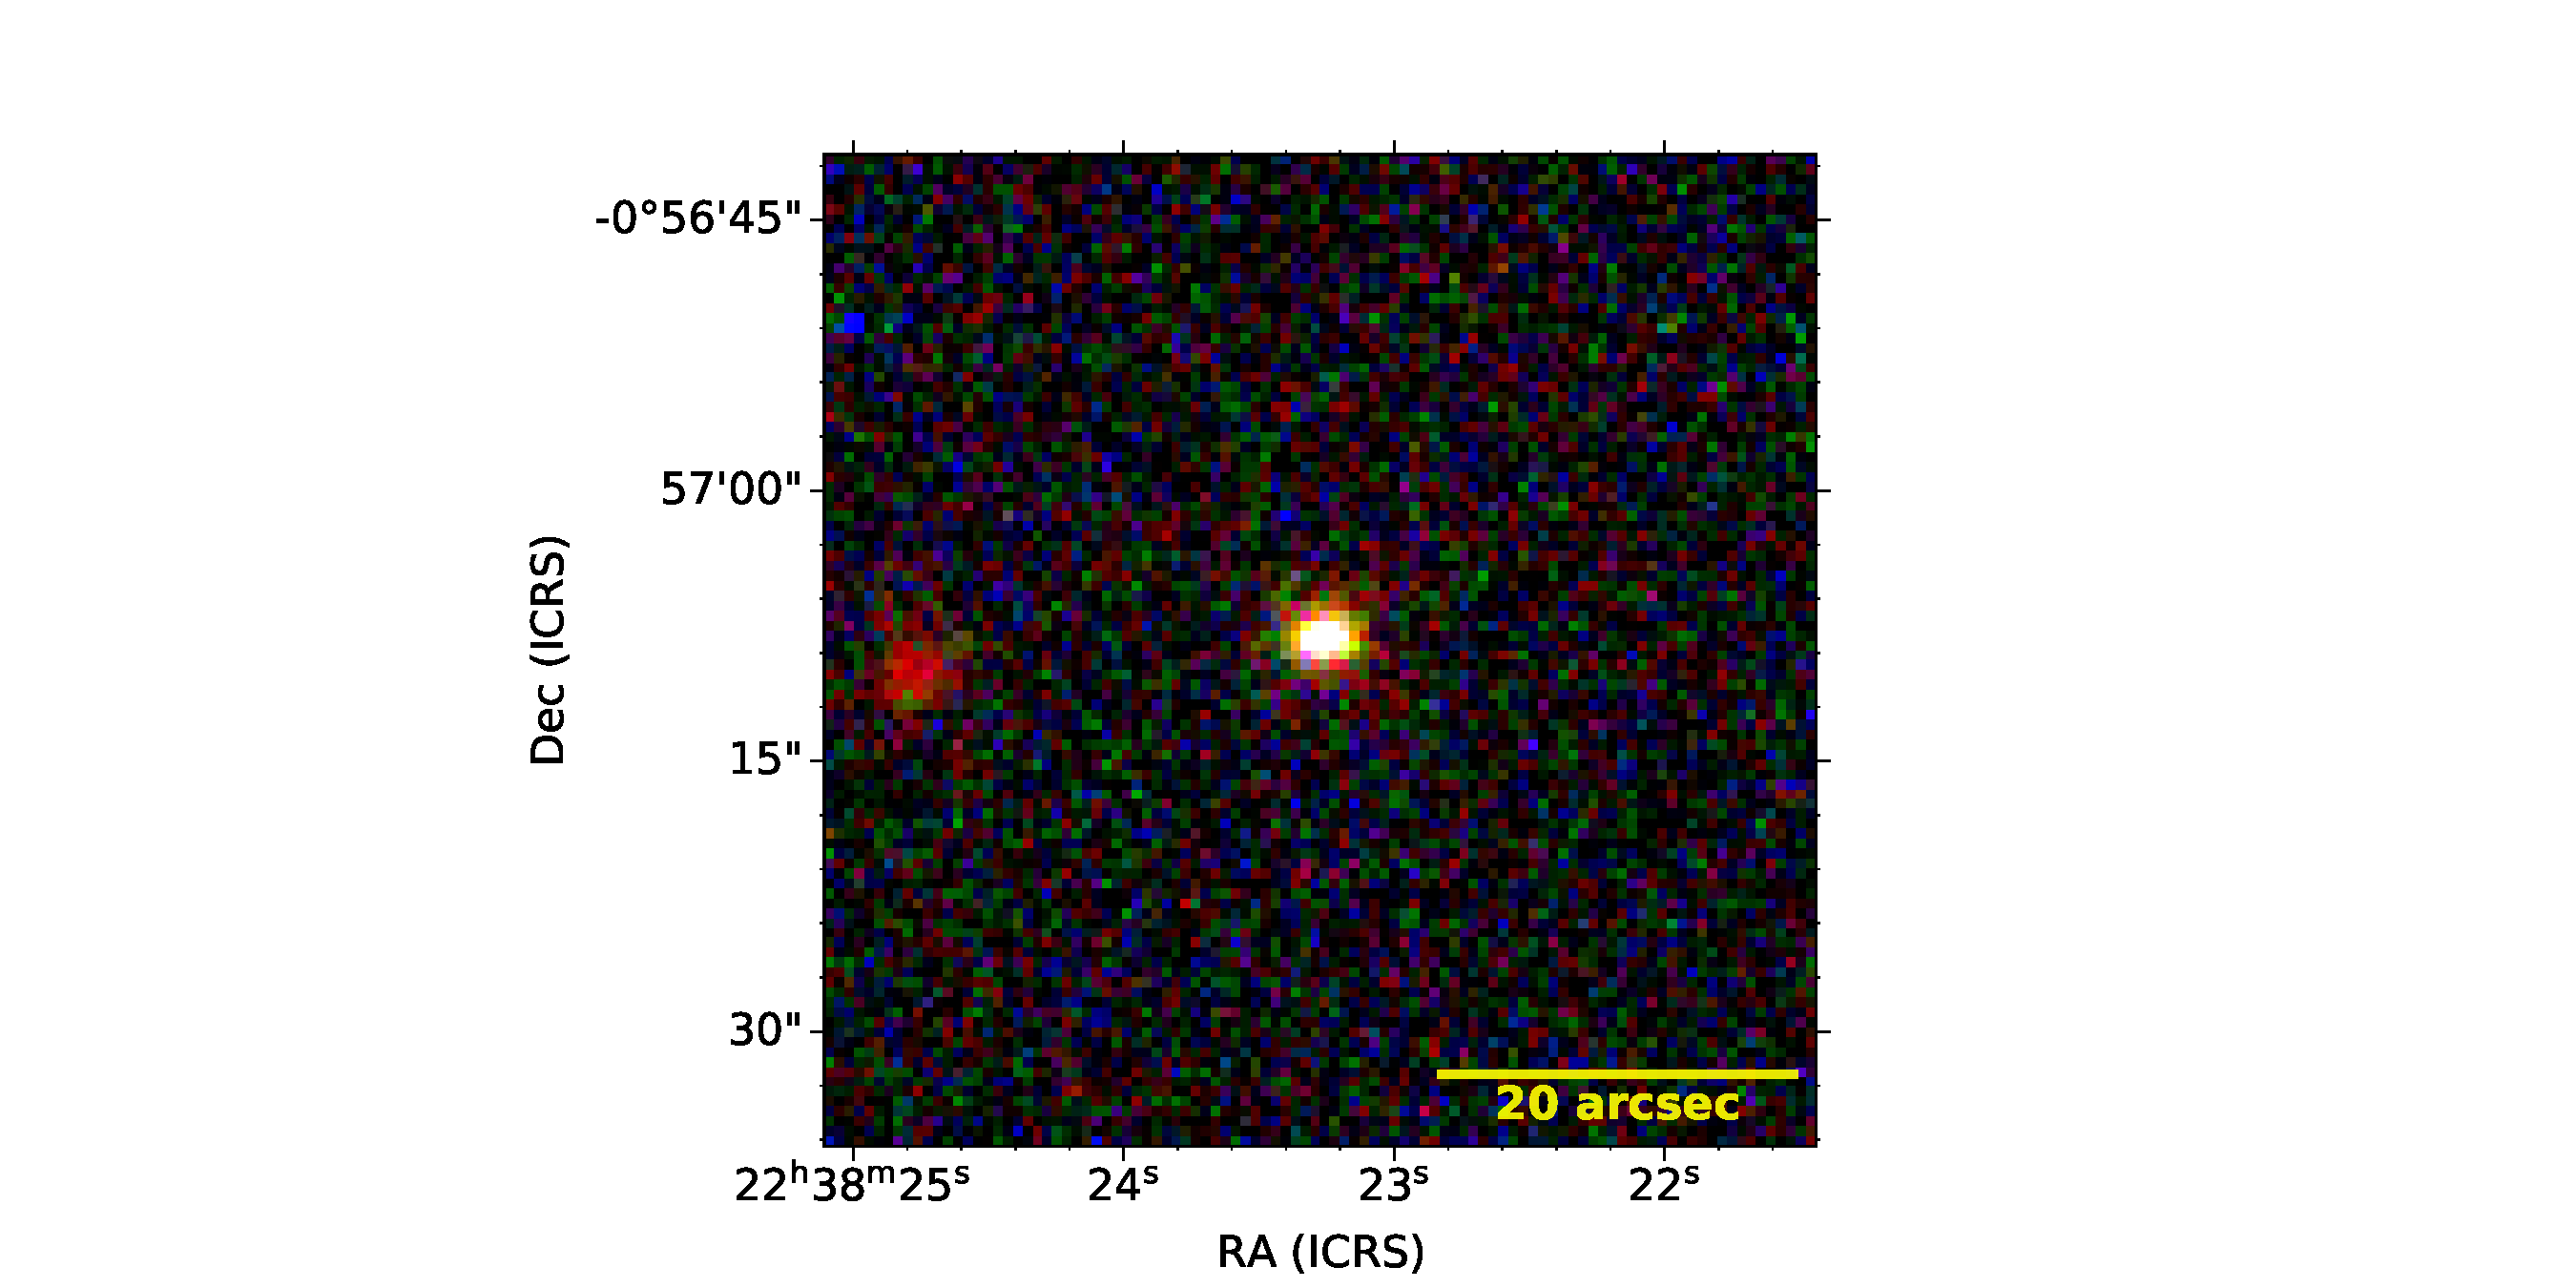
\includegraphics[width=0.3\linewidth, trim=10 0 65 20, clip]{Figs/PHL354_339-0_100_r.pdf} \\
  \end{tabular}
  \caption{Spectra of the known objects select with our algorithm }
  \label{fig:color-diagram}
\end{figure*}

\begin{figure*}
  \setlength\tabcolsep{0pt}
  \setkeys{Gin}{width=0.5\linewidth}
  \begin{tabular}{ll}
    (a) & (b) \\
    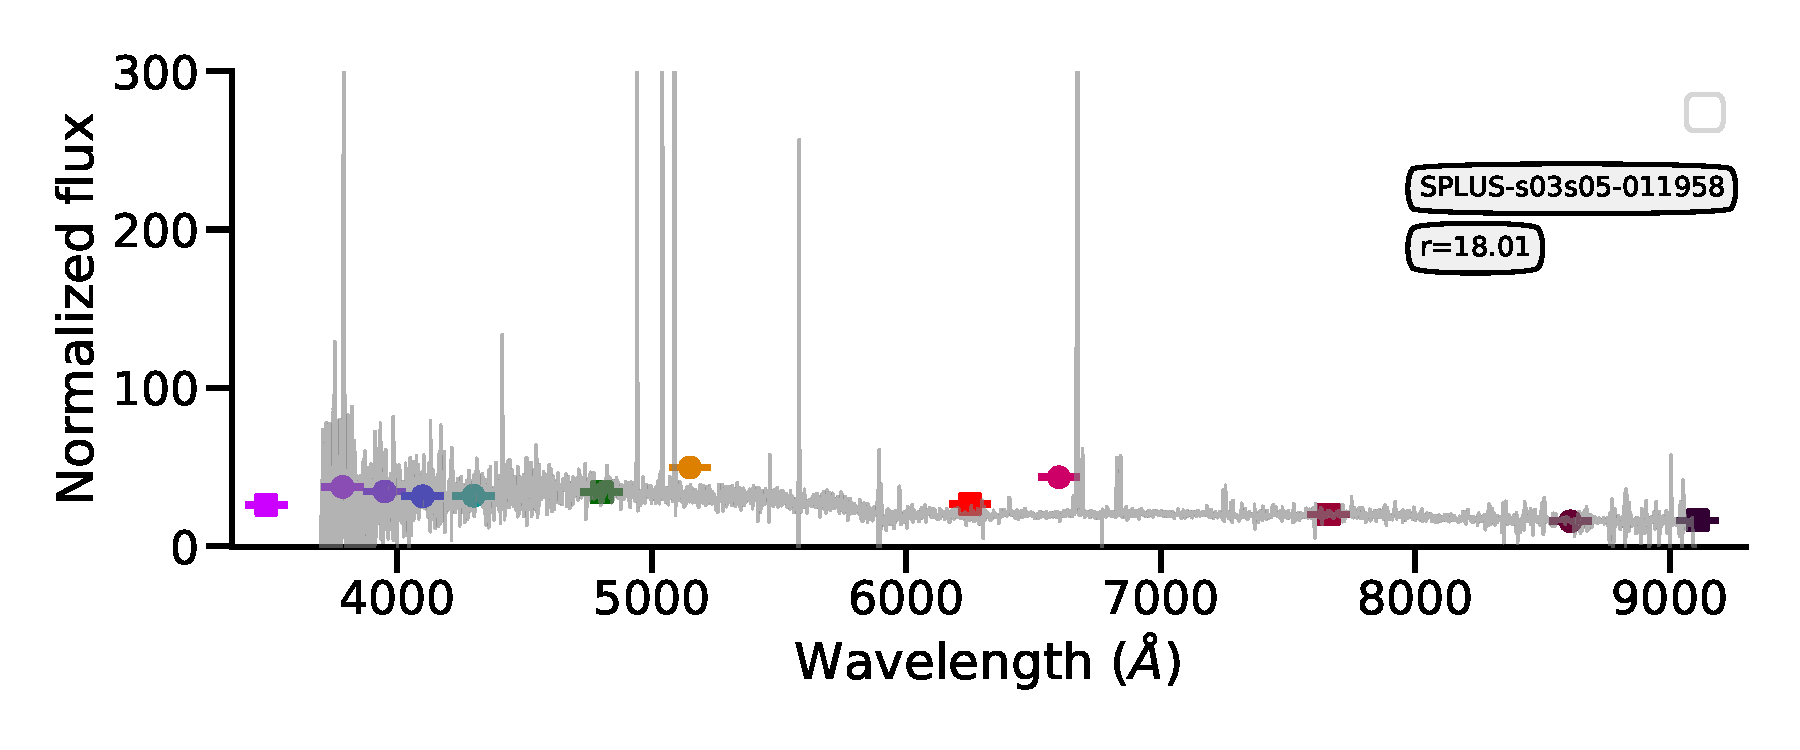
\includegraphics[trim=10 0 10 20, clip]{Figs/spec-57313-EG220318S020919M01_sp10-173-SPLUS-s03s05-011958.pdf} & 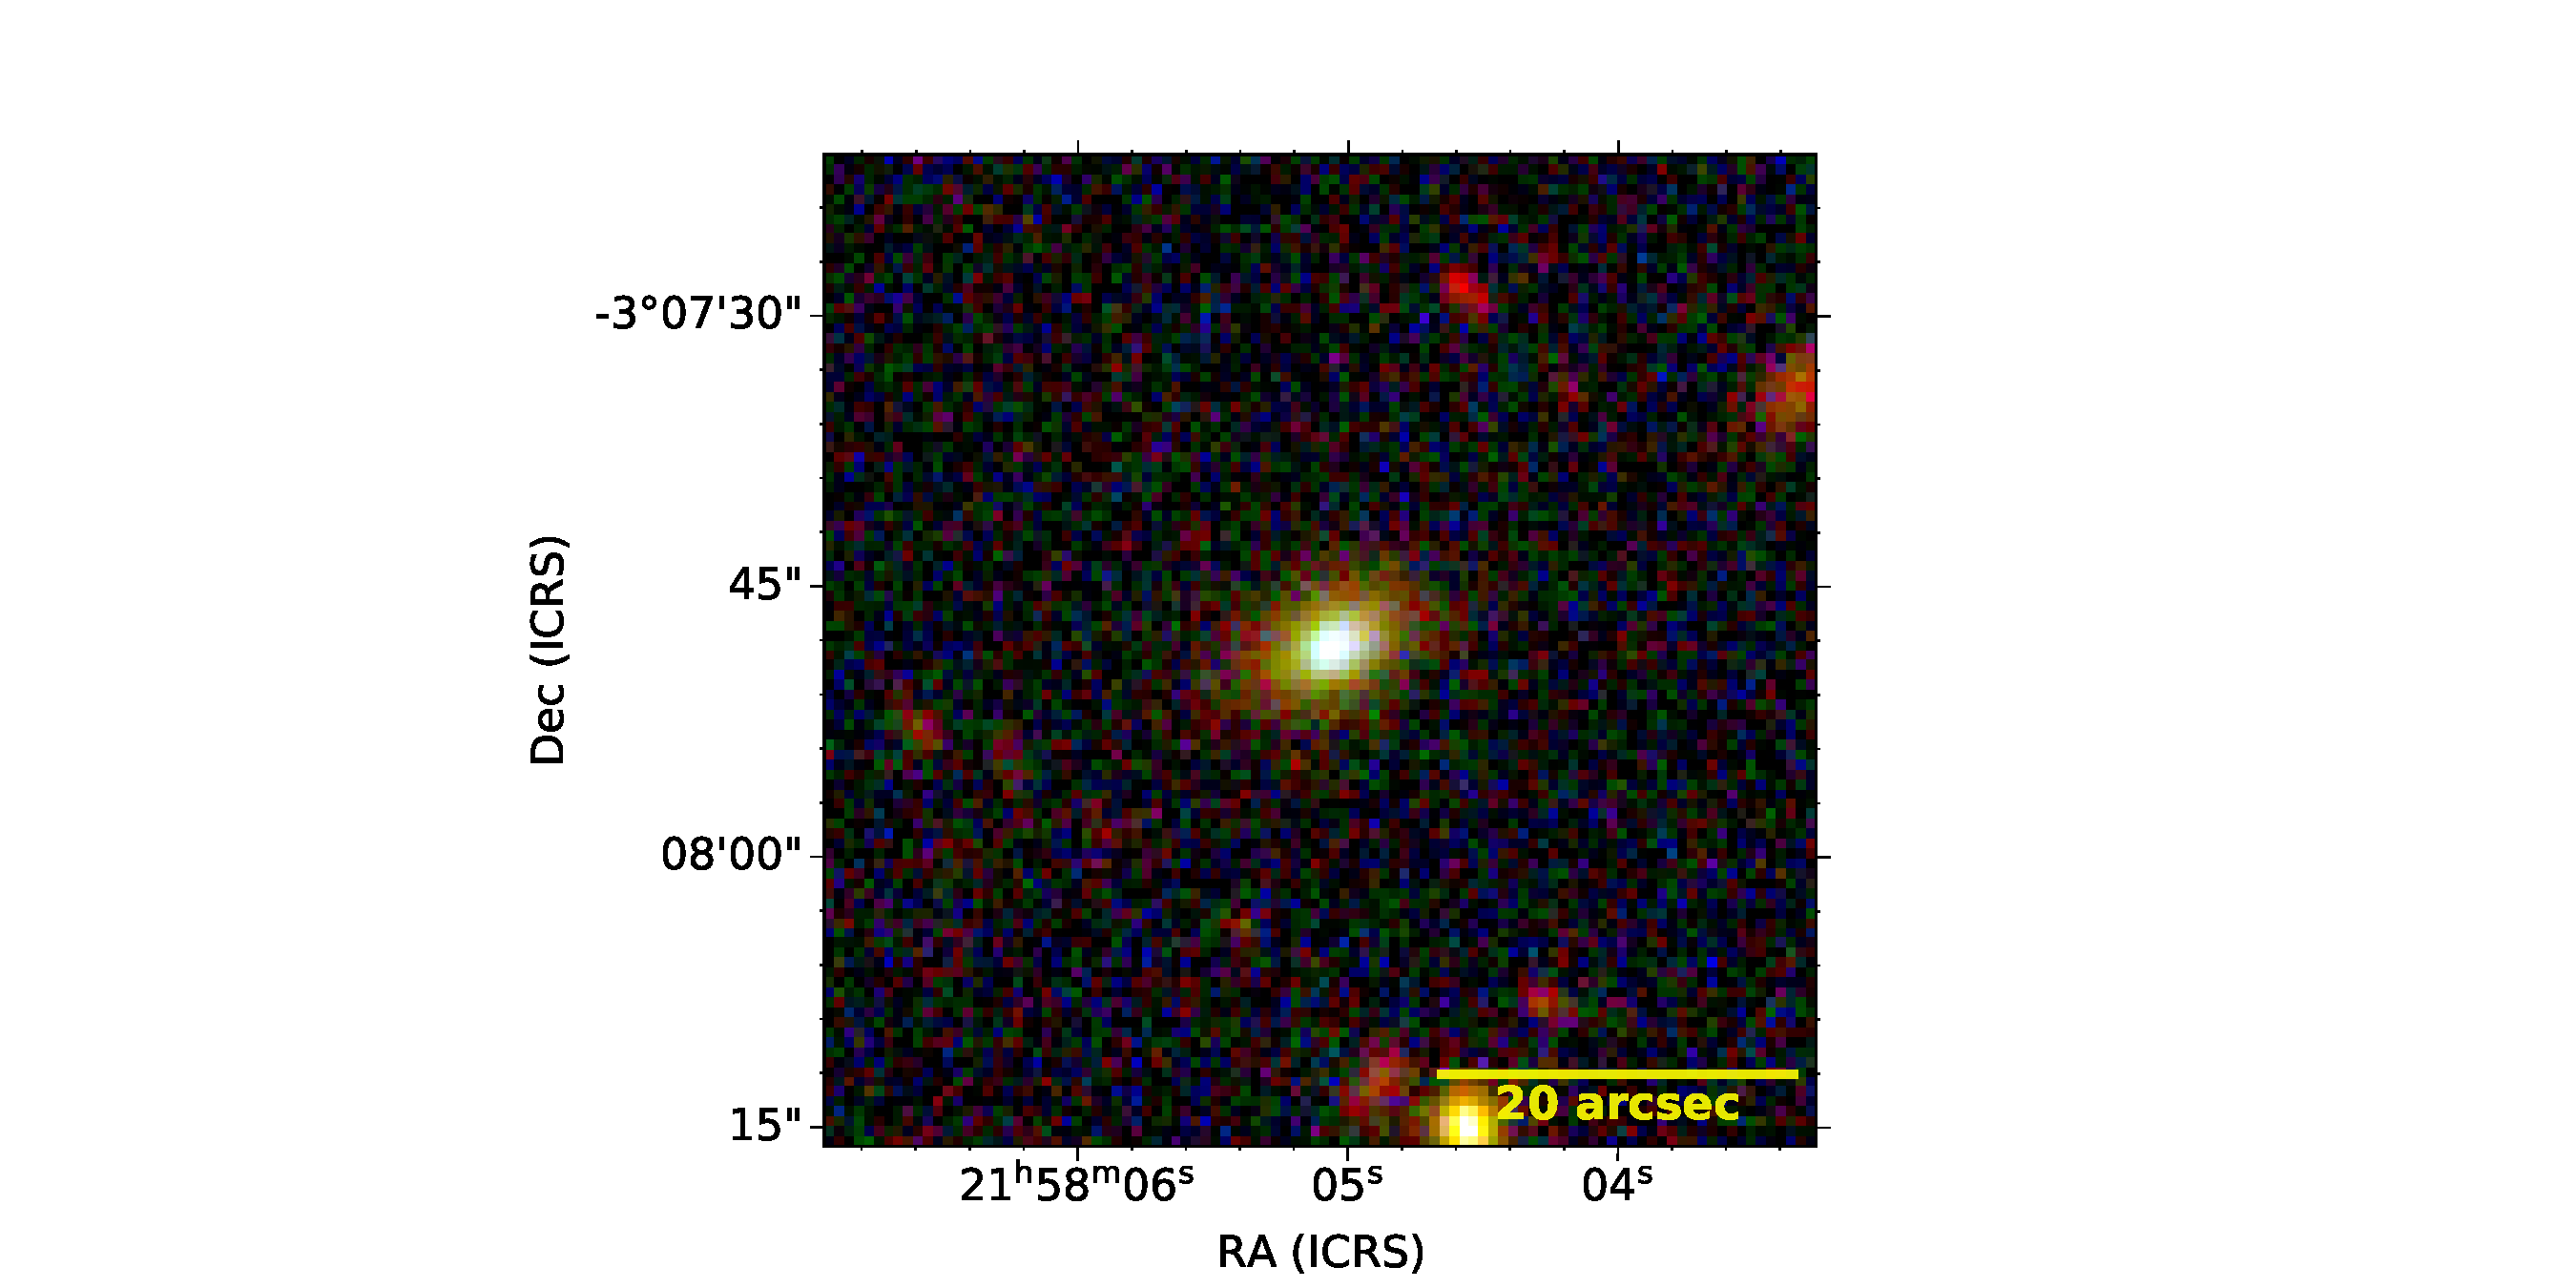
\includegraphics[width=0.3\linewidth, trim=10 0 65 20, clip]{Figs/SPLUS-s03s05-011958_329-3_100_r.pdf} \\
     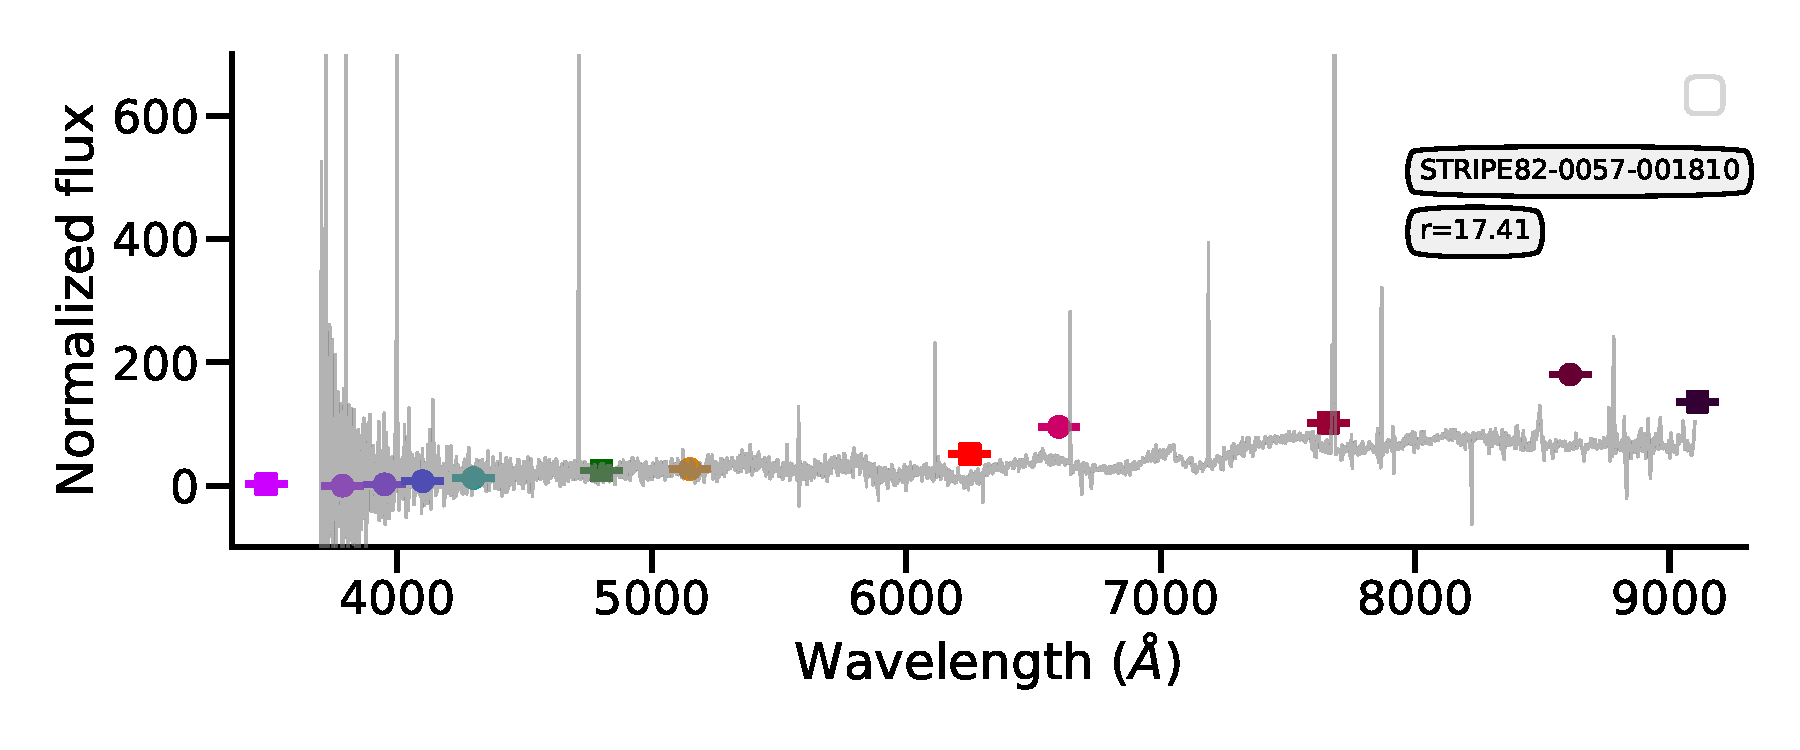
\includegraphics[trim=10 0 10 20, clip]{Figs/spec-55893-F9304_sp15-198-STRIPE82-0057-001810.pdf} & 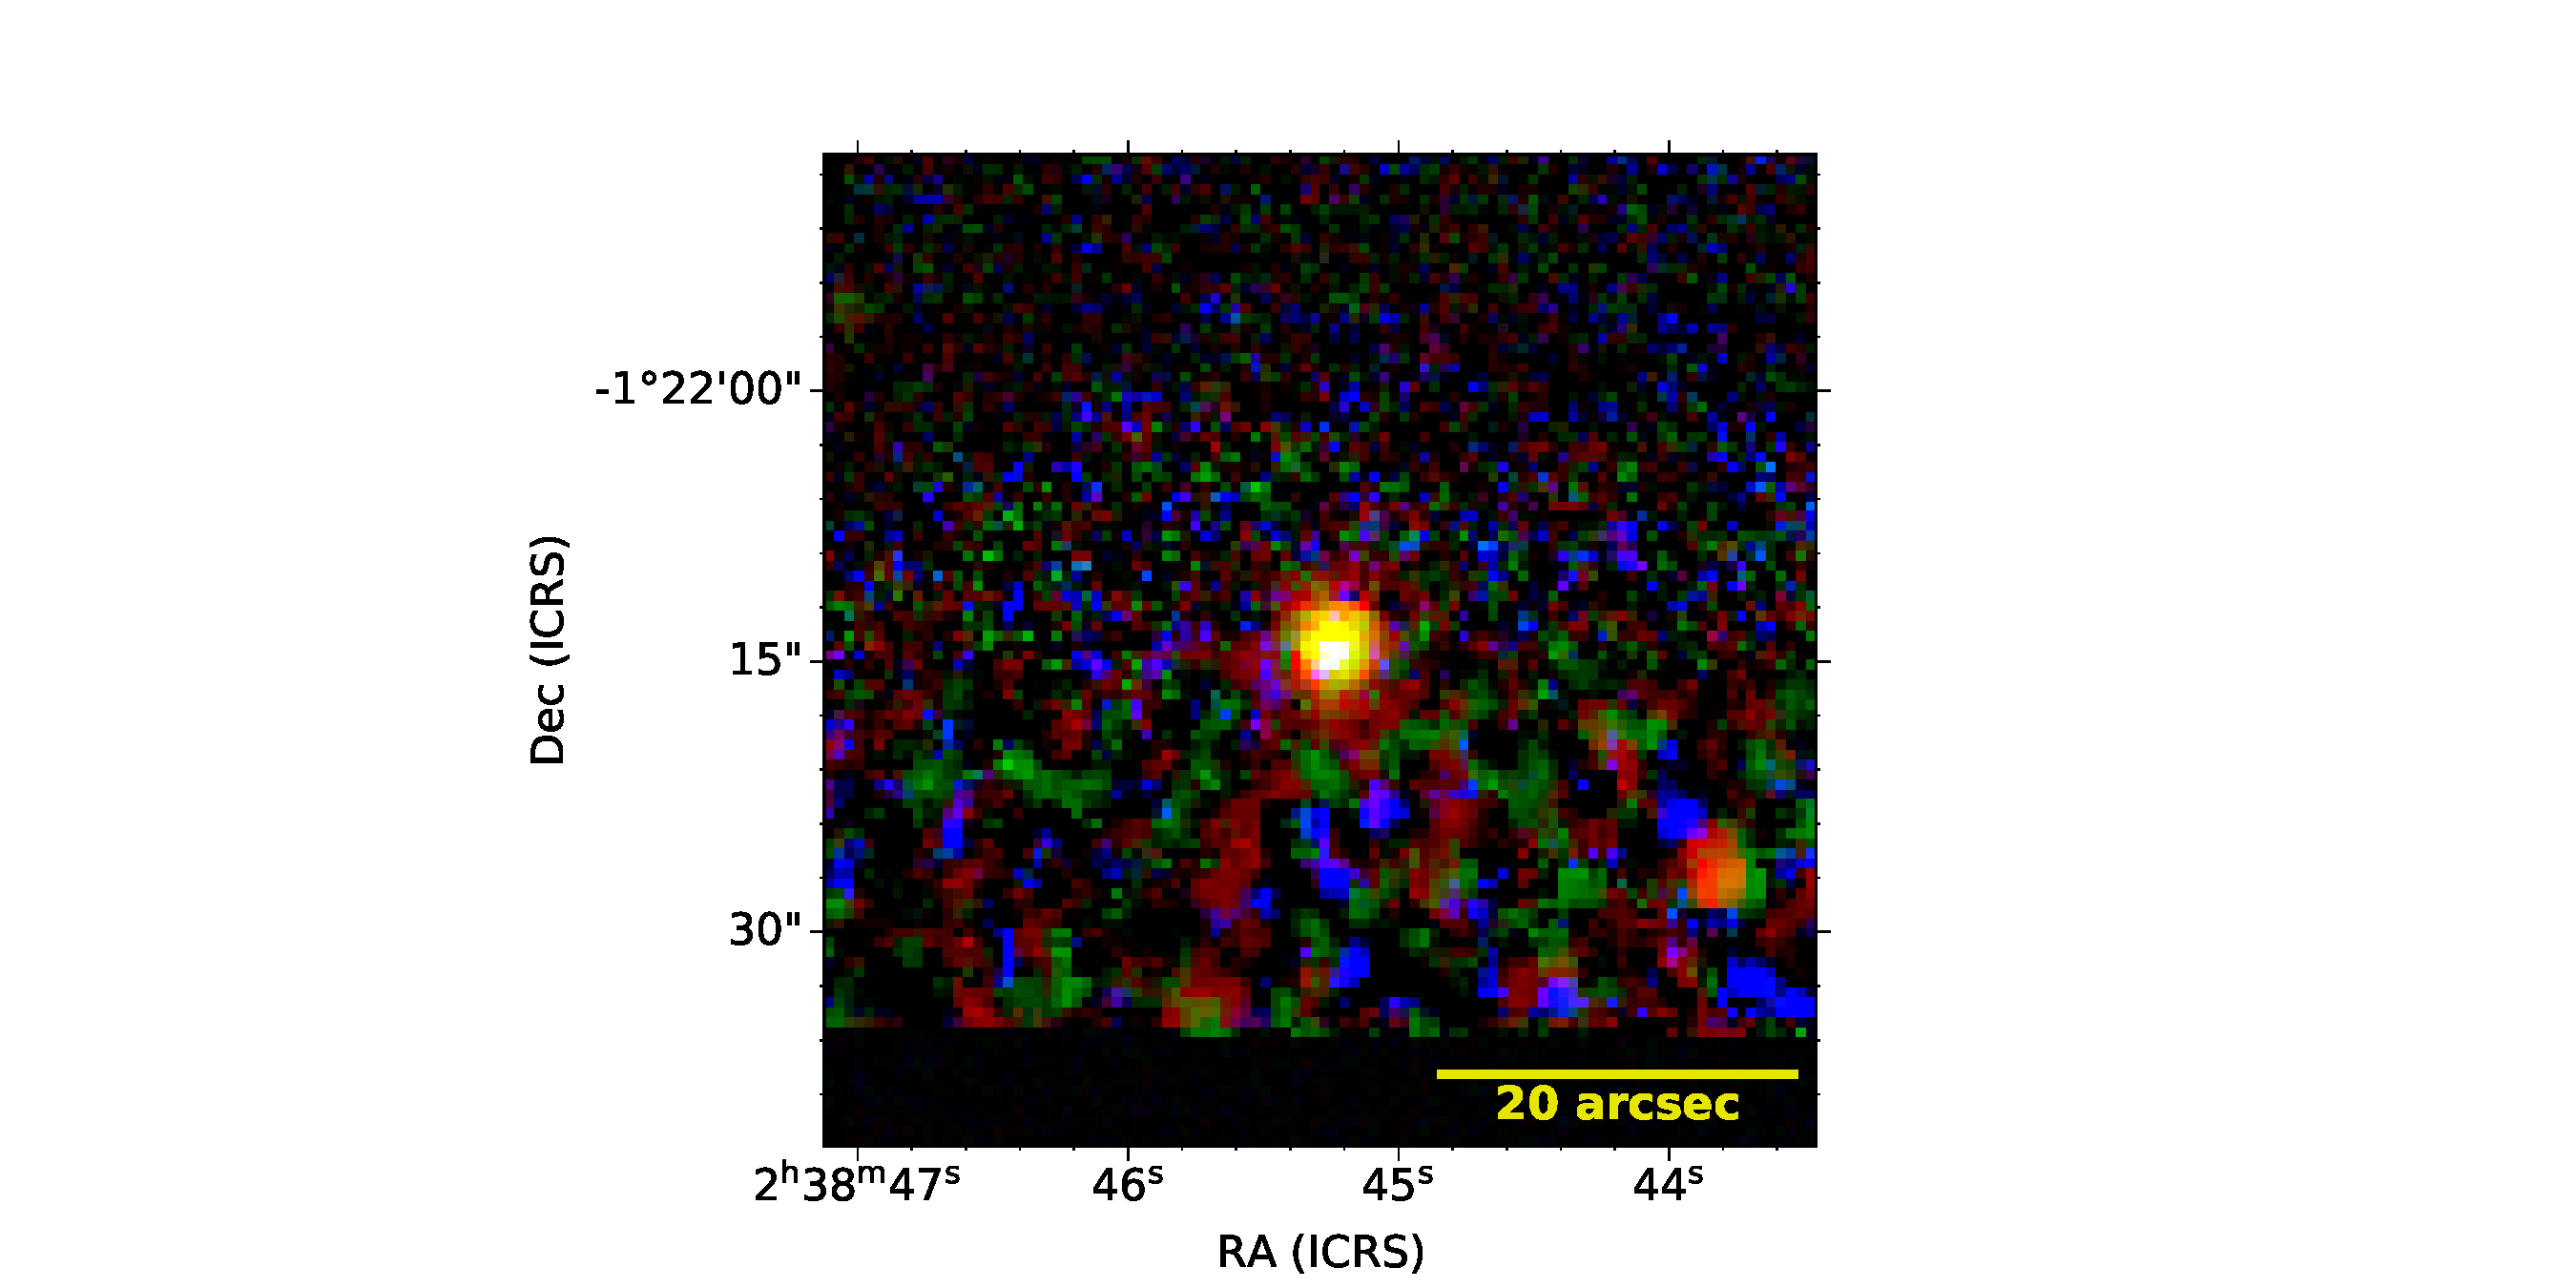
\includegraphics[width=0.3\linewidth, trim=10 0 65 20, clip]{Figs/STRIPE82-0057-001810_39-1_100_r.pdf} \\
    (c) & (d) \\
    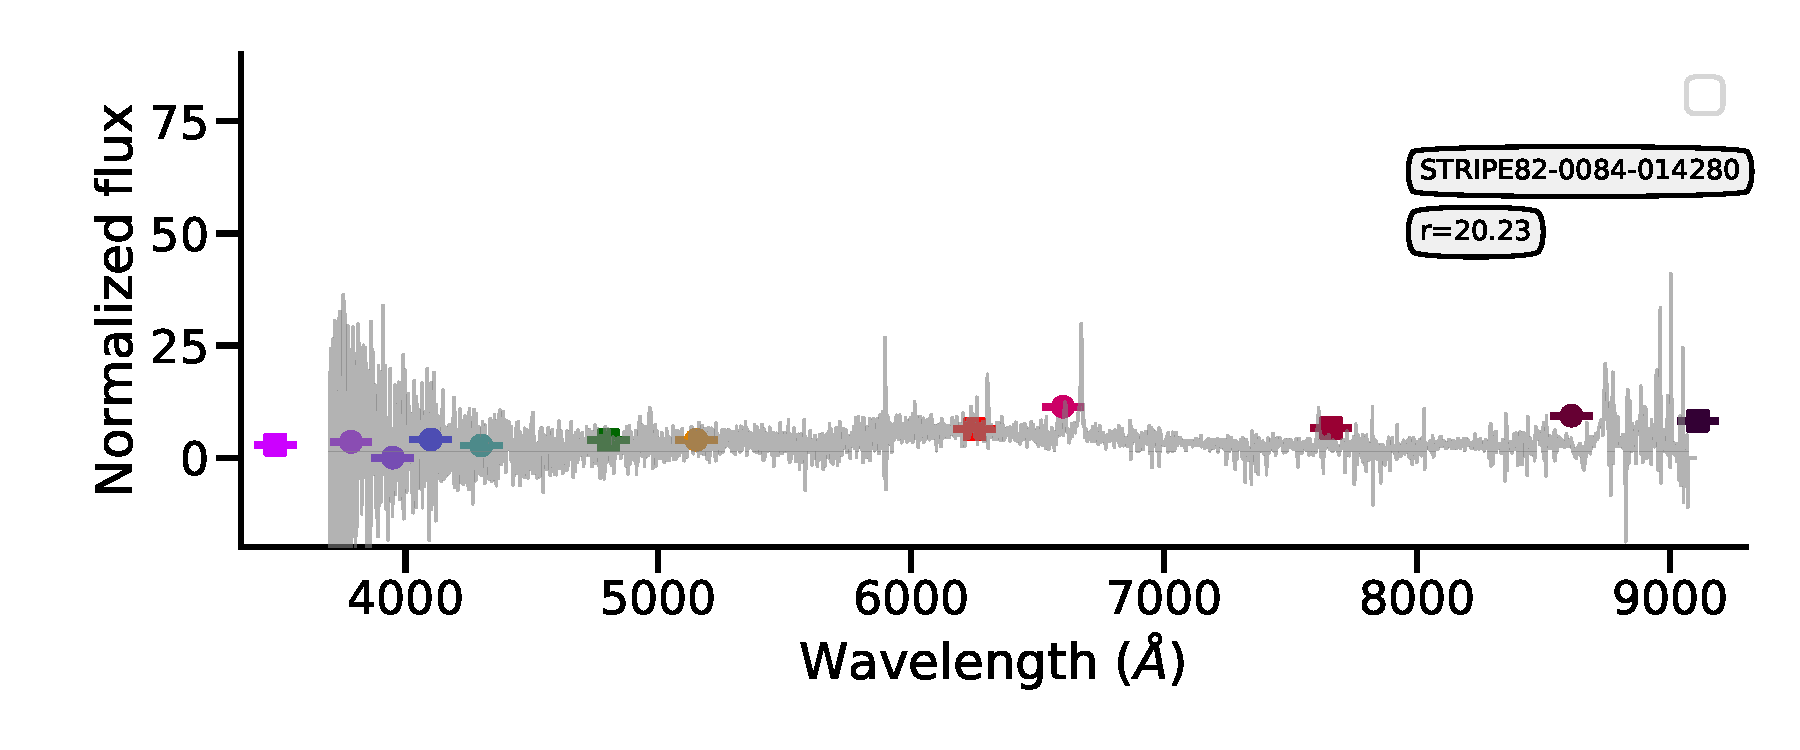
\includegraphics[trim=10 0 10 20, clip]{Figs/spec-57336-EG034838N001340M01_sp09-025-STRIPE82-0084-014280.pdf} & 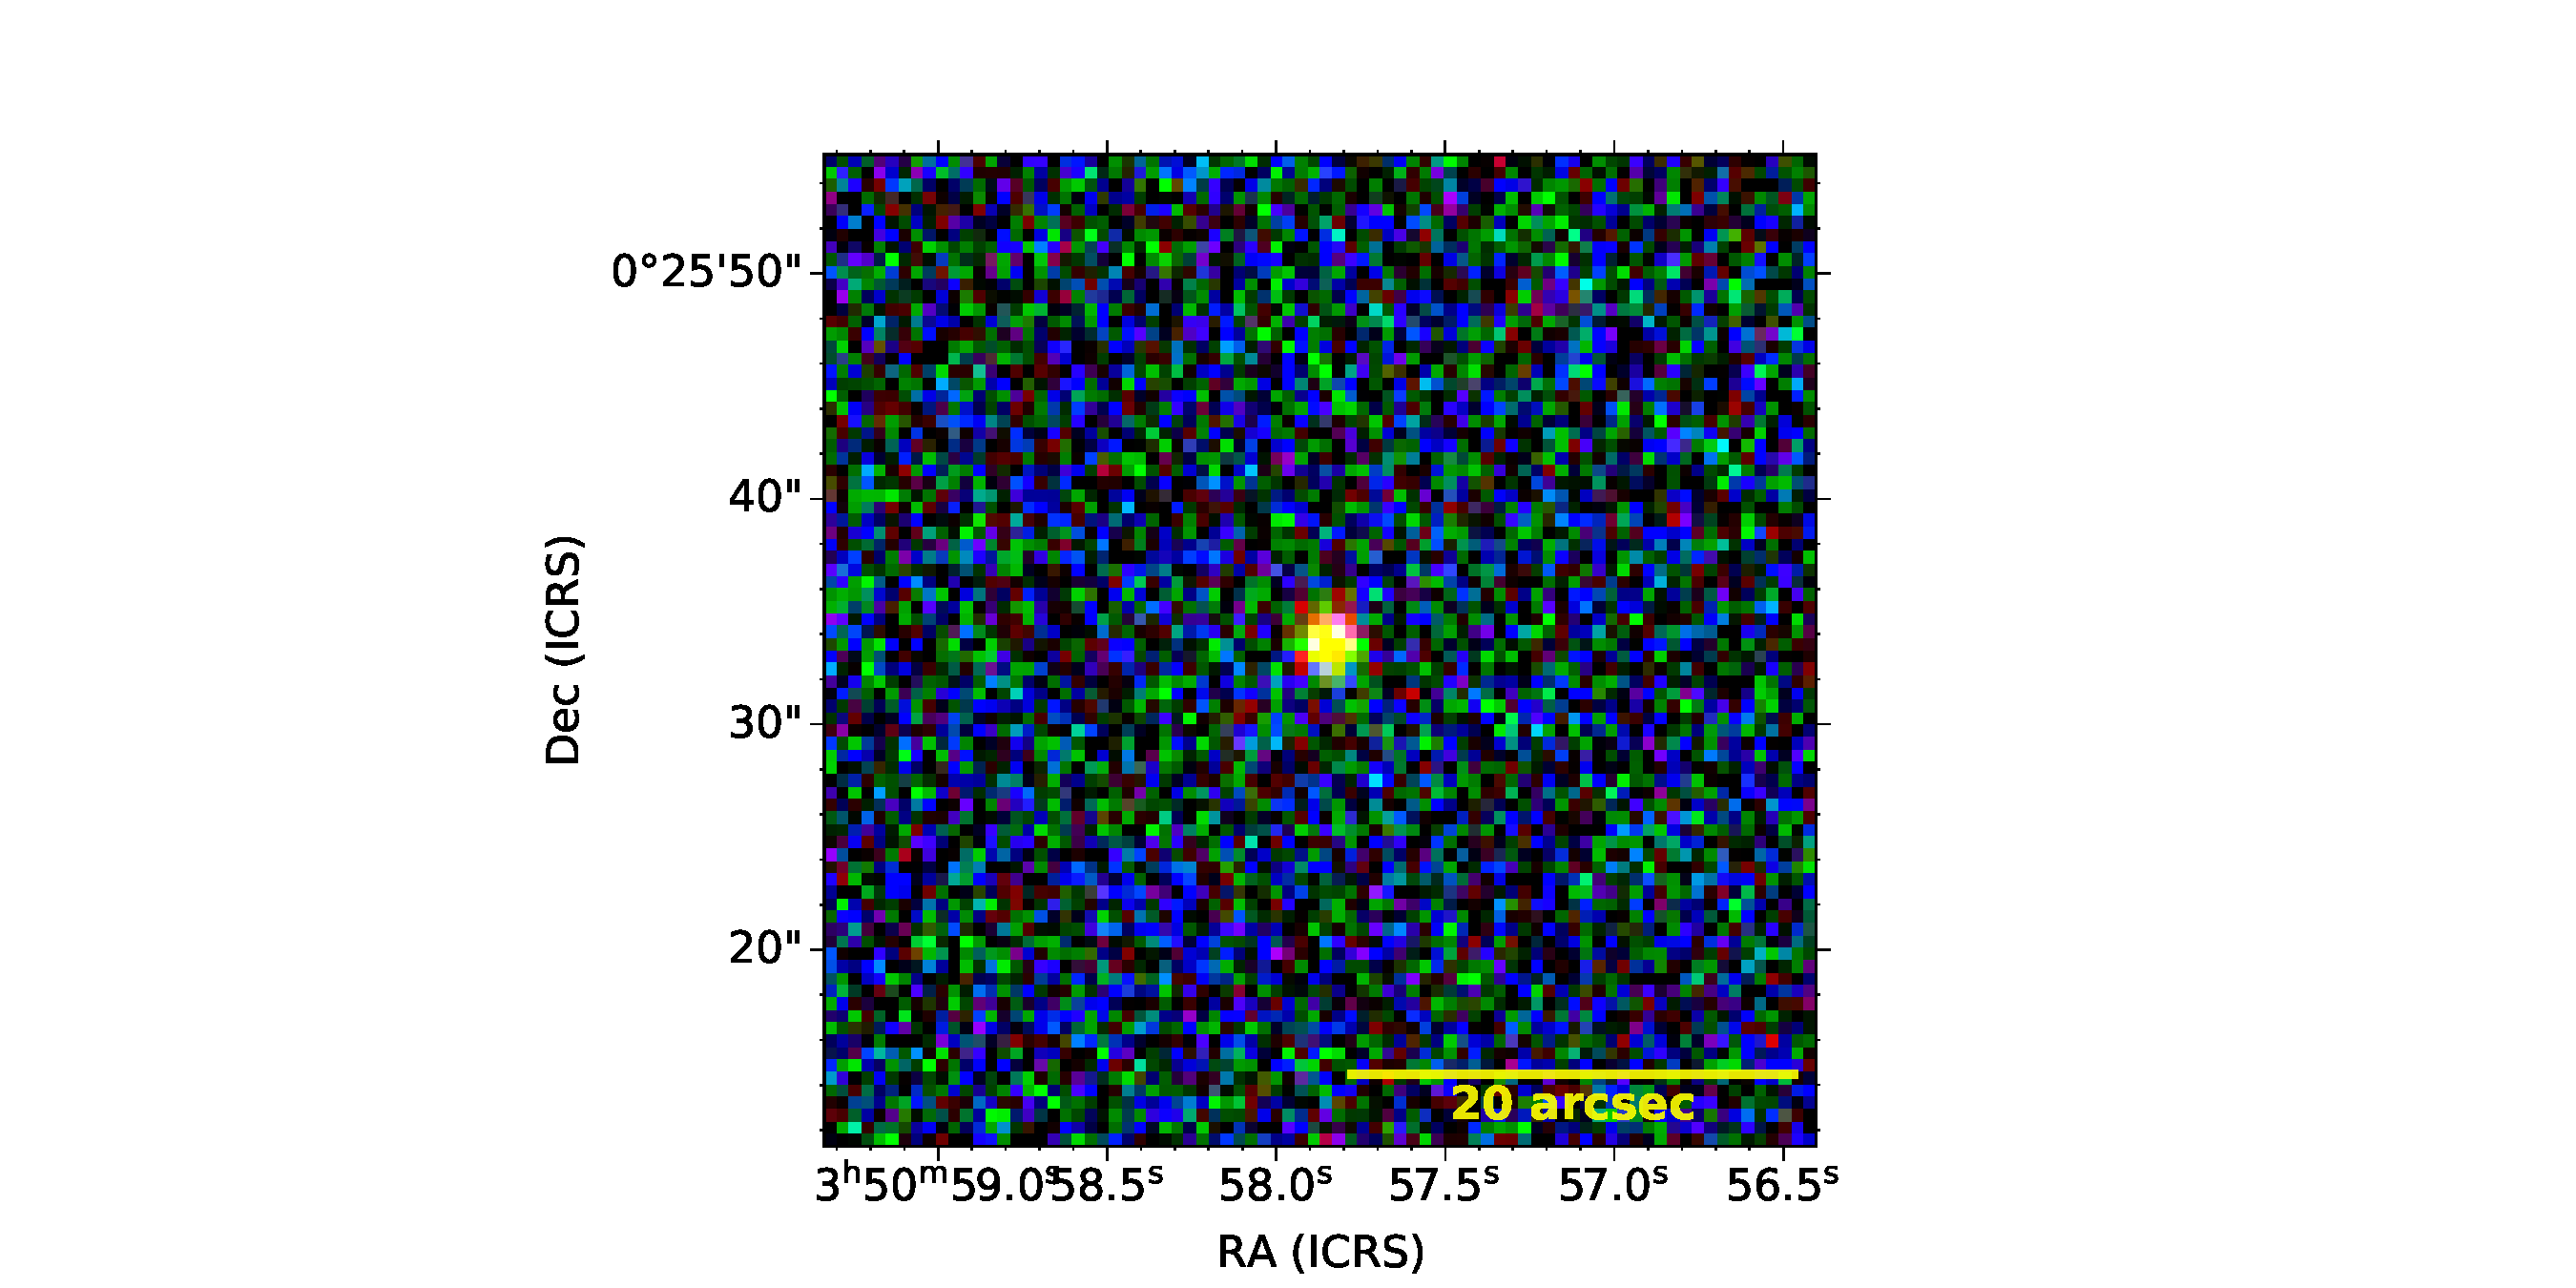
\includegraphics[width=0.3\linewidth, trim=10 0 65 20, clip]{Figs/STRIPE82-0084-014280_57-0_80_r.pdf} \\
  \end{tabular}
  \caption{Spectra of the Lamost }
  \label{fig:color-diagram}
\end{figure*}

\begin{figure*}
  \setlength\tabcolsep{0pt}
  \setkeys{Gin}{width=0.5\linewidth}
  \begin{tabular}{ll}
    (a) & (b) \\
    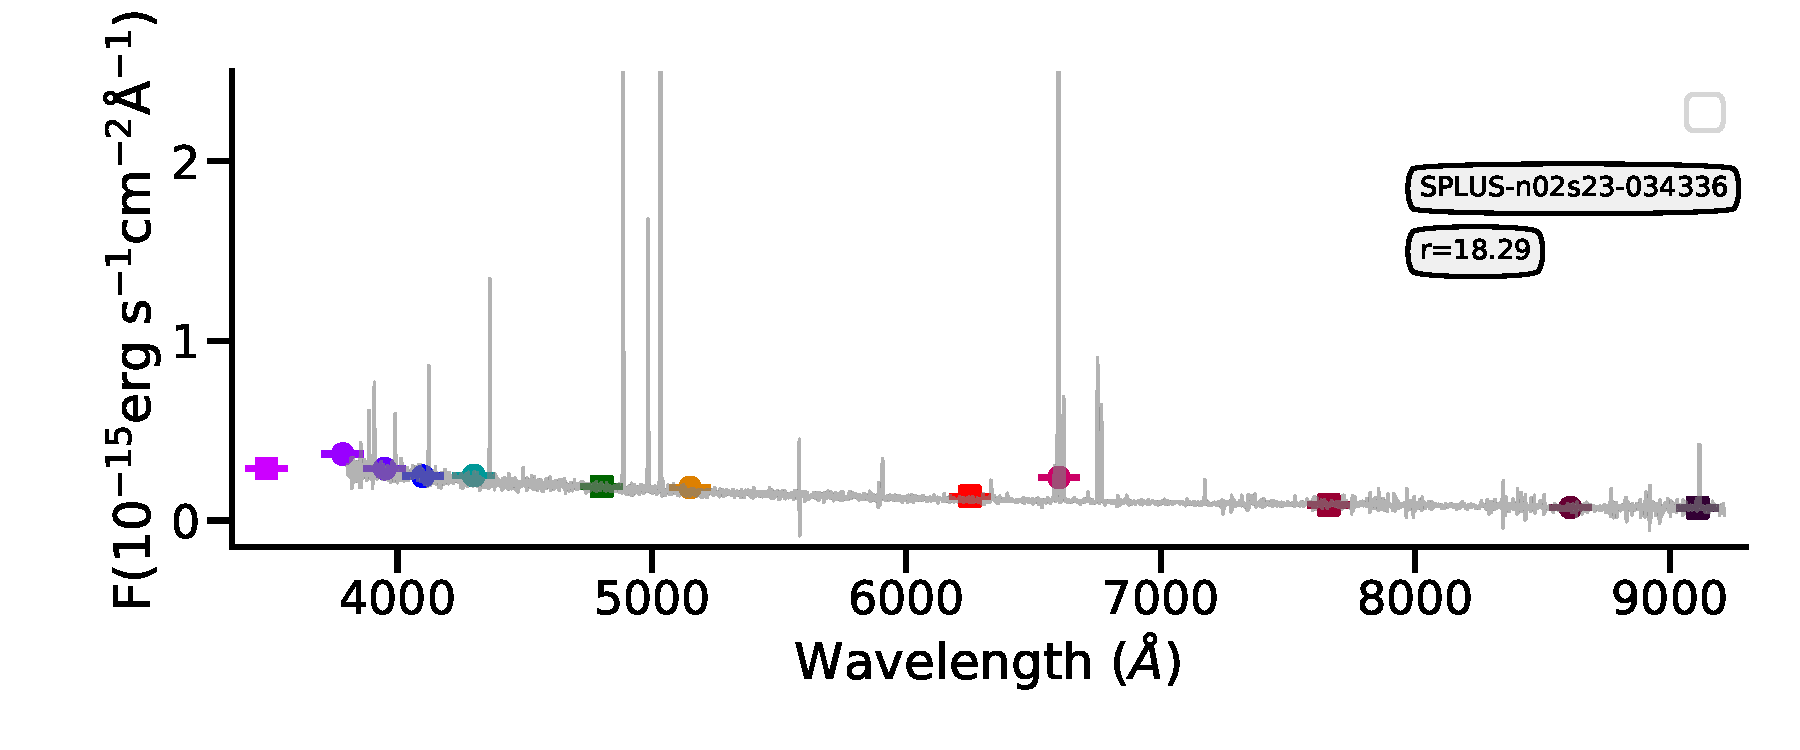
\includegraphics[trim=10 0 10 20, clip]{Figs/spec-0331-52368-0449-SPLUS-n02s23-034336.pdf} & 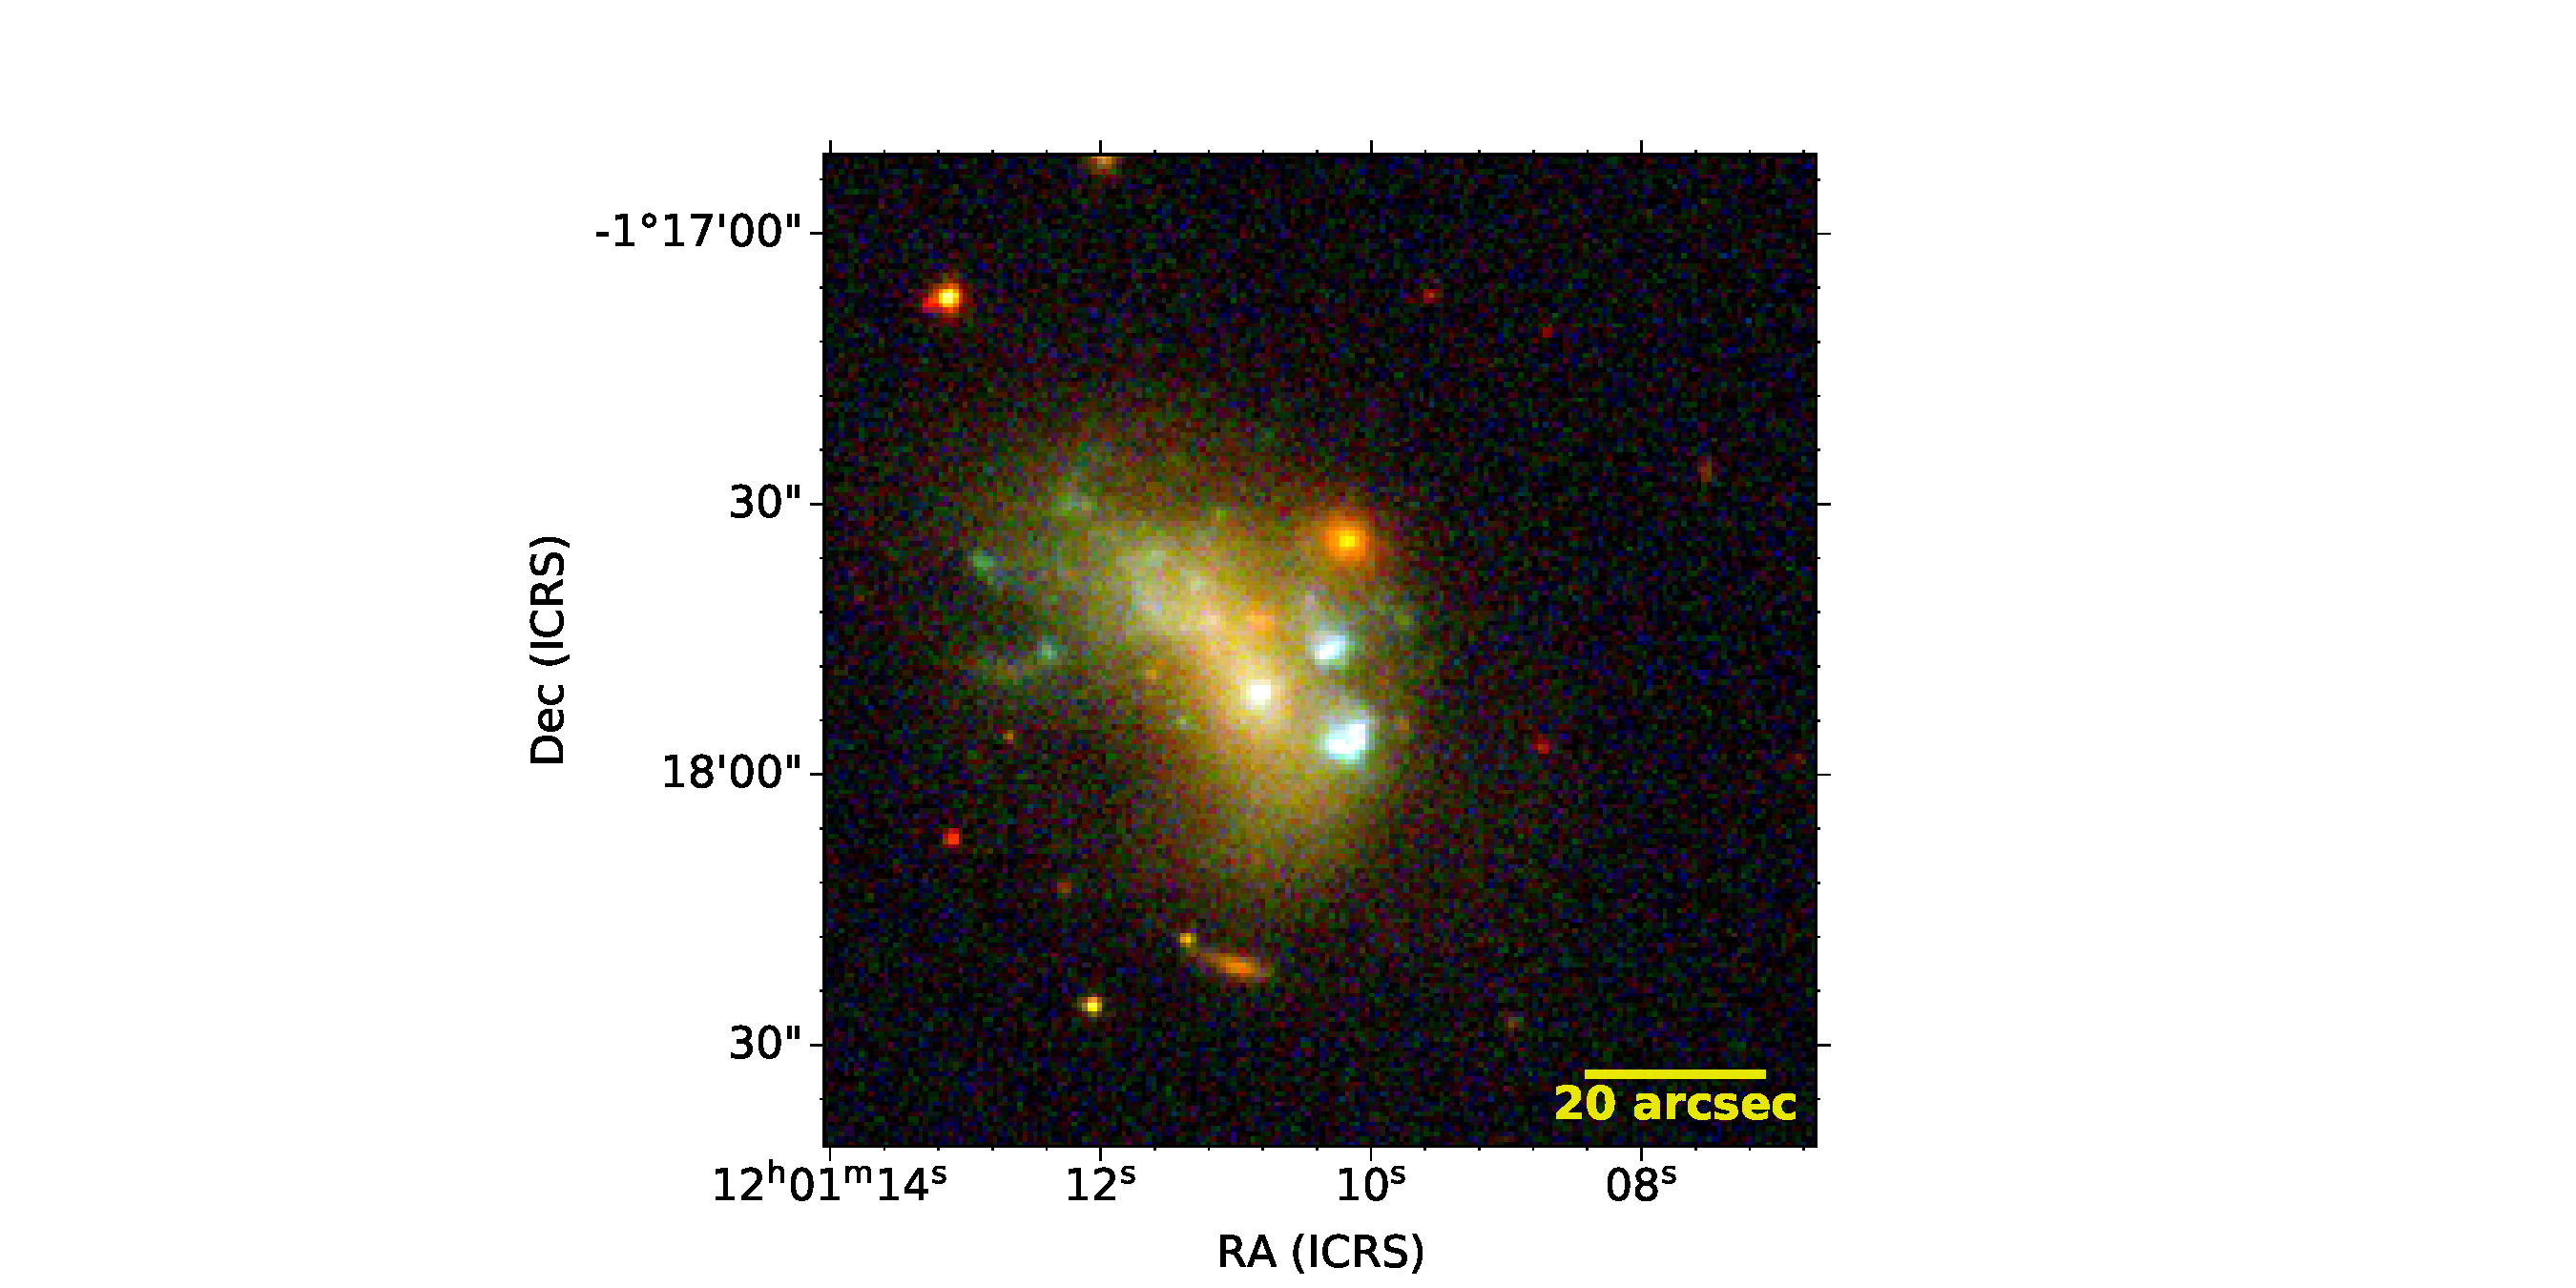
\includegraphics[width=0.3\linewidth, trim=10 0 65 20, clip]{Figs/SPLUS-n02s23-034336_180-1_200_r.pdf} \\
     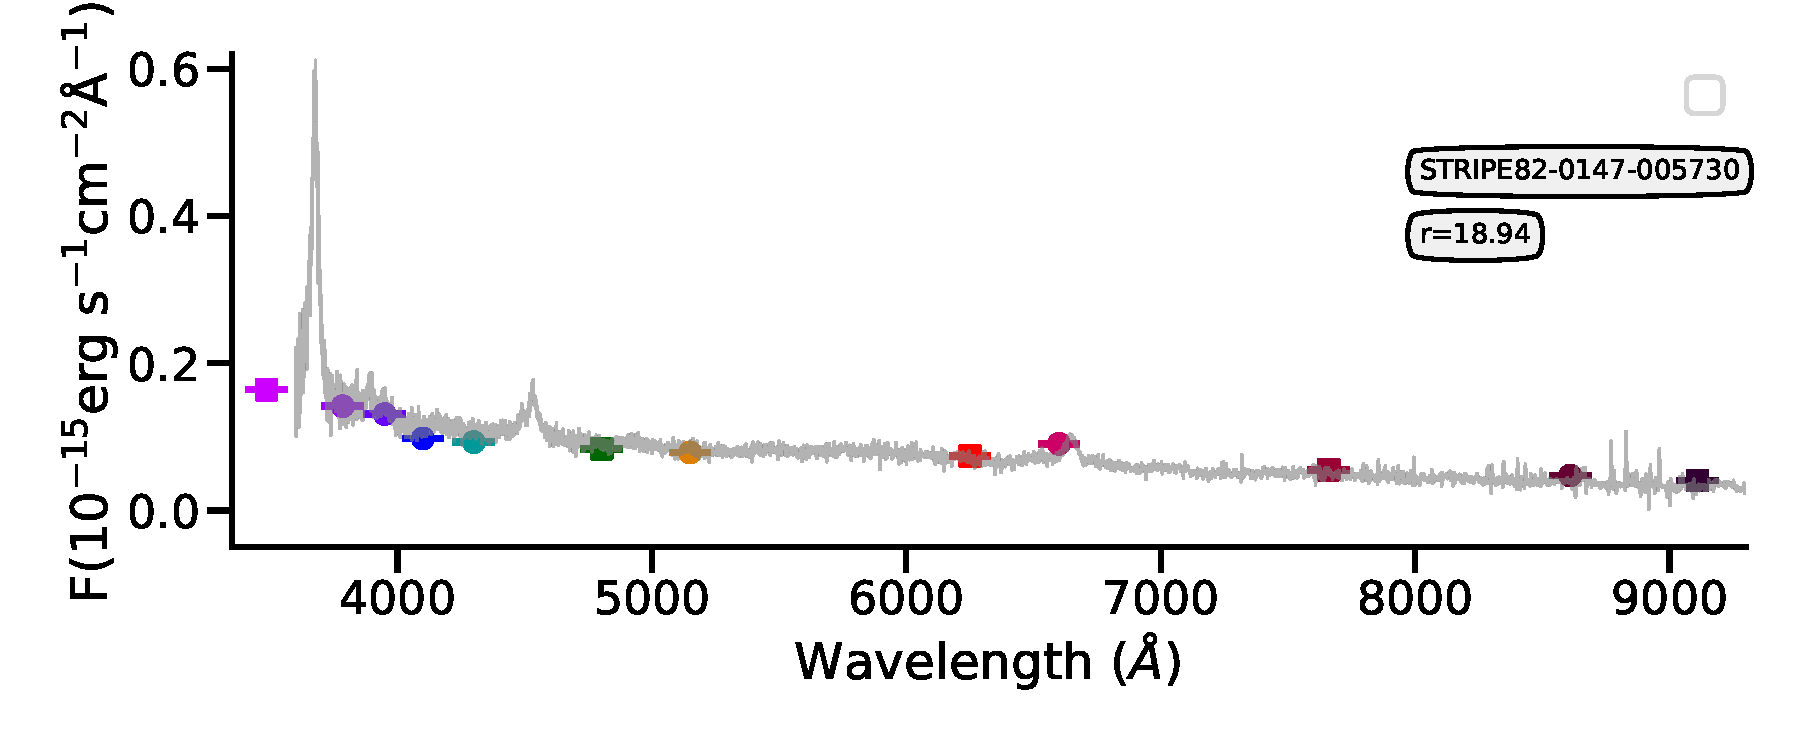
\includegraphics[trim=10 0 10 20, clip]{Figs/spec-9152-58041-0463-STRIPE82-0147-005730.pdf} & 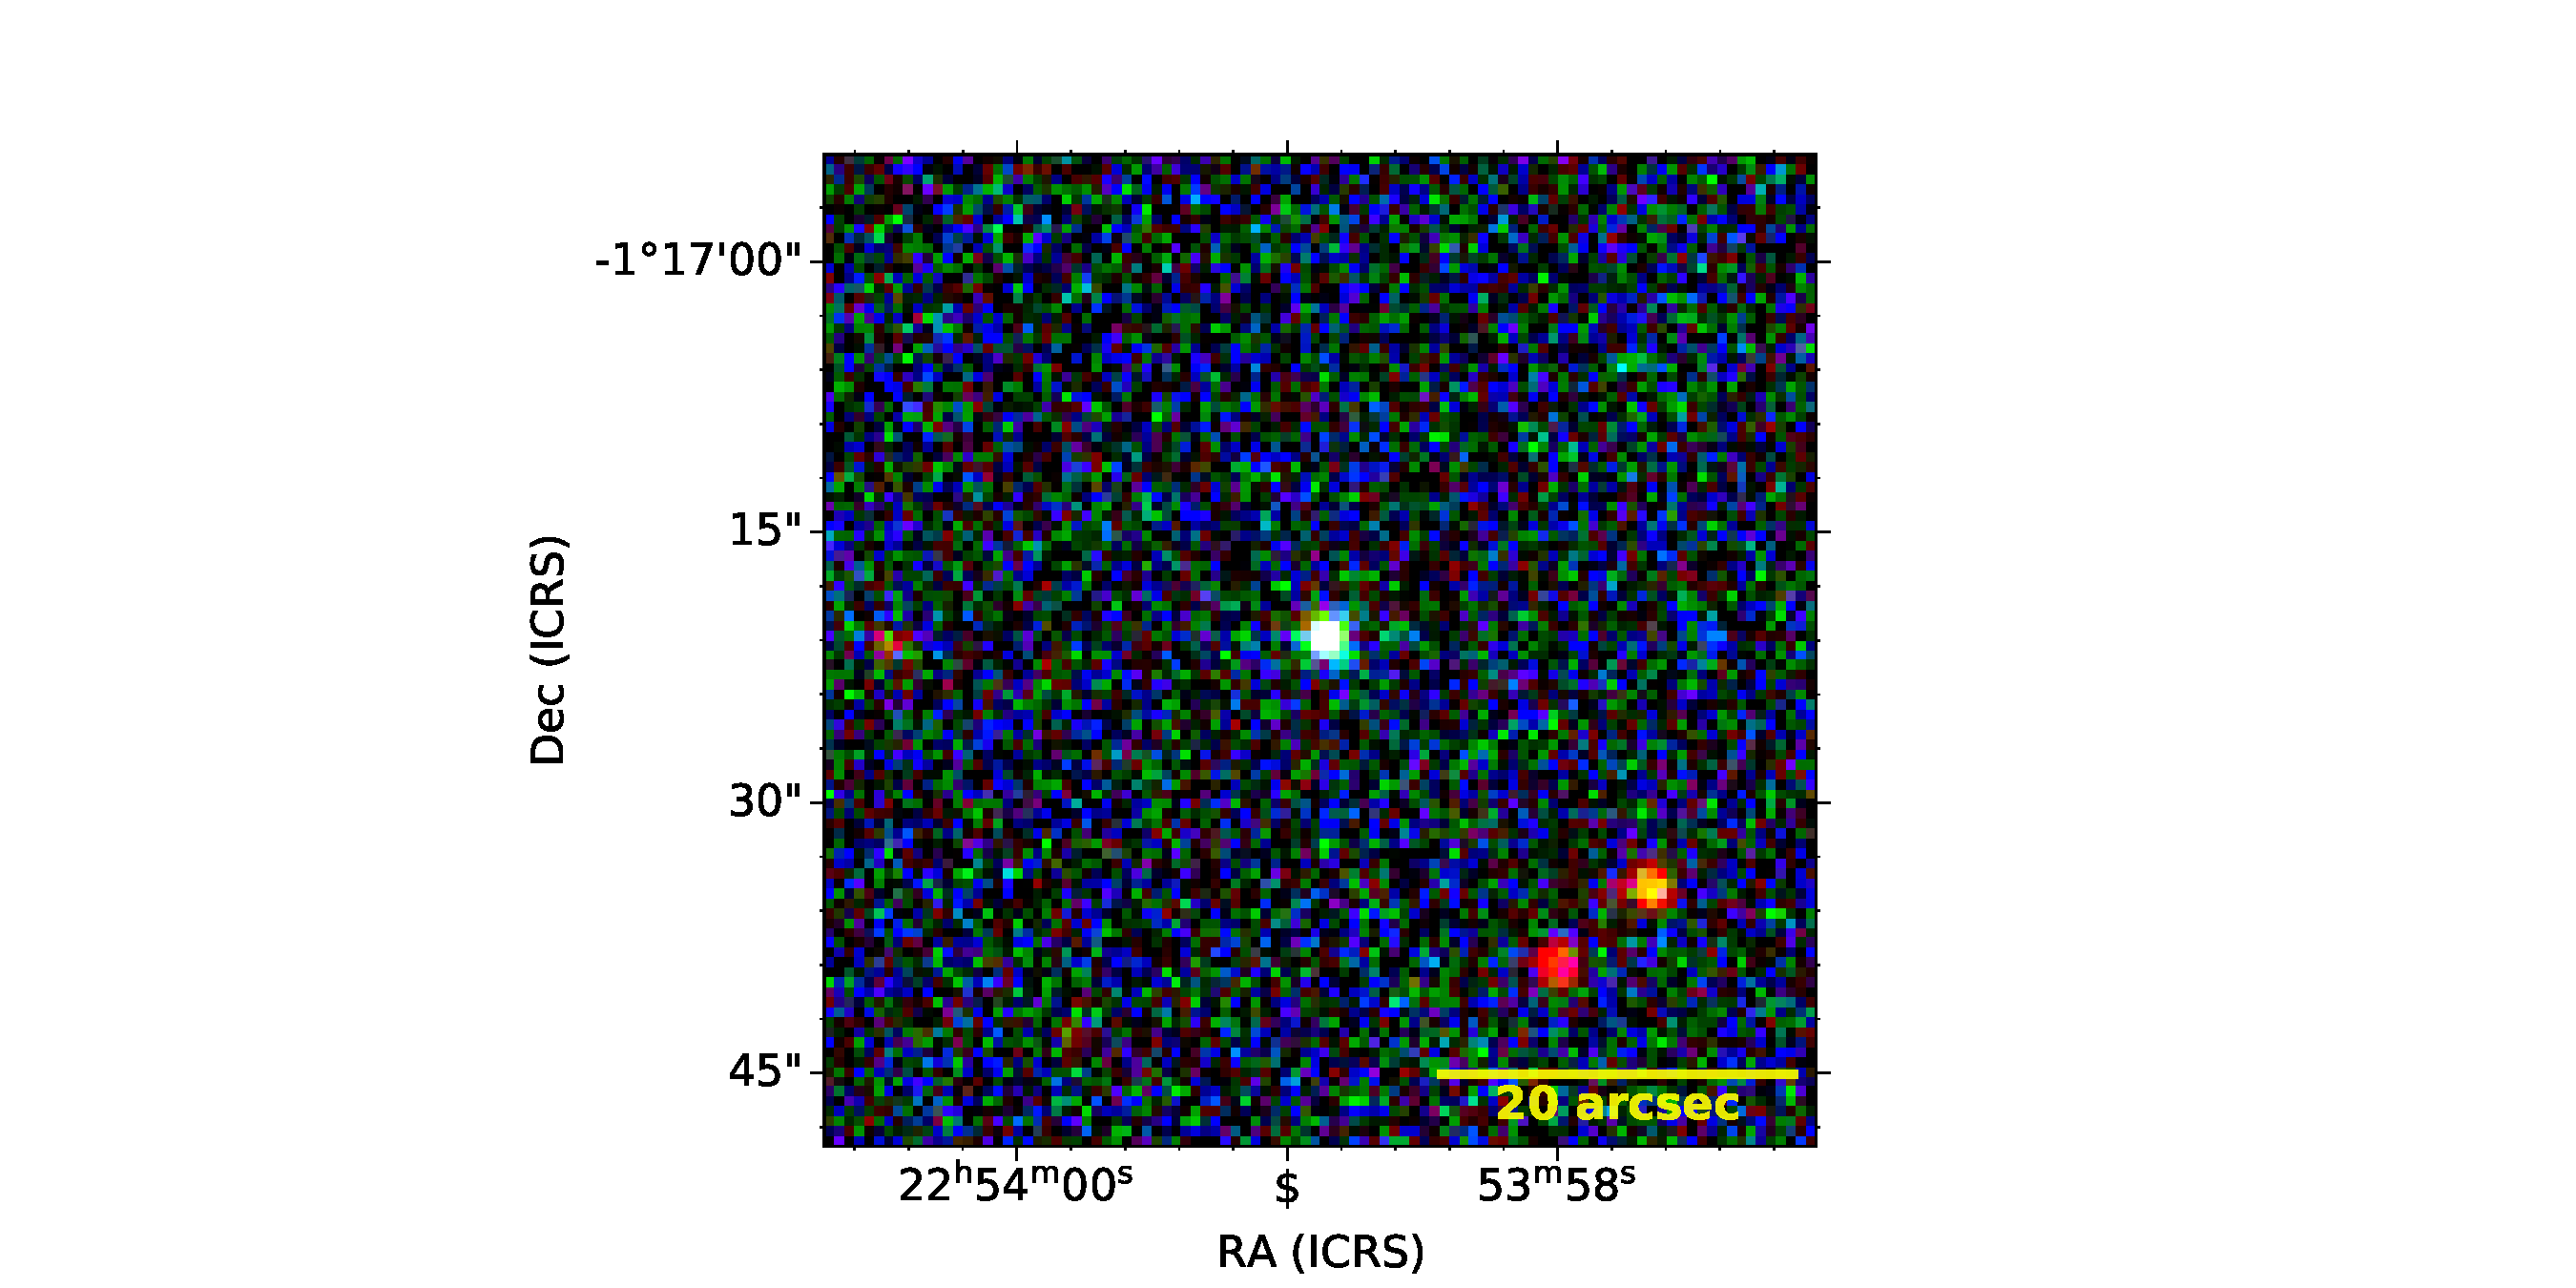
\includegraphics[width=0.3\linewidth, trim=10 0 65 20, clip]{Figs/STRIPE82-0147-005730_343-1_100_r.pdf} \\
    (c) & (d) \\
    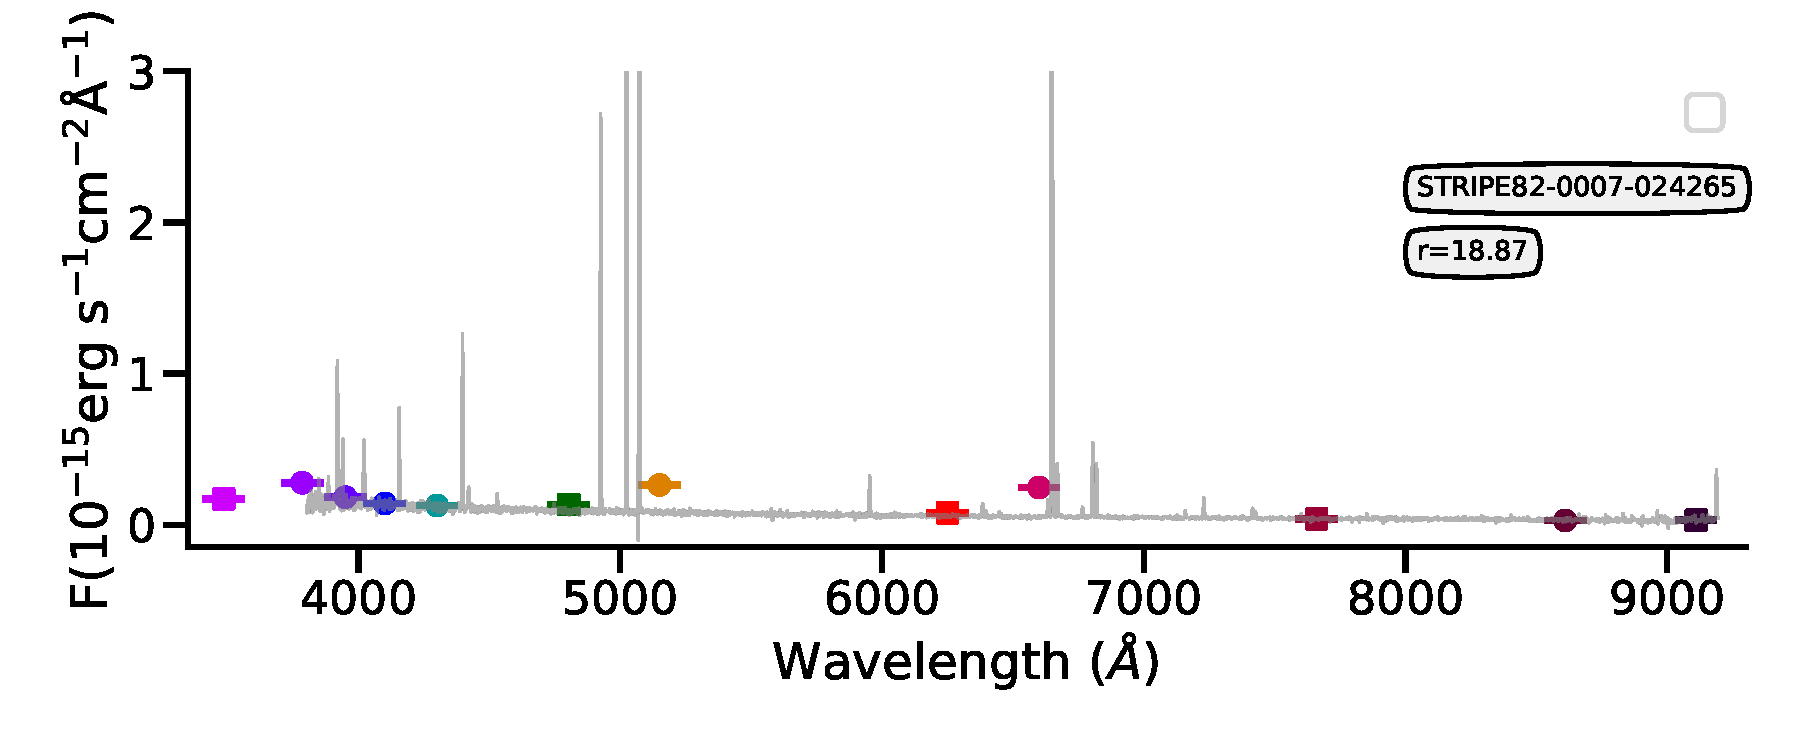
\includegraphics[trim=10 0 10 20, clip]{Figs/spec-1089-52913-0196-STRIPE82-0007-024265.pdf} & 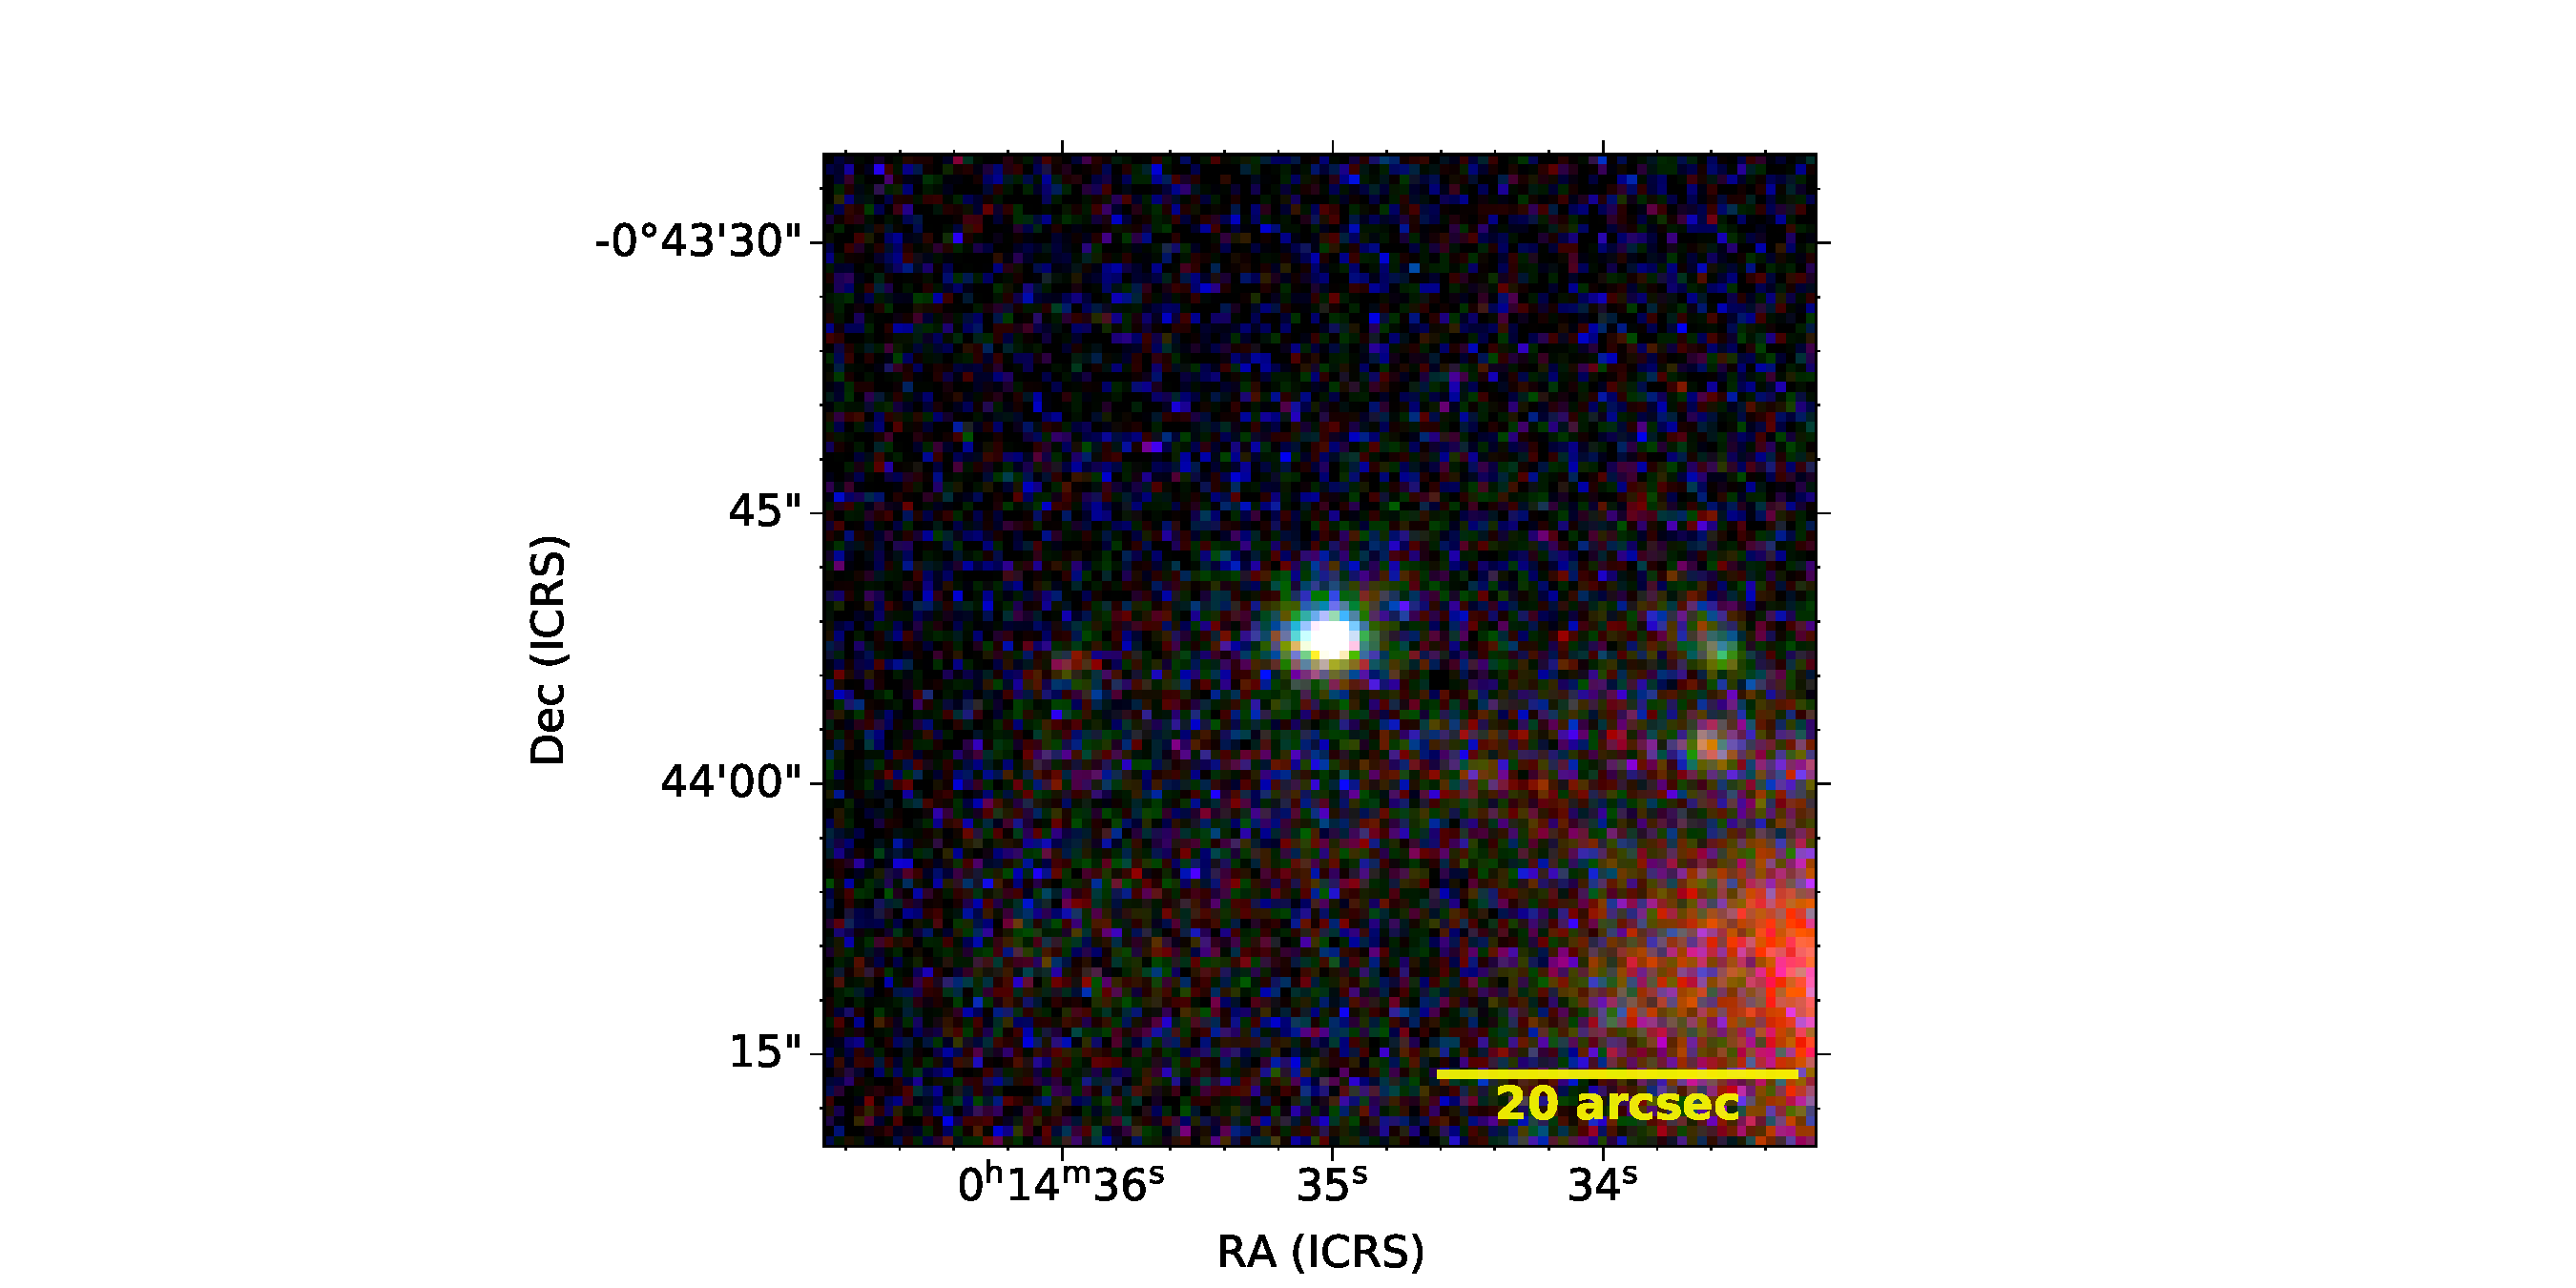
\includegraphics[width=0.3\linewidth, trim=10 0 65 20, clip]{Figs/STRIPE82-0007-024265_3-0_100_r.pdf} \\
  \end{tabular}
  \caption{Spectra of the SDSS}
  \label{fig:color-diagram}
\end{figure*}

\section{Conclusions}

We have found a important sample of emission line objects.

\section*{Acknowledgements}


%%%%%%%%%%%%%%%%%%%%%%%%%%%%%%%%%%%%%%%%%%%%%%%%%%
\section*{Data Availability}



%%%%%%%%%%%%%%%%%%%% REFERENCES %%%%%%%%%%%%%%%%%%

% The best way to enter references is to use BibTeX:

\bibliographystyle{mnras}
\bibliography{ref} % if your bibtex file is called example.bib


% Alternatively you could enter them by hand, like this:
% This method is tedious and prone to error if you have lots of references
%\begin{thebibliography}{99}
%\bibitem[\protect\citeauthoryear{Author}{2012}]{Author2012}
%Author A.~N., 2013, Journal of Improbable Astronomy, 1, 1
%\bibitem[\protect\citeauthoryear{Others}{2013}]{Others2013}
%Others S., 2012, Journal of Interesting Stuff, 17, 198
%\end{thebibliography}

%%%%%%%%%%%%%%%%%%%%%%%%%%%%%%%%%%%%%%%%%%%%%%%%%%

%%%%%%%%%%%%%%%%% APPENDICES %%%%%%%%%%%%%%%%%%%%%

\appendix

\section{Some extra material}


%%%%%%%%%%%%%%%%%%%%%%%%%%%%%%%%%%%%%%%%%%%%%%%%%%


% Don't change these lines
\bsp	% typesetting comment
\label{lastpage}
\end{document}

% End of mnras_template.tex
